% !TEX root =  ../../../thesis.tex

\section{Experimental Results}\label{sec:aam:experiments}
Herein, we present extended experiments for both face alignment (LK,
Sec.~\ref{subsec:aam:faceAlignment}) and face fitting (holistic AAMs,
Secs.~\ref{subsec:aam:AAMs} and \ref{subsec:aam:comparison}) using the IC
framework. We employ all the dense features described in
Sec.~\ref{sec:aam:features} with the parameters of
Tab.~\ref{tab:featuresParameters}.

Note that commonly LK and AAMs fitting is performed using an
image pyramid with progressively increasing the number of shape and appearance
parameters as the image resolution
increases~\cite{baker2004lucas,matthews2004active,papandreou2008adaptive,tzimiropoulos2011robust}.
However, in the following experiments of this chapter, the image pyramid is not
employed in order to facilitate and simplify the comparisons. Using multiple
fitting scales would make it difficult to derive any conclusions about the
various features and approaches, such as the representation power, number of
appearance and shape eigenvectors, convergence rate, etc. Nevertheless, a
multi-level pyramid fitting framework is employed in the rest of this thesis,
as also explained in individual Chapters~\ref{ch:aps}, \ref{ch:automatic_training}
and \ref{ch:acr}.

% Yale B examples
\begin{figure}[!h]
\centering
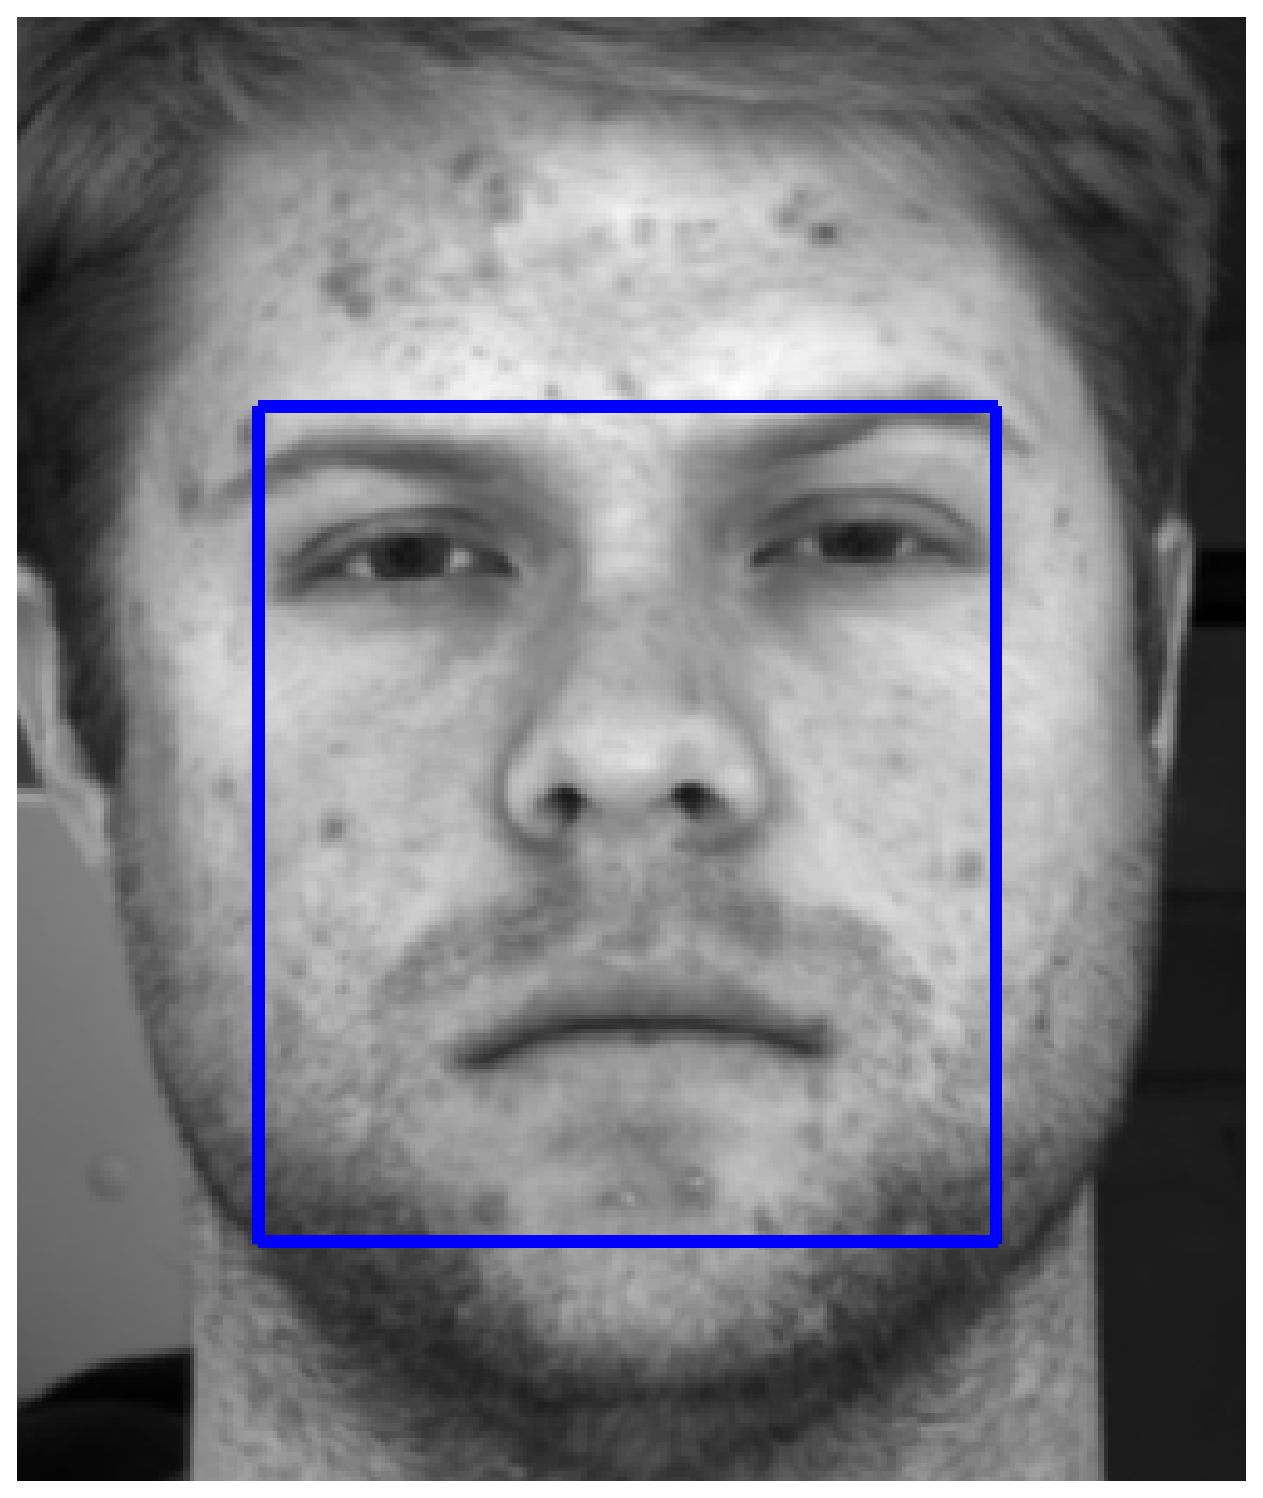
\includegraphics[width=0.18\linewidth]{figures/feature_based_aam/3_YaleB/1a}\hspace{0.4cm}
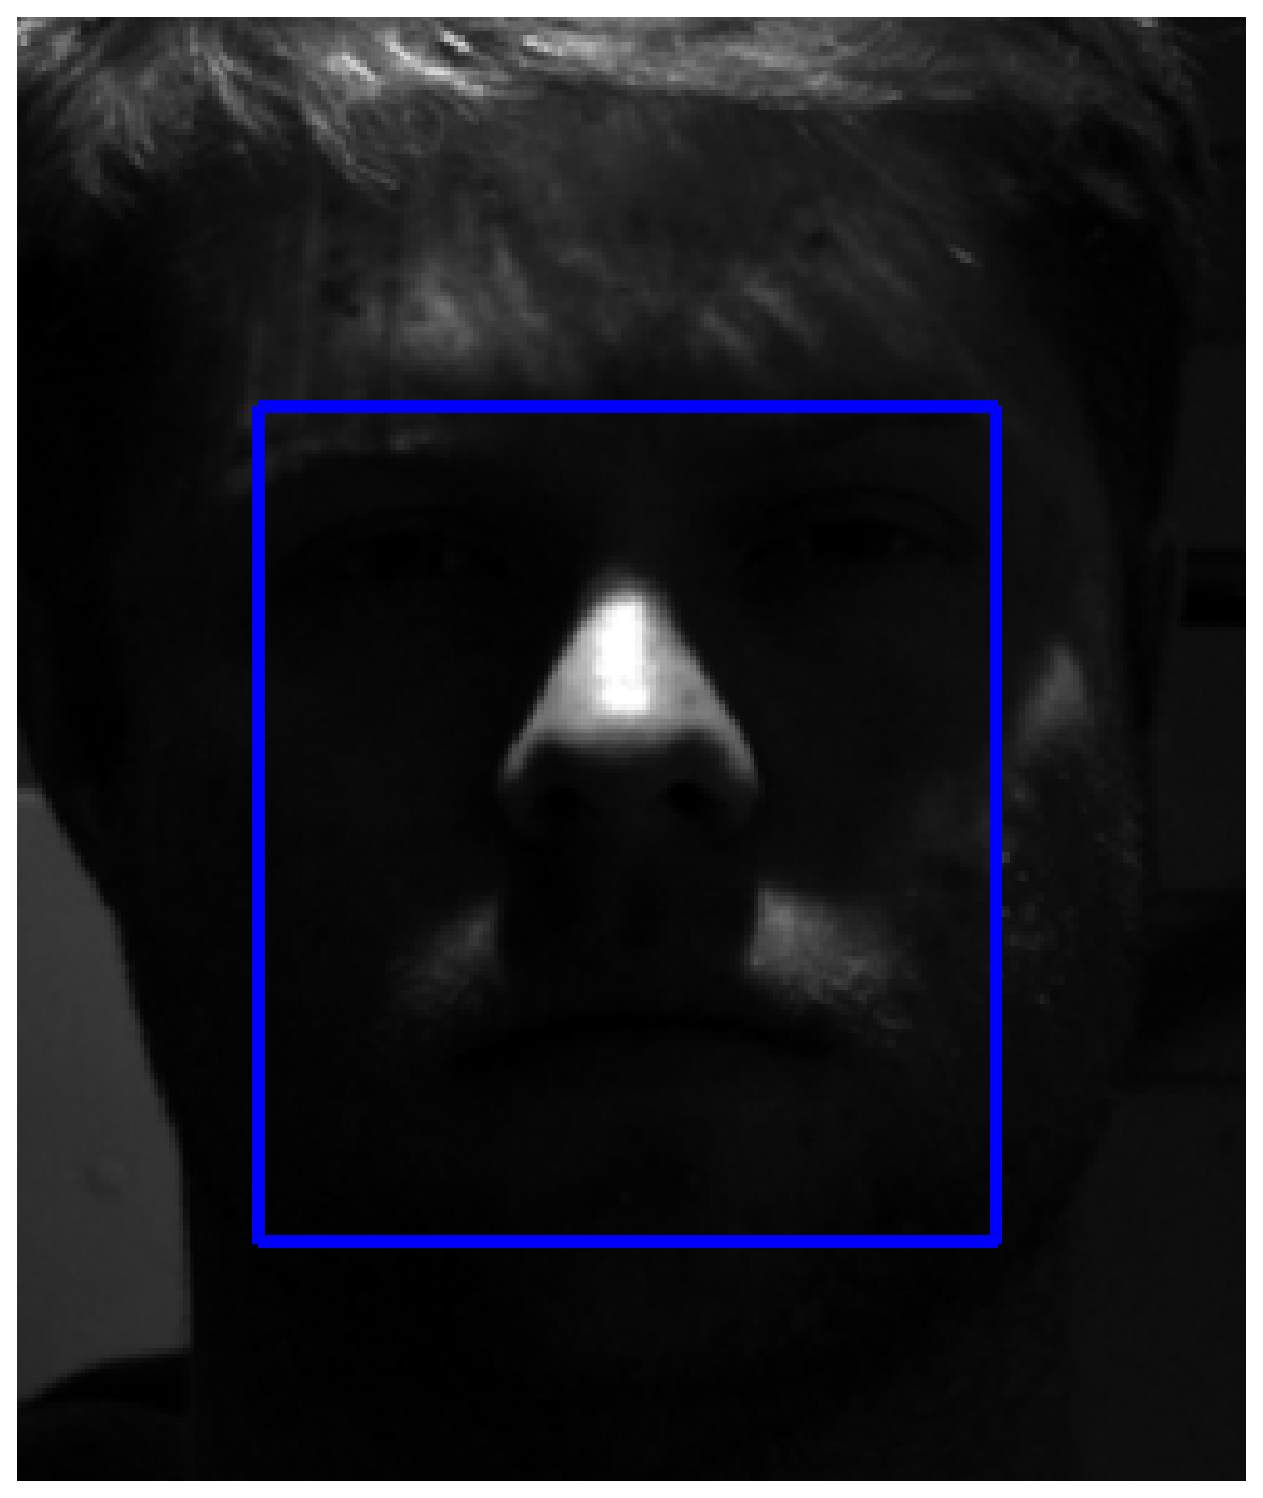
\includegraphics[width=0.18\linewidth]{figures/feature_based_aam/3_YaleB/1b}
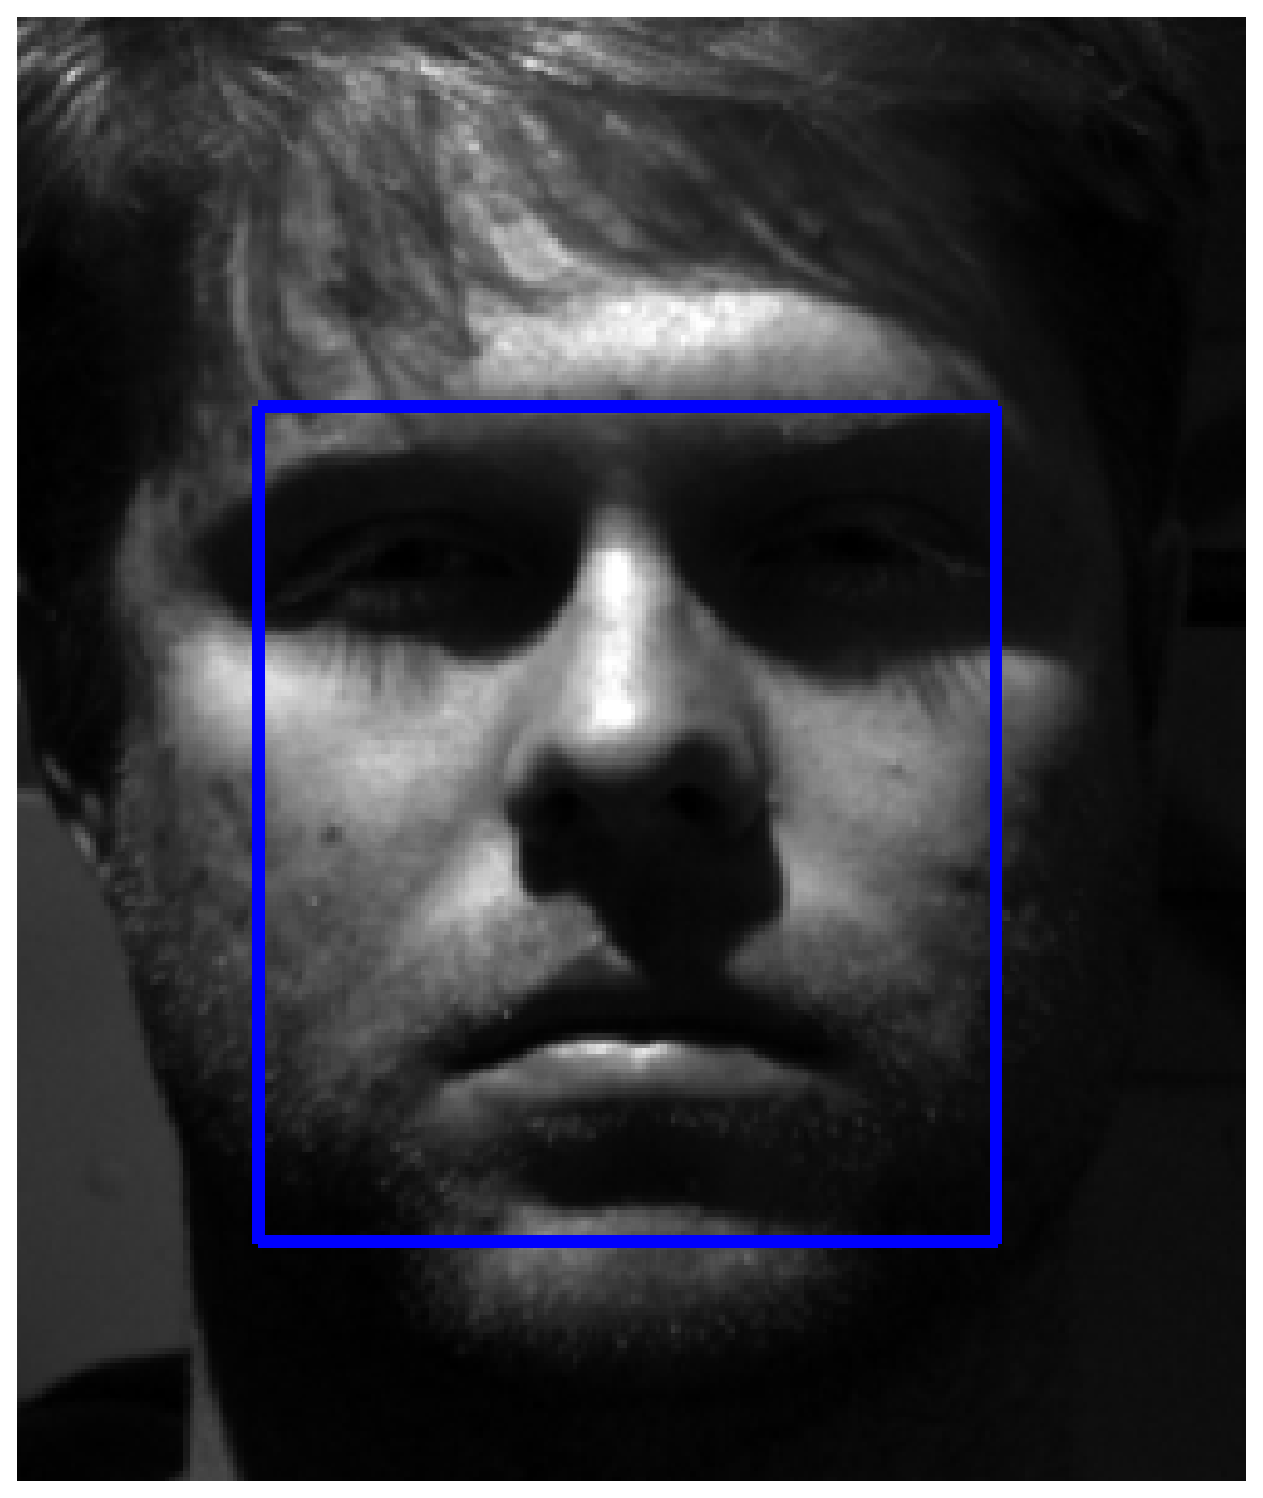
\includegraphics[width=0.18\linewidth]{figures/feature_based_aam/3_YaleB/1c}
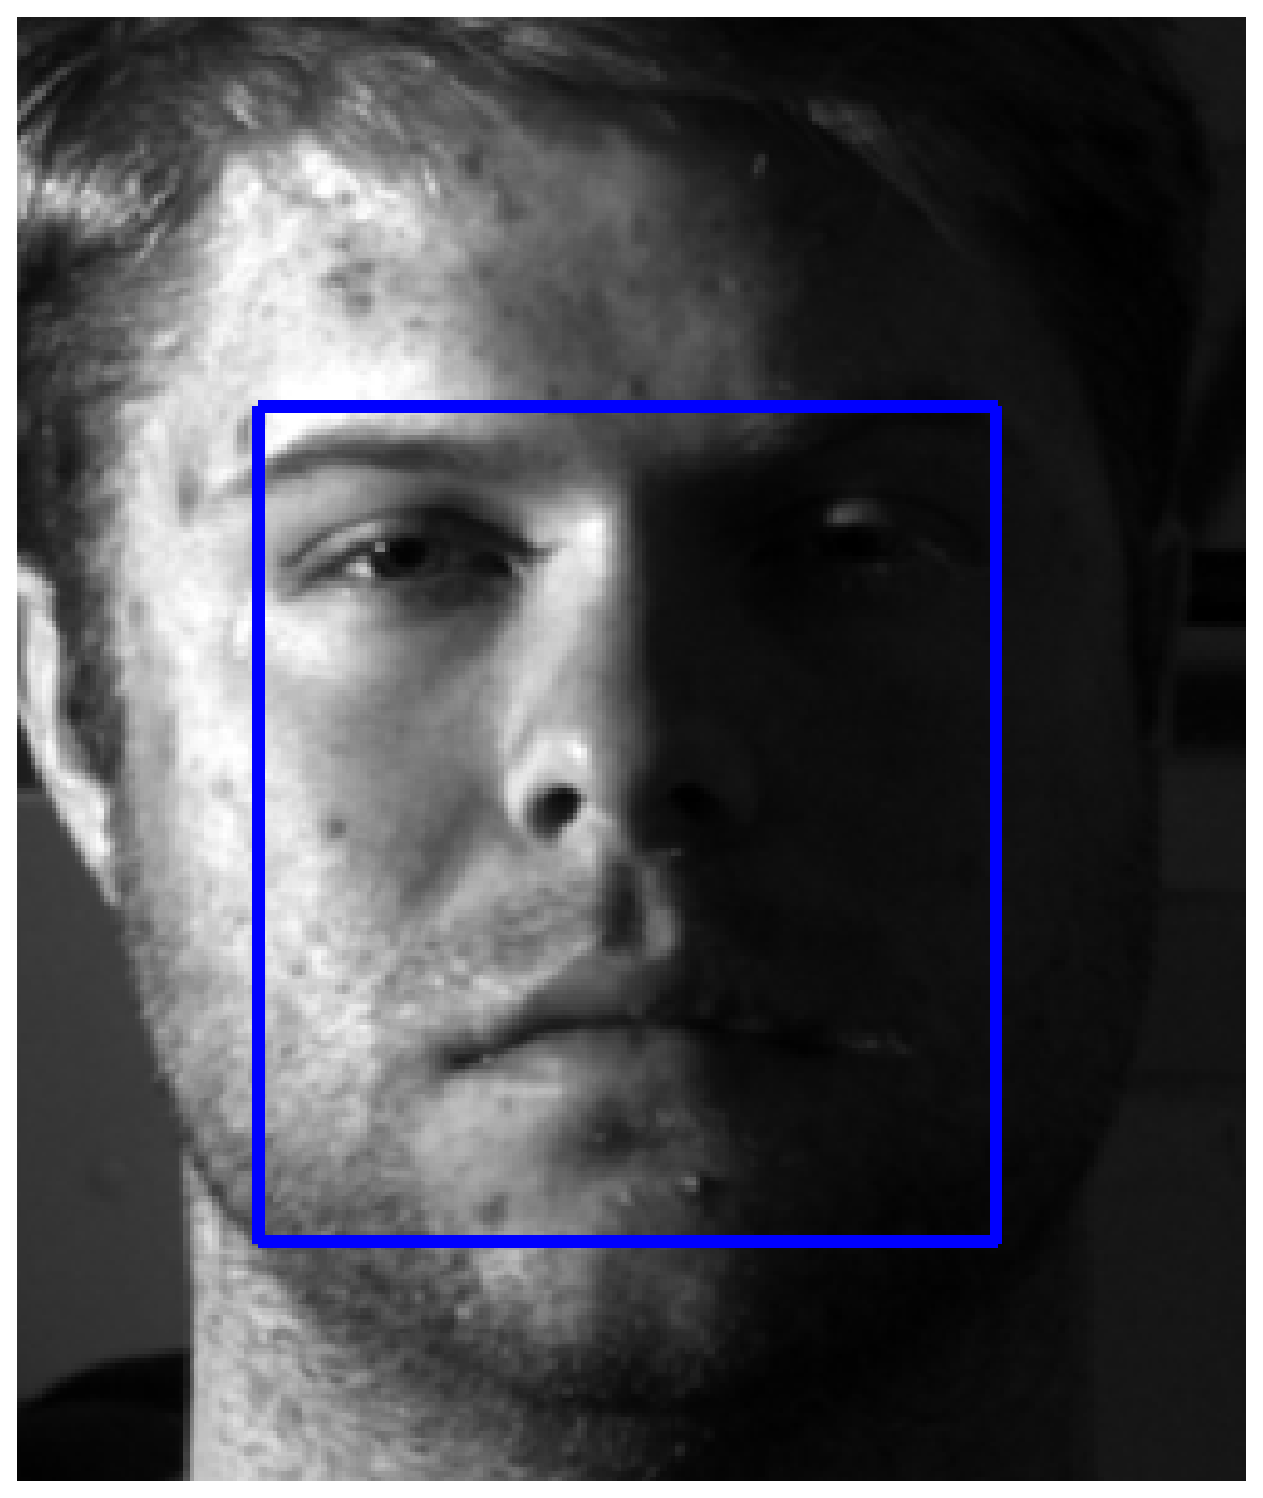
\includegraphics[width=0.18\linewidth]{figures/feature_based_aam/3_YaleB/1d}
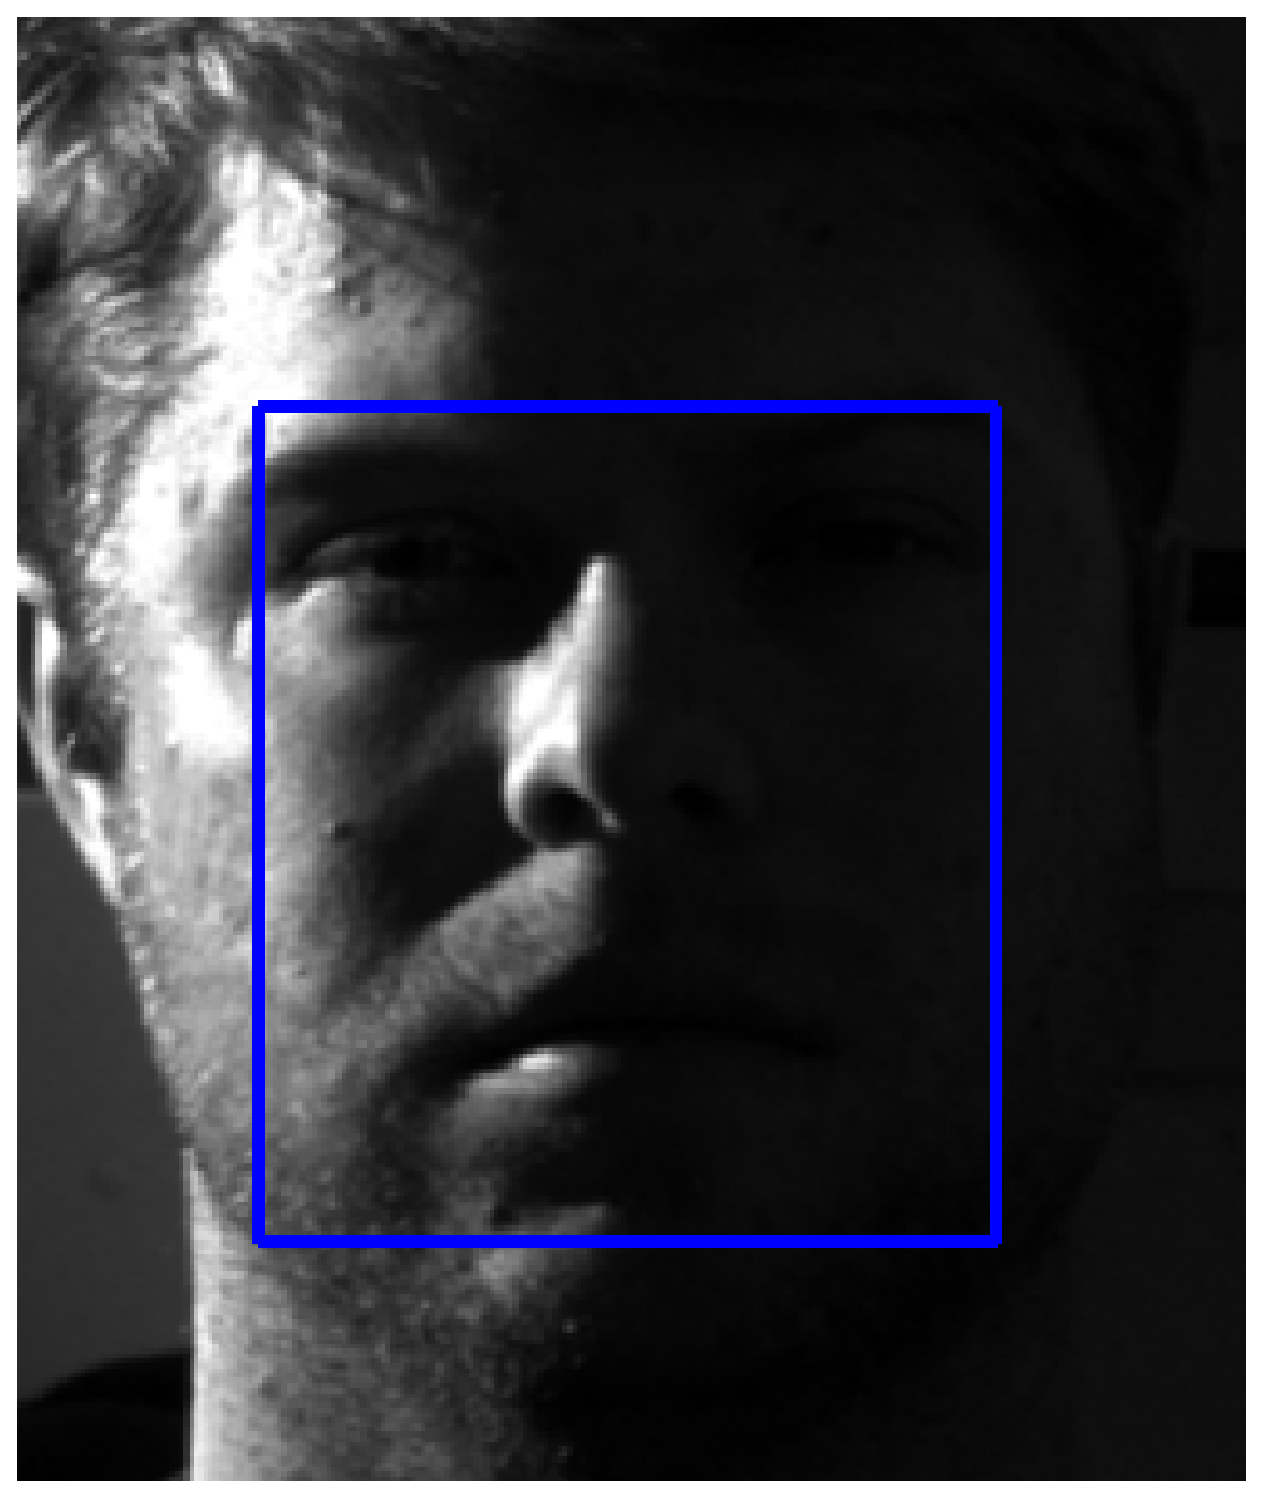
\includegraphics[width=0.18\linewidth]{figures/feature_based_aam/3_YaleB/1e}\\\vspace{0.1cm}
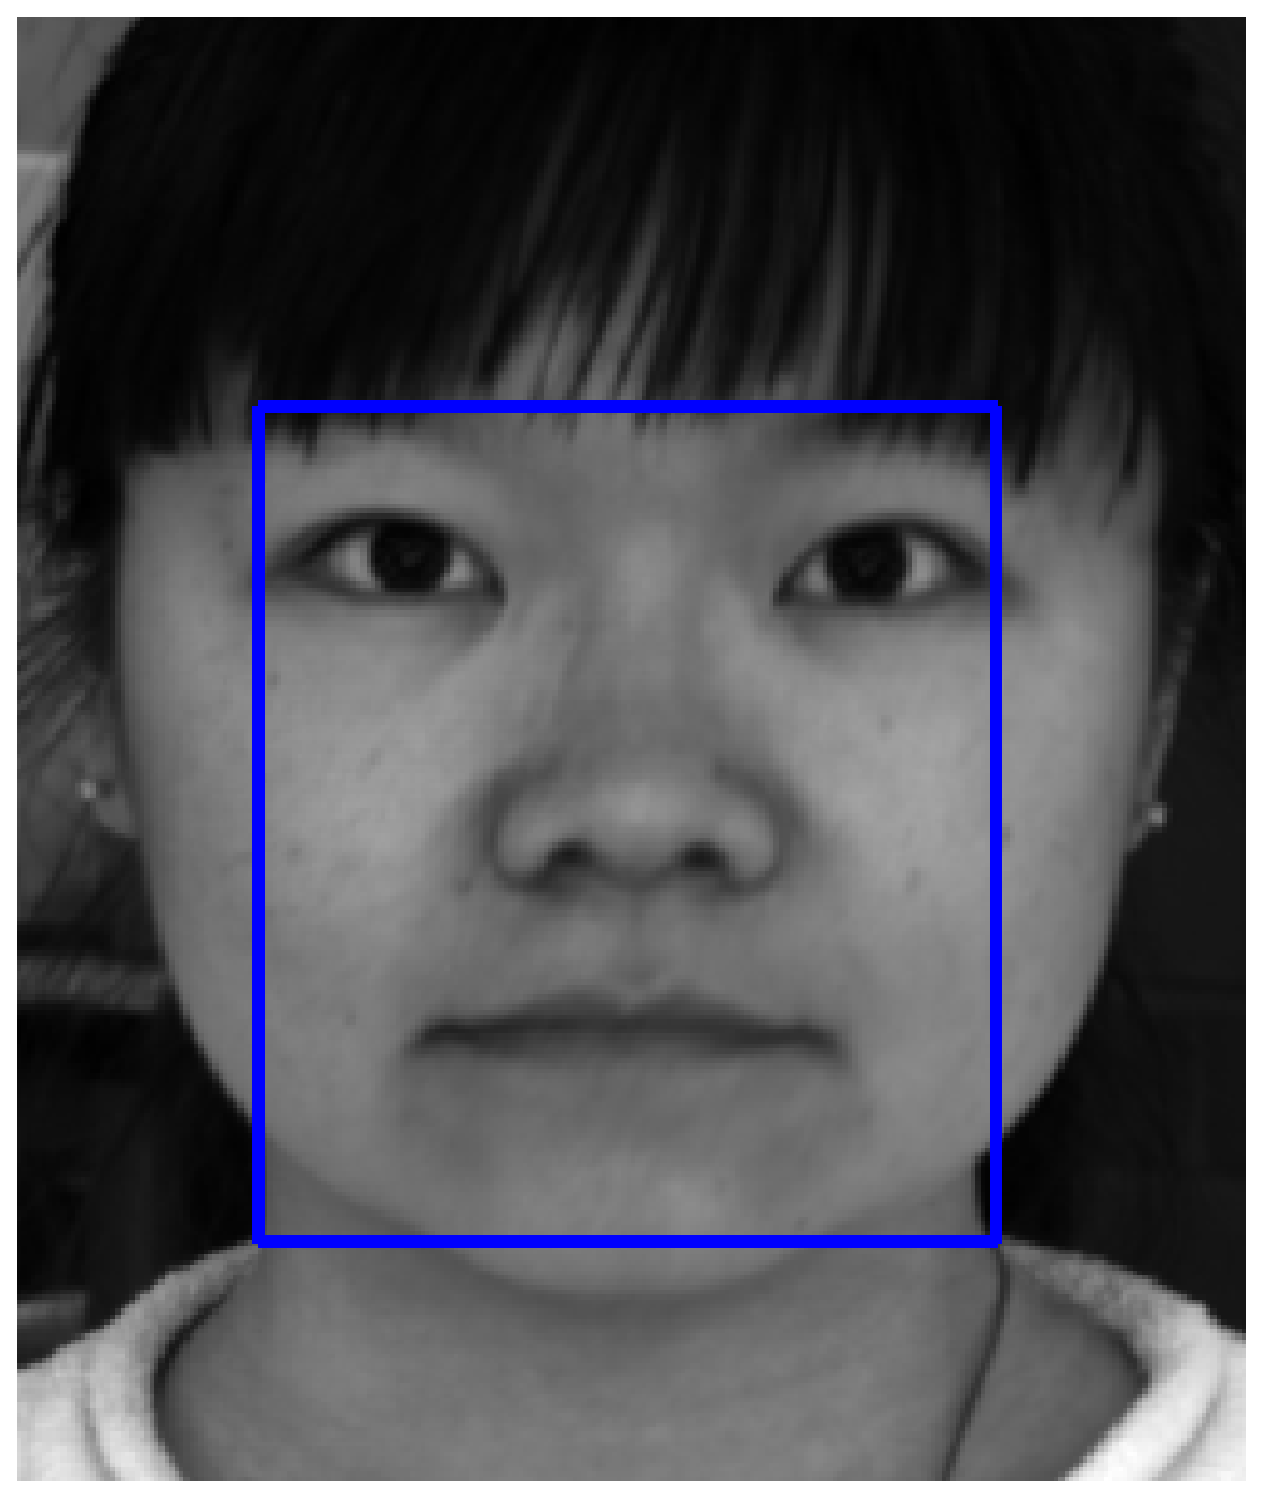
\includegraphics[width=0.18\linewidth]{figures/feature_based_aam/3_YaleB/2a}\hspace{0.4cm}
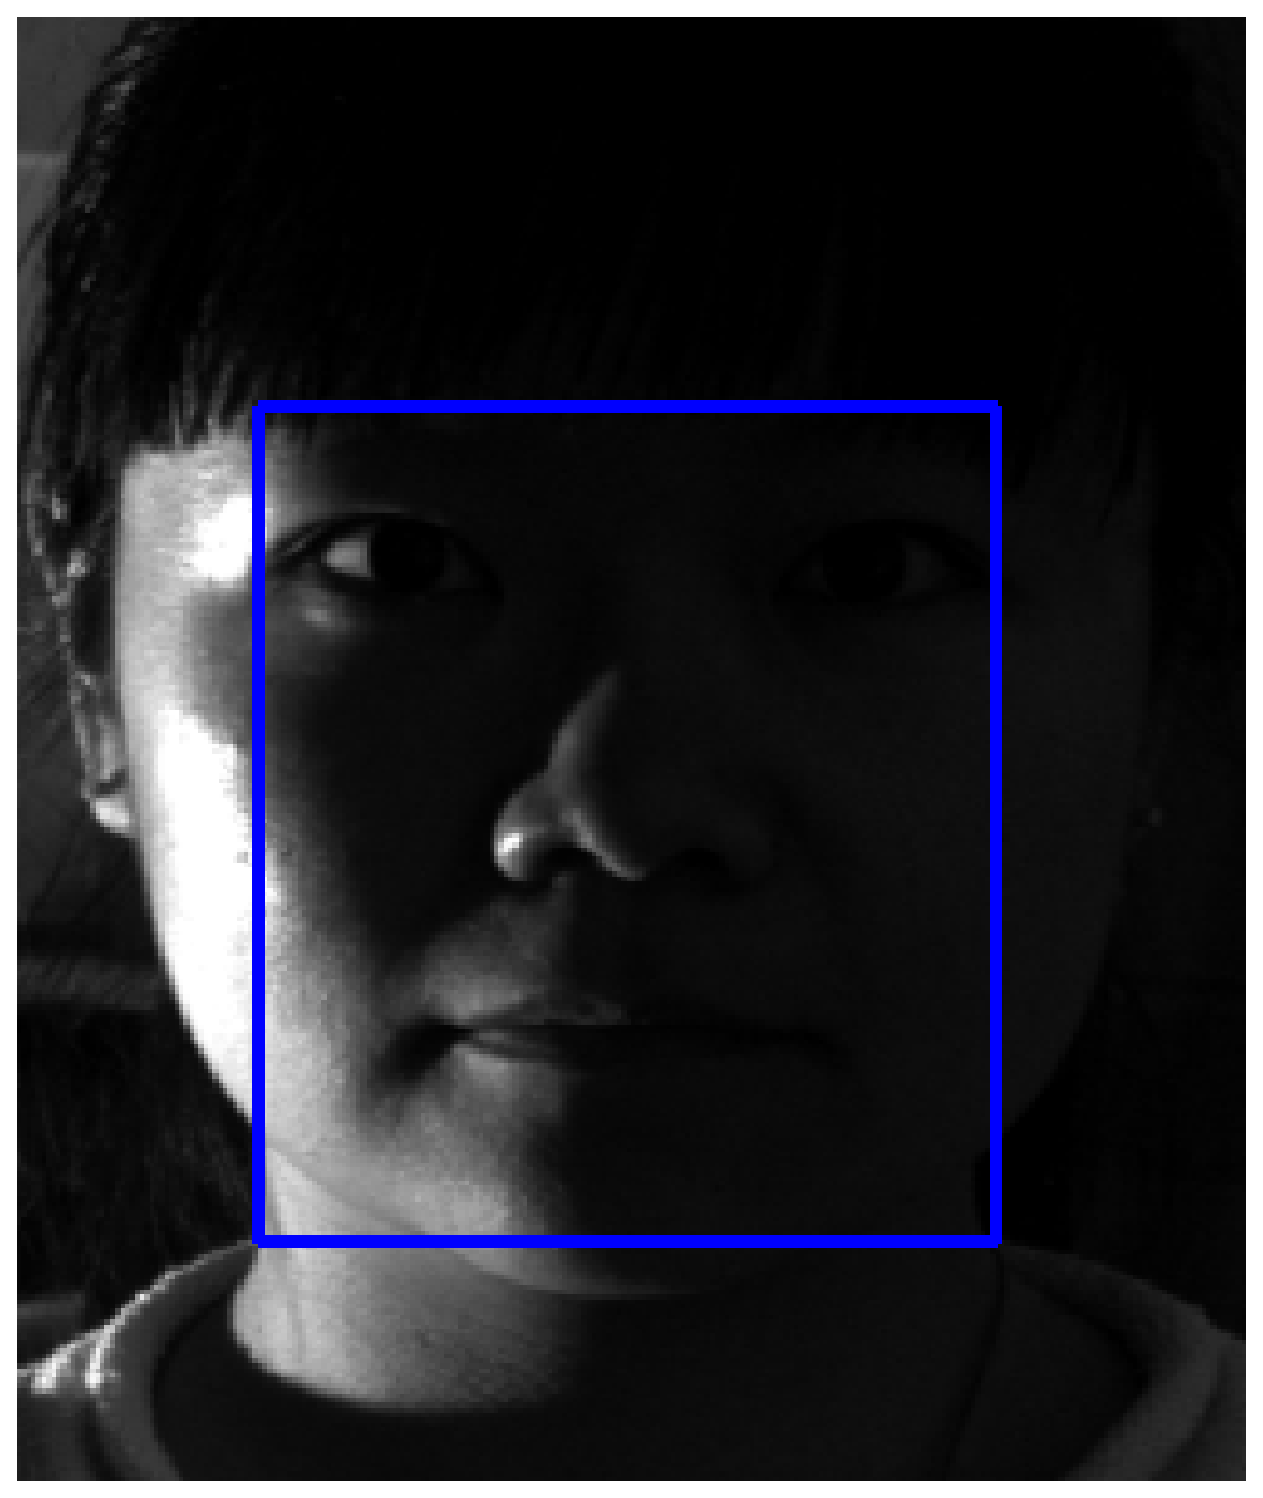
\includegraphics[width=0.18\linewidth]{figures/feature_based_aam/3_YaleB/2f}
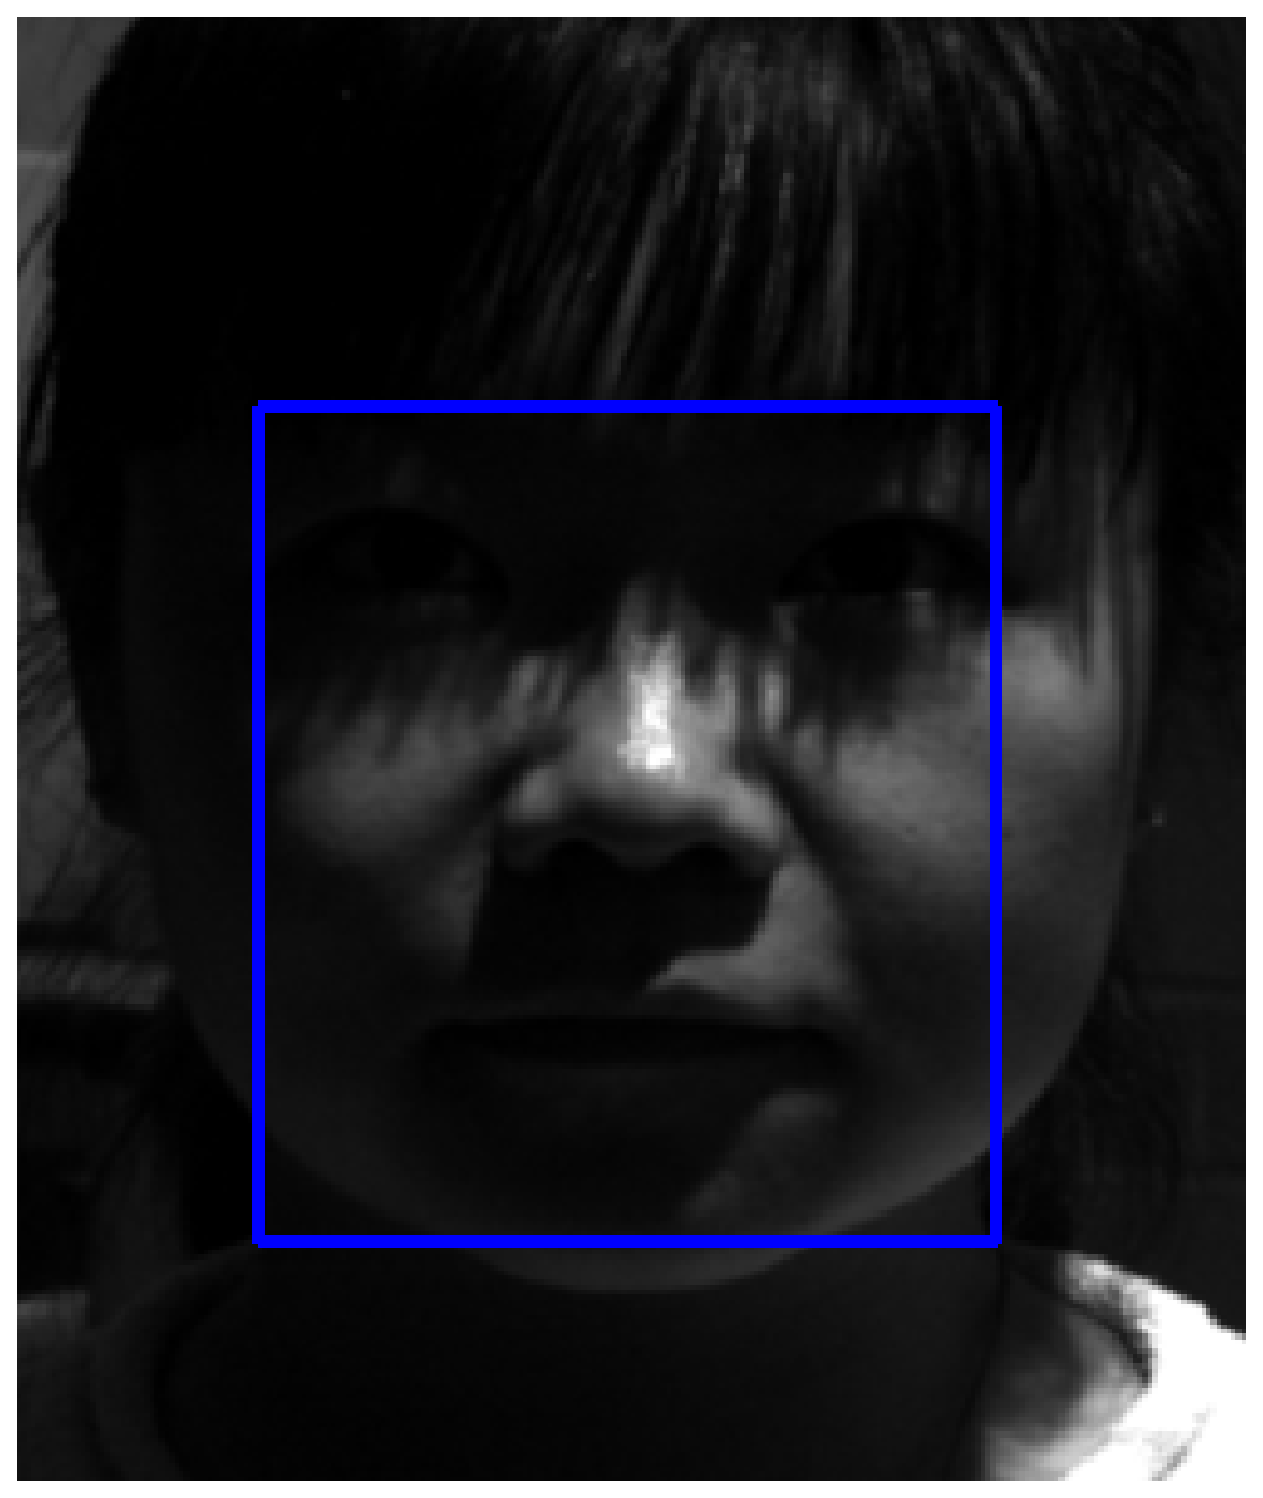
\includegraphics[width=0.18\linewidth]{figures/feature_based_aam/3_YaleB/2g}
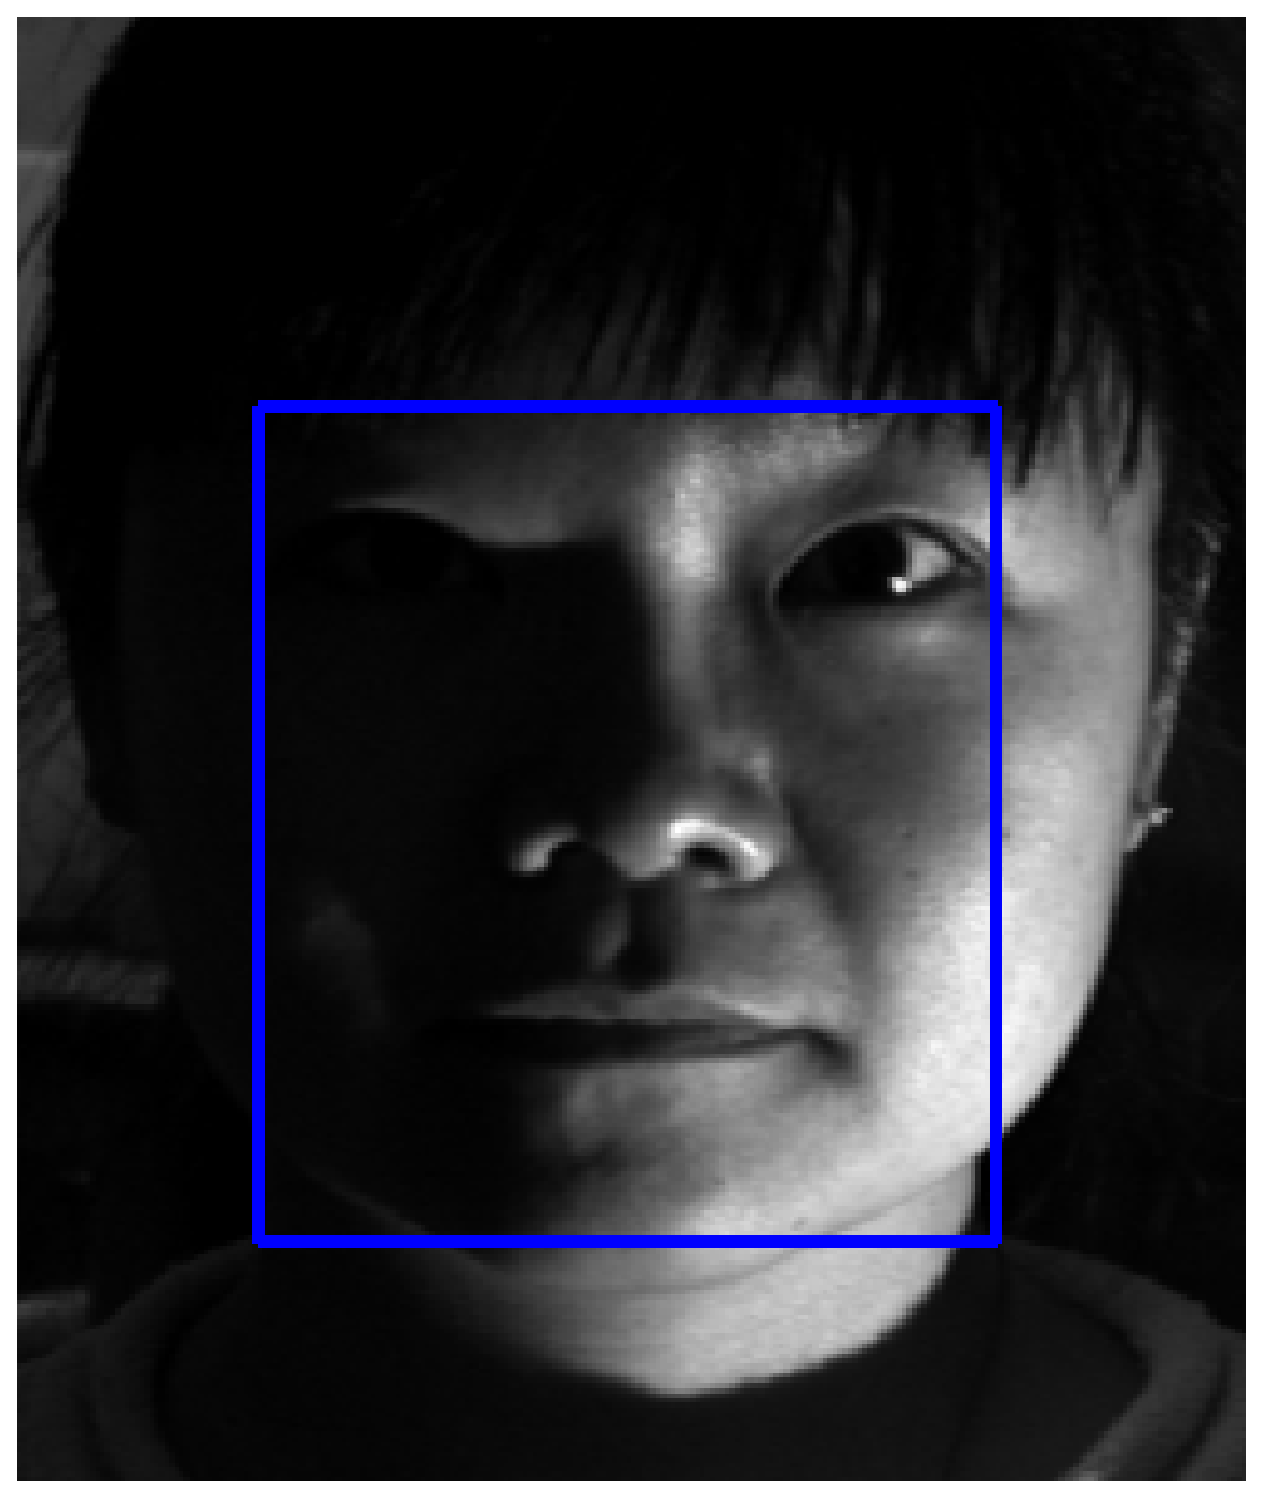
\includegraphics[width=0.18\linewidth]{figures/feature_based_aam/3_YaleB/2i}
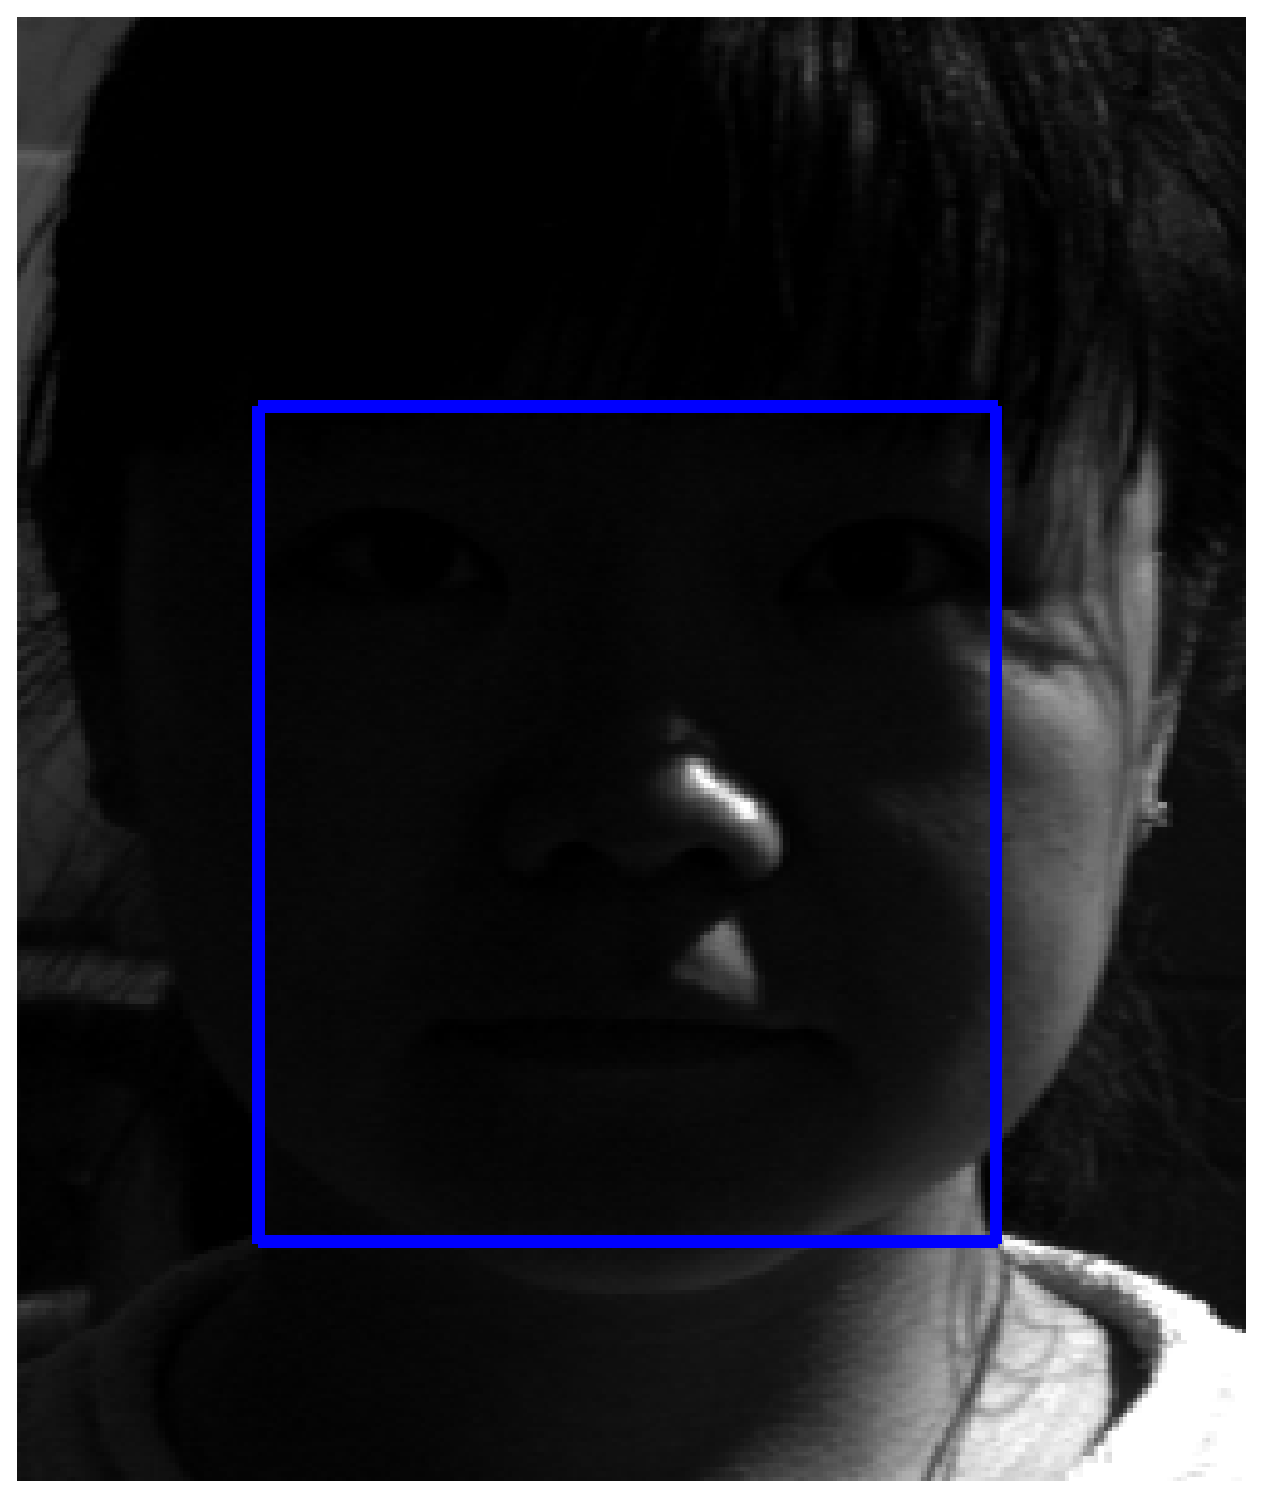
\includegraphics[width=0.18\linewidth]{figures/feature_based_aam/3_YaleB/2k}
\caption{Yale B Database images examples. The template image (left) is corrupted with extreme illumination in
the testing images for each subject.}
\label{fig:faceAlignment:images}
\end{figure}
%

%%%%%%%%%%%%%%%%%%%%%%%%%%%%%%%%%%%%%%%%%%%%%%%%%%%%%%%%%%%%%%%%%%%%%%%%%%%%%%%%%%%%%%%%%%%%%%% E X P E R I M E N T A L   R E S U L T S  :   L K %%%%%%%%%%%%%%%
%%%%%%%%%%%%%%%%%%%%%%%%%%%%%%%%%%%%%%%%%%%%%%%%%%%%%%%%%%%%%%%%%%%%%%%%%%%%%%%%
\subsection{Face Alignment (Lucas-Kanade)}\label{subsec:aam:faceAlignment}
In this section, we conduct experiments for the task of face alignment using
the LK-IC algorithm. In Sec.~\ref{subsec:aam:faceAlignment:comparison} we show a
motivating experiment in which we compare the performance of IC with warping
the features image at each iteration vs. extracting features from the warped
image. In Sec.~\ref{subsec:aam:faceAlignment:mainExperiment}, we compare the
performance of IC with warping the features image for all features types. For
both experiments, we use the Yale Face Database B~\cite{georghiades2001from},
which consists of 10 subjects with 576 images per subject under different
viewing conditions. We select 1 template image and 10 testing images for each
subject (100 image pairs) that are corrupted with extreme illumination
conditions (Fig.~\ref{fig:faceAlignment:images}).

We use the evaluation framework proposed in~\cite{baker2004lucas}. Specifically,
we define three canonical points within a region of interest for each image.
These points are randomly perturbed using a Gaussian distribution with standard
deviation $\sigma=\{1,2,\ldots,9\}$. Then, we create the affine distorted image
based on the affine warp defined between the original and perturbed points.
After applying 30 iterations of the IC optimization algorithm, we compute the
RMS error between the estimated and the correct locations of the three canonical
points. The optimization is considered to have converged if the final RMS error
is less than 3 pixels. Additionally, for each value of $\sigma$, we perform 100
experiments with different randomly perturbed warps. We evaluate the performance
by plotting the average frequency of convergence and the average mean RMS error
of the converged cases with respect to each value of $\sigma$. The results are
averaged over the 100 experiment repetitions with different random warps.

% Motivation figure
\begin{figure}[!h]
\centering
\hspace{0.50cm}
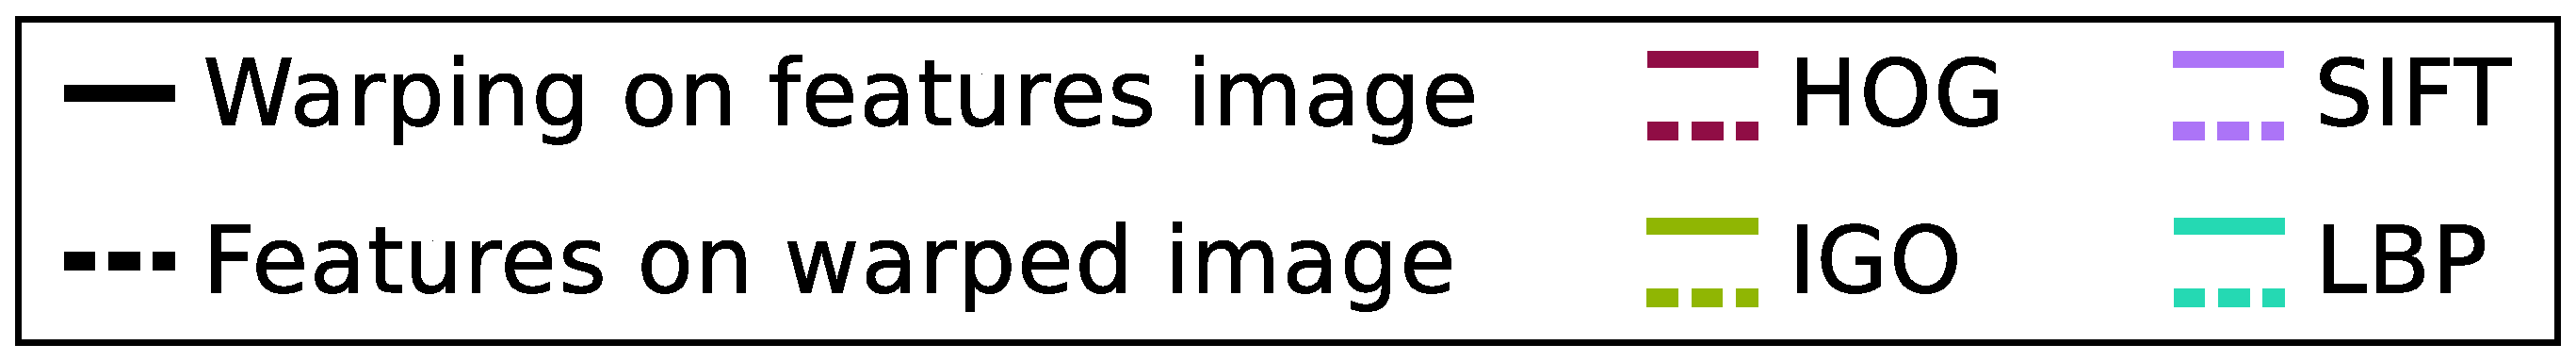
\includegraphics[height=0.90cm]{figures/feature_based_aam/4_CompositionDirectionsExperiment/legend}\\
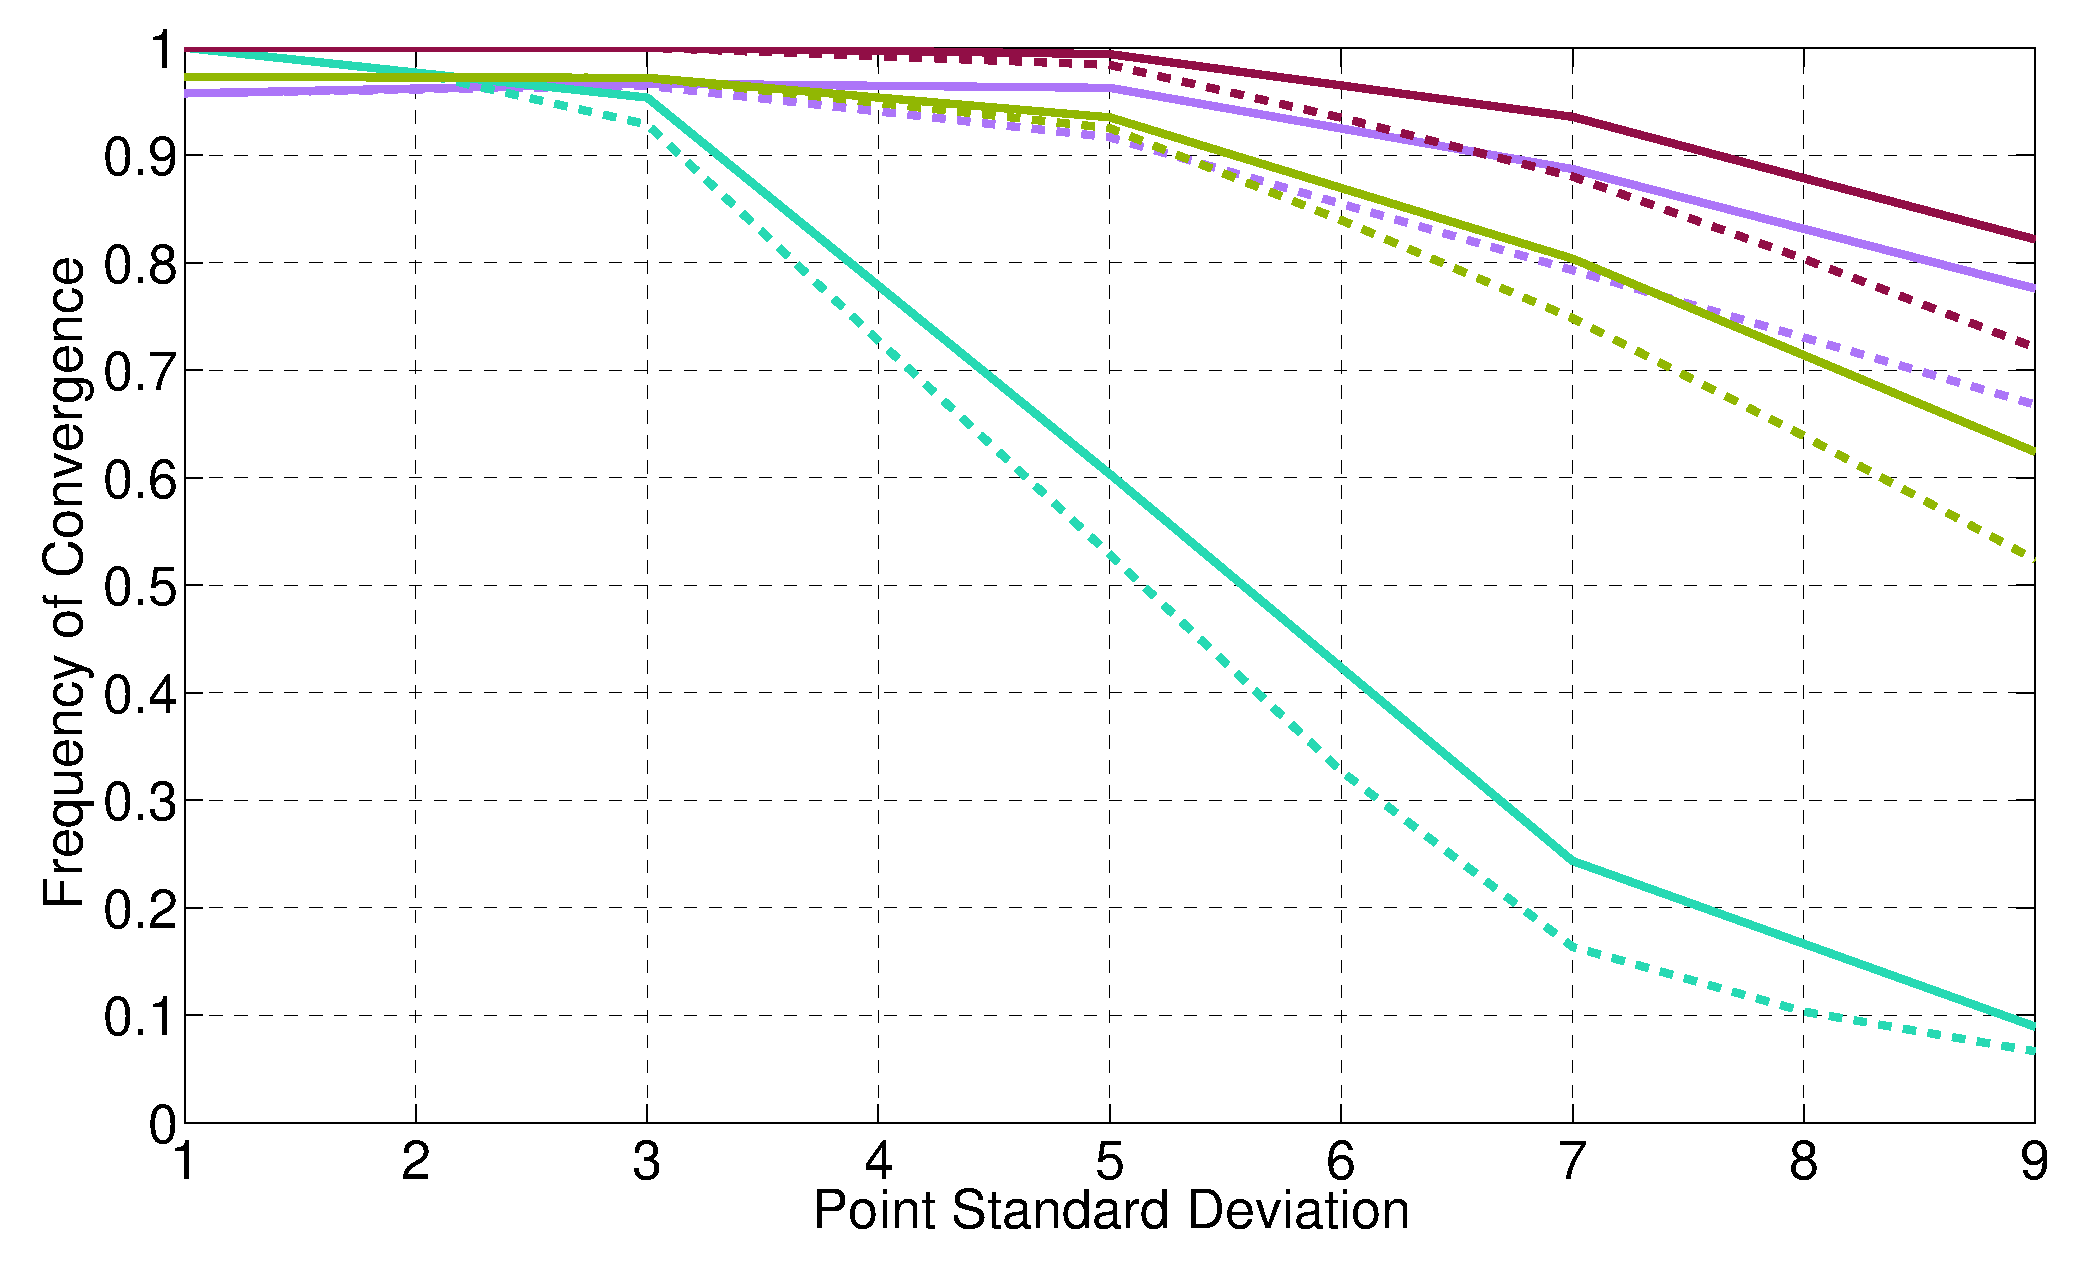
\includegraphics[width=0.70\linewidth]{figures/feature_based_aam/4_CompositionDirectionsExperiment/experiment}
\caption{Comparison between the techniques of warping the features image and
extracting features from the warped image. The plot shows results for HOG, SIFT,
IGO and LBP features, however the rest of the features demonstrate the same behaviour.}
\label{fig:warpFeaturesFeaturesWarpComparison}
\end{figure}
%
% Comparison
\subsubsection{Warping of features image vs Features from warped image}
\label{subsec:aam:faceAlignment:comparison}
In the experiment of Fig.~\ref{fig:warpFeaturesFeaturesWarpComparison} we compare
the performance of the two possible combination techniques between the features
extraction function and the warp function, as presented in
Sec.~\ref{sec:aam:featureBasedOptimization}. The figure shows only HOG, SIFT, IGO
and LBP cases, though we get the same results with the rest of features types.
The comparison indicates that the method of extracting the features from the
original image outperforms the one of extracting the features from the warped image,
especially for large values of $\sigma$. The reason behind this behavior is that
the warping of an image provokes some distortion on the texture which partly
destroys the local structure. This has negative consequences on the computation
of all the employed features, because the descriptor of each pixel depends on
the structure of its neighborhood.

% Main experiment
\subsubsection{Features Comparison}
\label{subsec:aam:faceAlignment:mainExperiment}
Figure~\ref{fig:faceAlignment} provides an evaluation of the robustness of each
feature by showing the average frequency of convergence with respect to each
value of $\sigma$. This experiment clearly indicates that Intensities or
Gabor Magnitude features are totally inappropriate for such a task. HOG is the
most robust feature with remarkable convergence frequency, followed by SIFT,
IGO and ES. Finally, the LBPs family and Gabor Angles are not robust, but they
can achieve decent results when the initialization is good.

% LK Accuracy
\begin{figure}[!h]
\centering
\hspace{0.52cm}\includegraphics[height=0.90cm]{figures/feature_based_aam/5_LKaccuracy/legend}\\
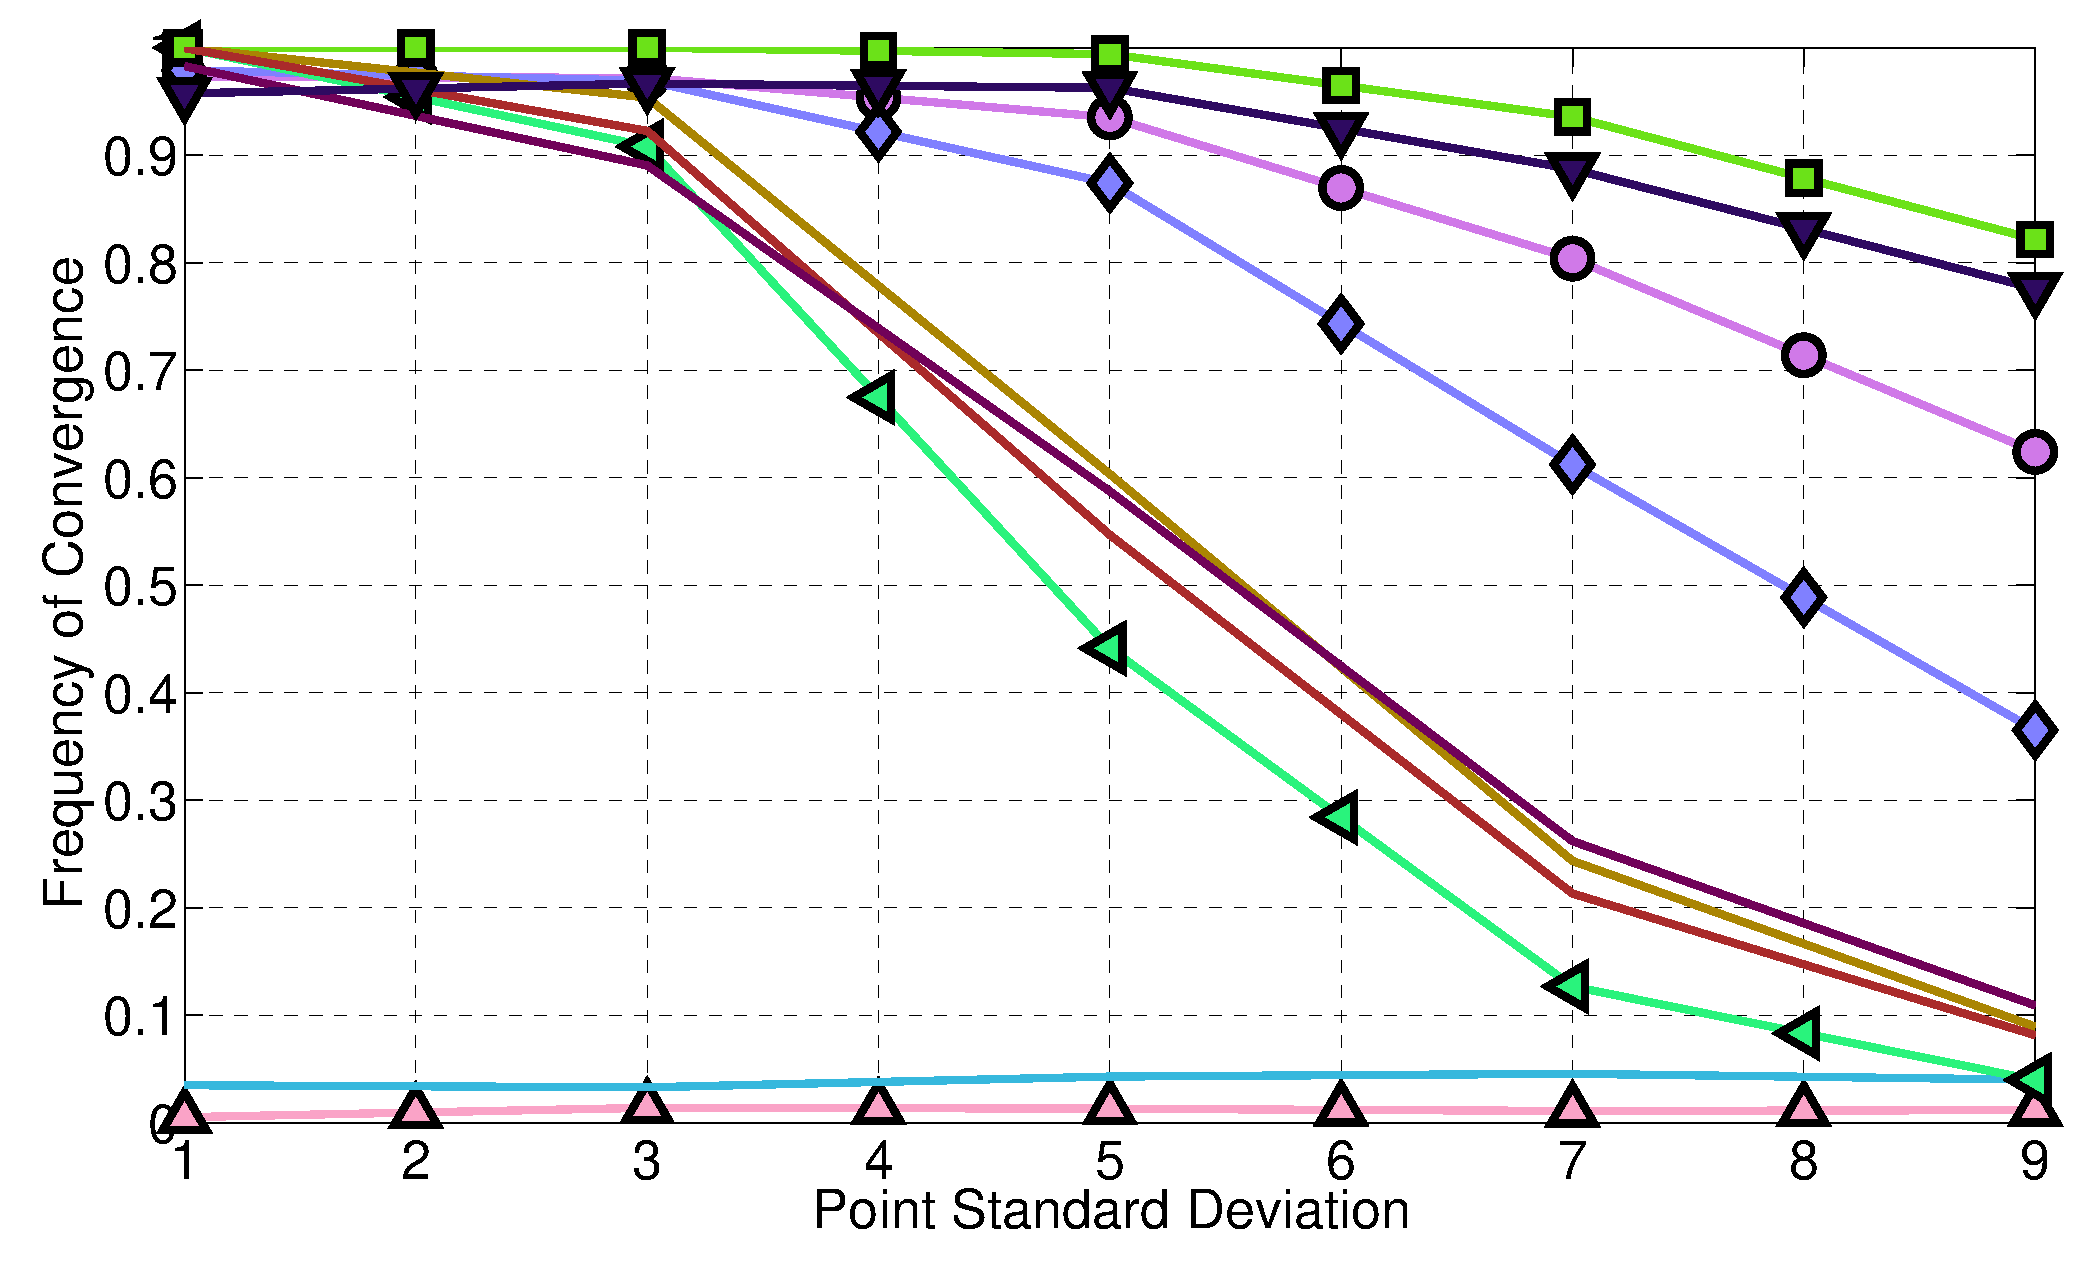
\includegraphics[width=0.70\linewidth]{figures/feature_based_aam/5_LKaccuracy/experiment}\label{fig:faceAlignment}
\caption{Face alignment (Lucas-Kanade) results on Yale B database using the
inverse compositional framework. The figure shows the frequency of convergence
with respect to the standard deviation $\sigma$.}
\label{fig:faceAlignment}
\end{figure}
%



%%%%%%%%%%%%%%%%%%%%%%%%%%%%%%%%%%%%%%%%%%%%%%%%%%%%%%%%%%%%%%%%%%%%%%%%%%%%%%%%
%%%%%%%%%%%%% E X P E R I M E N T A L   R E S U L T S  :   A A M s %%%%%%%%%%%%%
%%%%%%%%%%%%%%%%%%%%%%%%%%%%%%%%%%%%%%%%%%%%%%%%%%%%%%%%%%%%%%%%%%%%%%%%%%%%%%%%
\subsection{Face Fitting (Active Appearance Models)}
\label{subsec:aam:AAMs}
In this section we compare the performance of the selected features using AAMs
for the task of face fitting with cross-database experiments. We investigate
\emph{which} features are more suitable for the task by comparing them with
respect to their accuracy (Sec.~\ref{sec:aam:accuracy}), speed of convergence
(Sec.~\ref{sec:aam:convergence}) and computational cost
(Sec.~\ref{sec:aam:timings}). We also shed light on \emph{why} some features
perform better by comparing them with respect to the number of appearance
components (Sec.~\ref{sec:aam:n_components}), the neighborhood size per pixel
(Sec.~\ref{sec:aam:neighbourhood}) and the smoothness of their cost function
(Sec.~\ref{sec:aam:cost_function}).

As explained in Sec.\ref{subsec:aam:inverseCompositional:alternating}, AIC and
SIC algorithms are theoretically equivalent and the only difference between
them is that SIC is significantly slower. Specifically, the updates of SIC
(Eq.~\ref{equ:sicUpdate}) and AIC (Eqs.~\ref{equ:aicUpdate1} and
\ref{equ:aicUpdate2}) are theoretically guaranteed to be the
same~\cite{tzimiropoulos2013optimization}. Thus, herein we employ the AIC and
POIC algorithms.

We use the in-the-wild databases presented in
Sec.~\ref{sec:notation:databases}. Specifically, we use the 811 image of the
LFPW trainset~\cite{belhumeur2011localizing} for training. The testing is
performed on AFW~\cite{zhu2012face}, LFPW testing
set~\cite{belhumeur2011localizing}, Helen training and testing
set~\cite{le2012interactive} and iBUG~\cite{sagonas2013semi}, thus 3026
in-the-wild images in total. The fitting process is always initialized by
computing the face's bounding box using Cascade Deformable Part Models (CDPM)
face detector~\cite{orozco2013empirical}. The fitting error is computed with
the RMSE of Eq.~\ref{equ:error} normalized with the face size of
Eq.~\ref{equ:error_normalization}.

% AAMs Accuracy
\begin{figure}[!t]
\centering
\hspace{0.5cm}\includegraphics[height=0.90cm]{figures/feature_based_aam/6_AAMaccuracy/legend}\\
\subfloat[Alternating IC]{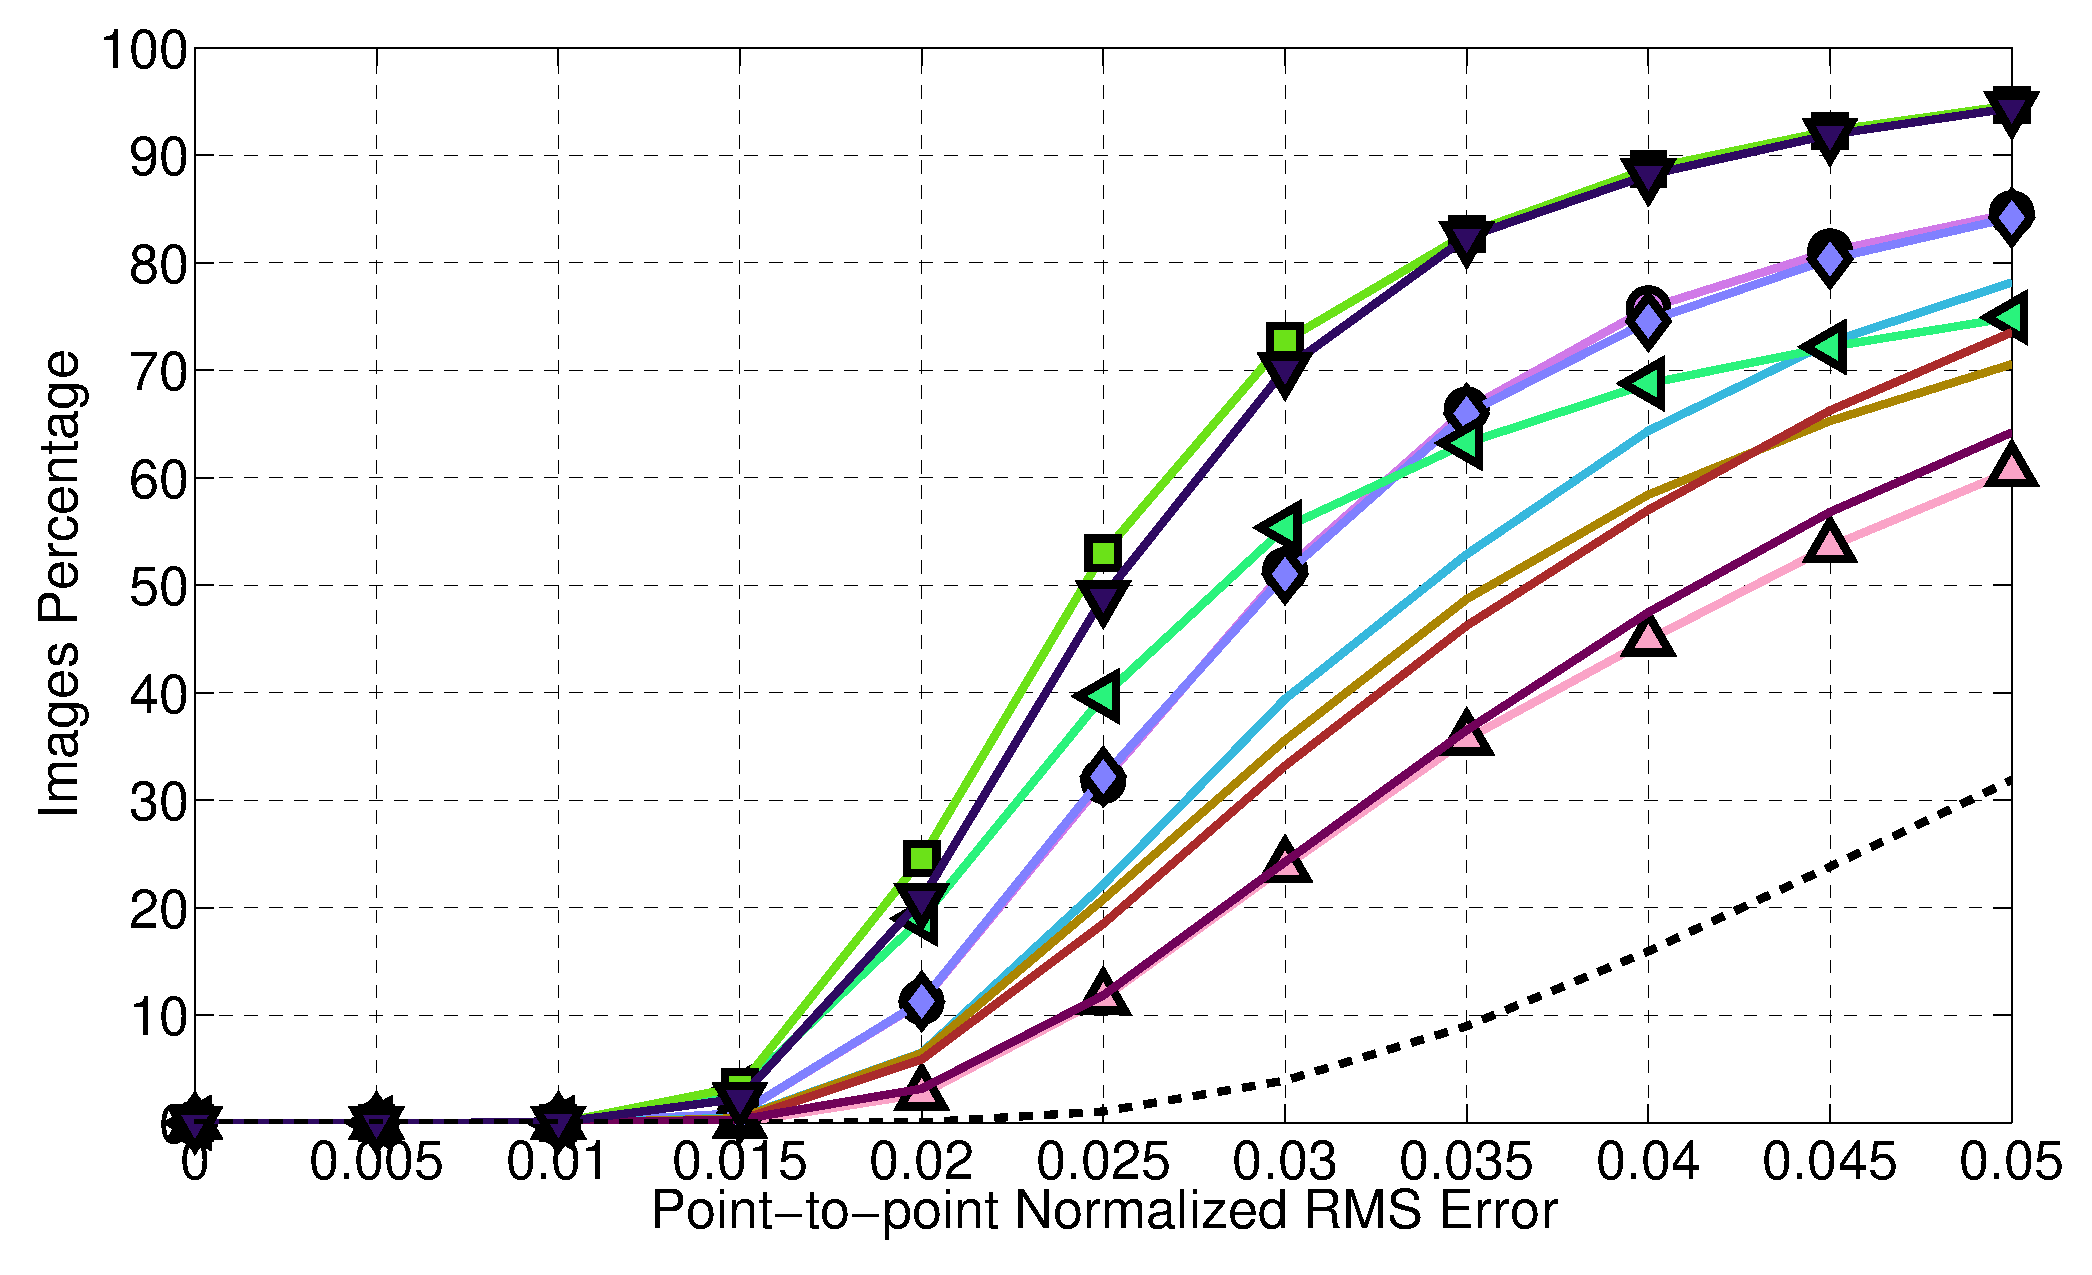
\includegraphics[width=0.70\linewidth]{figures/feature_based_aam/6_AAMaccuracy/alternating}\label{fig:faceFitting:alternating}}\\
\subfloat[Project-Out IC]{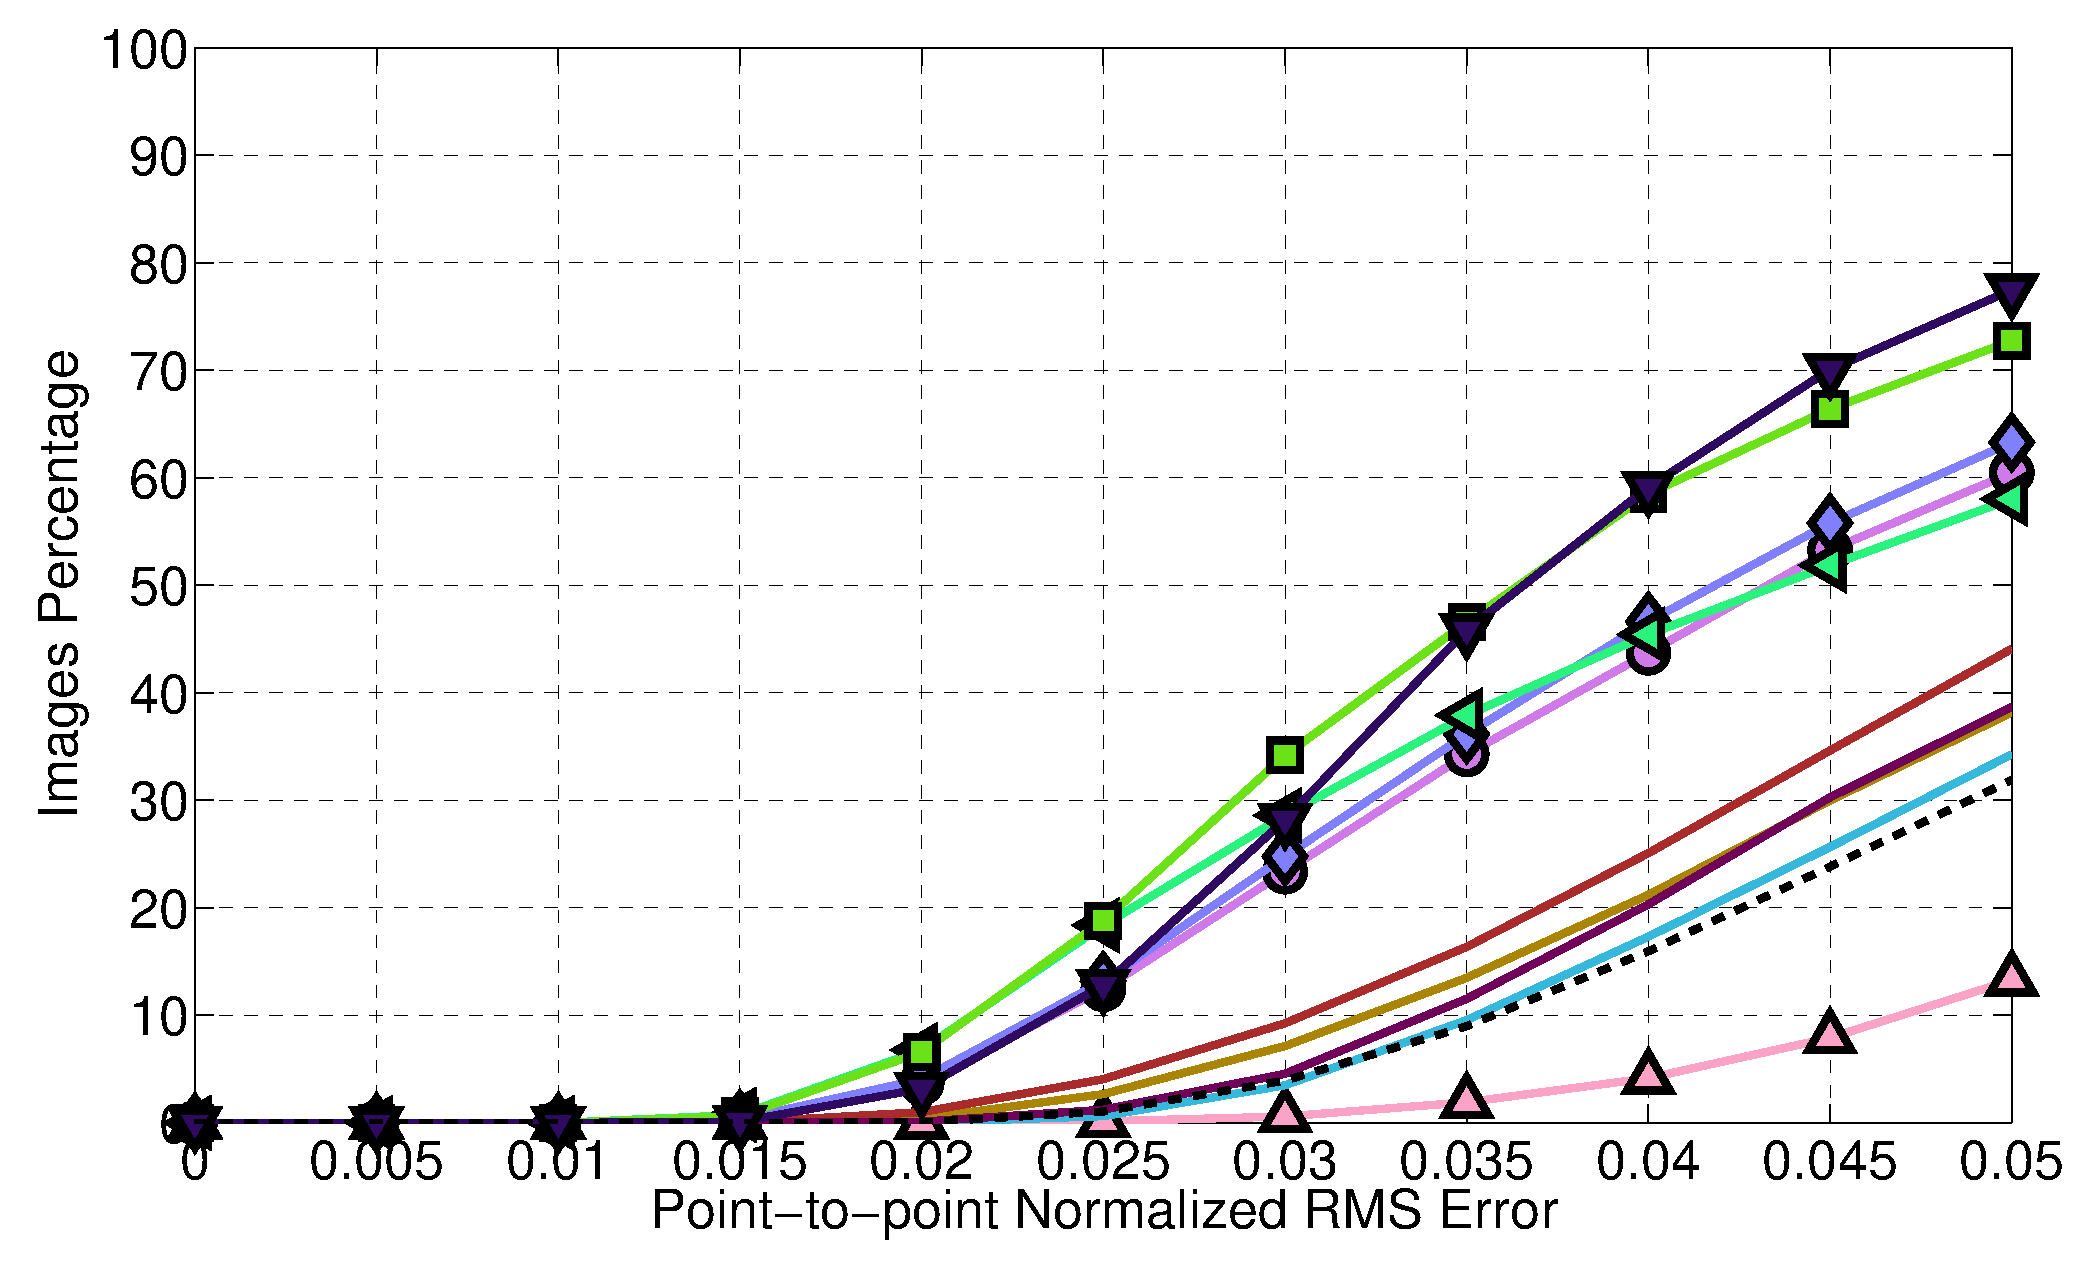
\includegraphics[width=0.70\linewidth]{figures/feature_based_aam/6_AAMaccuracy/project-out}\label{fig:faceFitting:project-out}}
\caption{Face fitting (AAMs) accuracy on in-the-wild databases (3026 test images) using the alternating and project-out inverse compositional frameworks, evaluated on 68 landmark points.}
\label{fig:faceFitting}
\end{figure}
%

% Accuracy
\subsubsection{Accuracy}\label{sec:aam:accuracy}
Figures~\ref{fig:faceFitting:alternating} and \ref{fig:faceFitting:project-out}
compare the accuracy of AIC and POIC respectively on all the databases
(3026 testing images) for all the features types. The fitting procedure is
performed using the methodology of Sec.~\ref{sec:aam:featuresThenWarp} and keeping
$n_s=15$ eigenshapes and $n_a=100$ eigentextures, regardless of the feature type.
The results are plotted in the form of Cumulative Error Distributions (CED).
Note that this experiment intends to make a fair comparison of the accuracy
between the various features by letting the fitting procedure converge for all feature
types. The results indicate that HOG and SIFT features are the most appropriate
for the task. HOG features perform better in the case of AIC and the SIFT ones
are more robust for POIC, however the differences between them are very small.
IGO and ES features have a sufficiently good performance. Moreover, similar to
the face alignment case, Gabor Angles are not robust, but they achieve very accurate
fitting result when they converge, especially in the POIC case. On the contrary,
even though Gabor Magnitude features demonstrate a decent performance in the AIC,
they completely diverge in the POIC case. This observation, combined with their
performance with the LK algorithm, indicates that they are unsuitable for image
alignment without a linear appearance variation model. The same fact stands for
intensities as well. Finally, the LBPs family has relatively poor performance.
Figure~\ref{fig:afw-helen-images} shows some indicative fitting examples from
the very challenging iBUG database for all features with AIC.


% Convergence
\subsubsection{Convergence}\label{sec:aam:convergence}
Herein, we examine the frequency of convergence achieved by each feature type.
We assume that a fitting procedure has converged when either the cost function
error incremental or the landmarks mean displacement are very small.

% AAMs Convergence
\begin{figure}[!h]
\centering
\hspace{0.3cm}\includegraphics[height=0.90cm]{figures/feature_based_aam/7_AAMconvergence/legend}\\
\subfloat[Alternating IC]{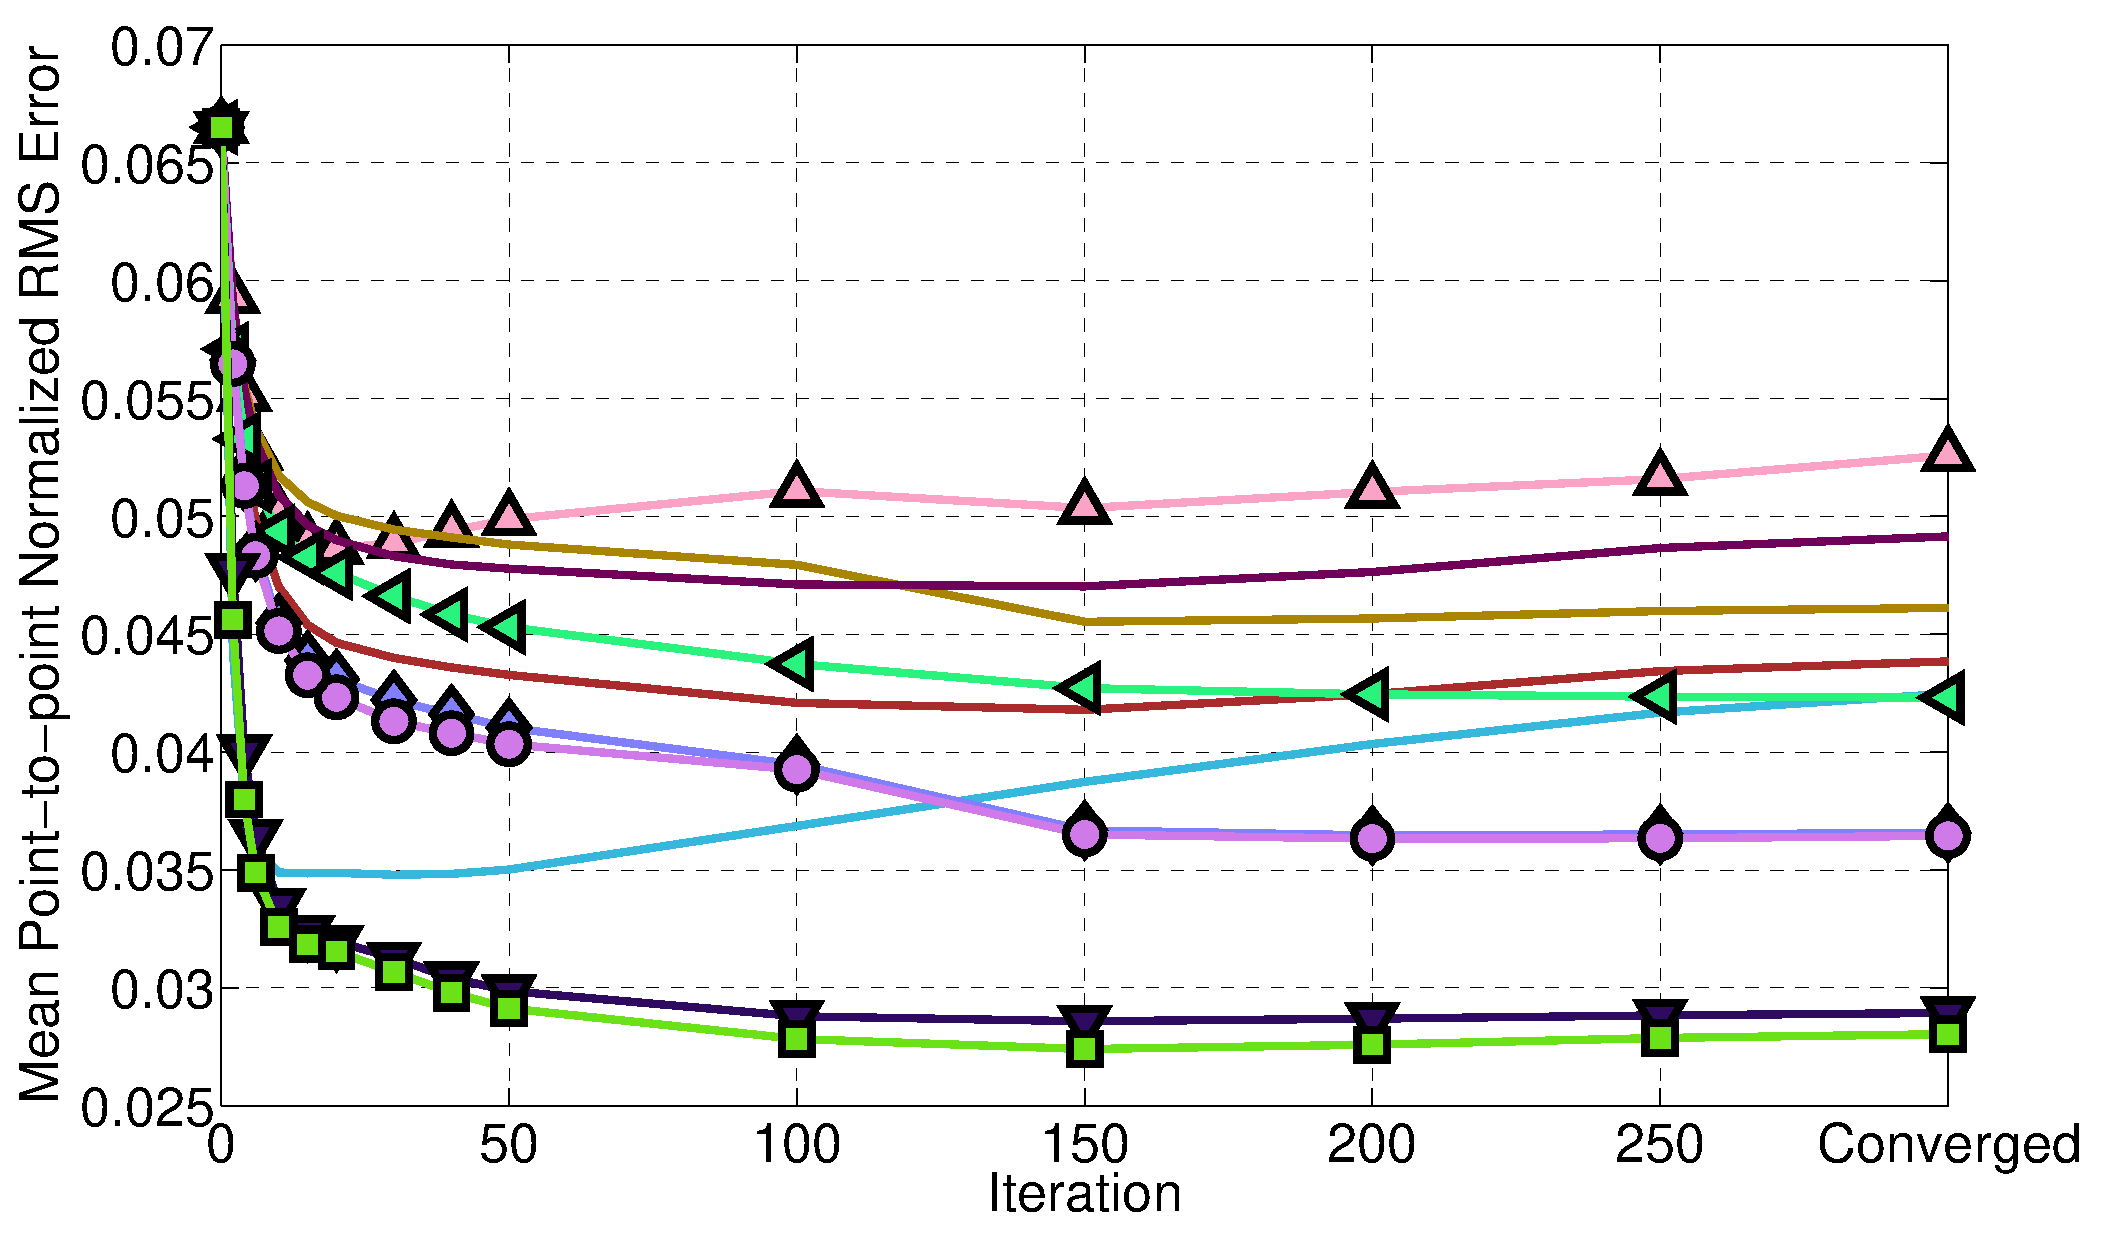
\includegraphics[width=0.70\linewidth]{figures/feature_based_aam/7_AAMconvergence/alternating}\label{fig:convergence:alternating}}\\
\subfloat[Project-Out IC]{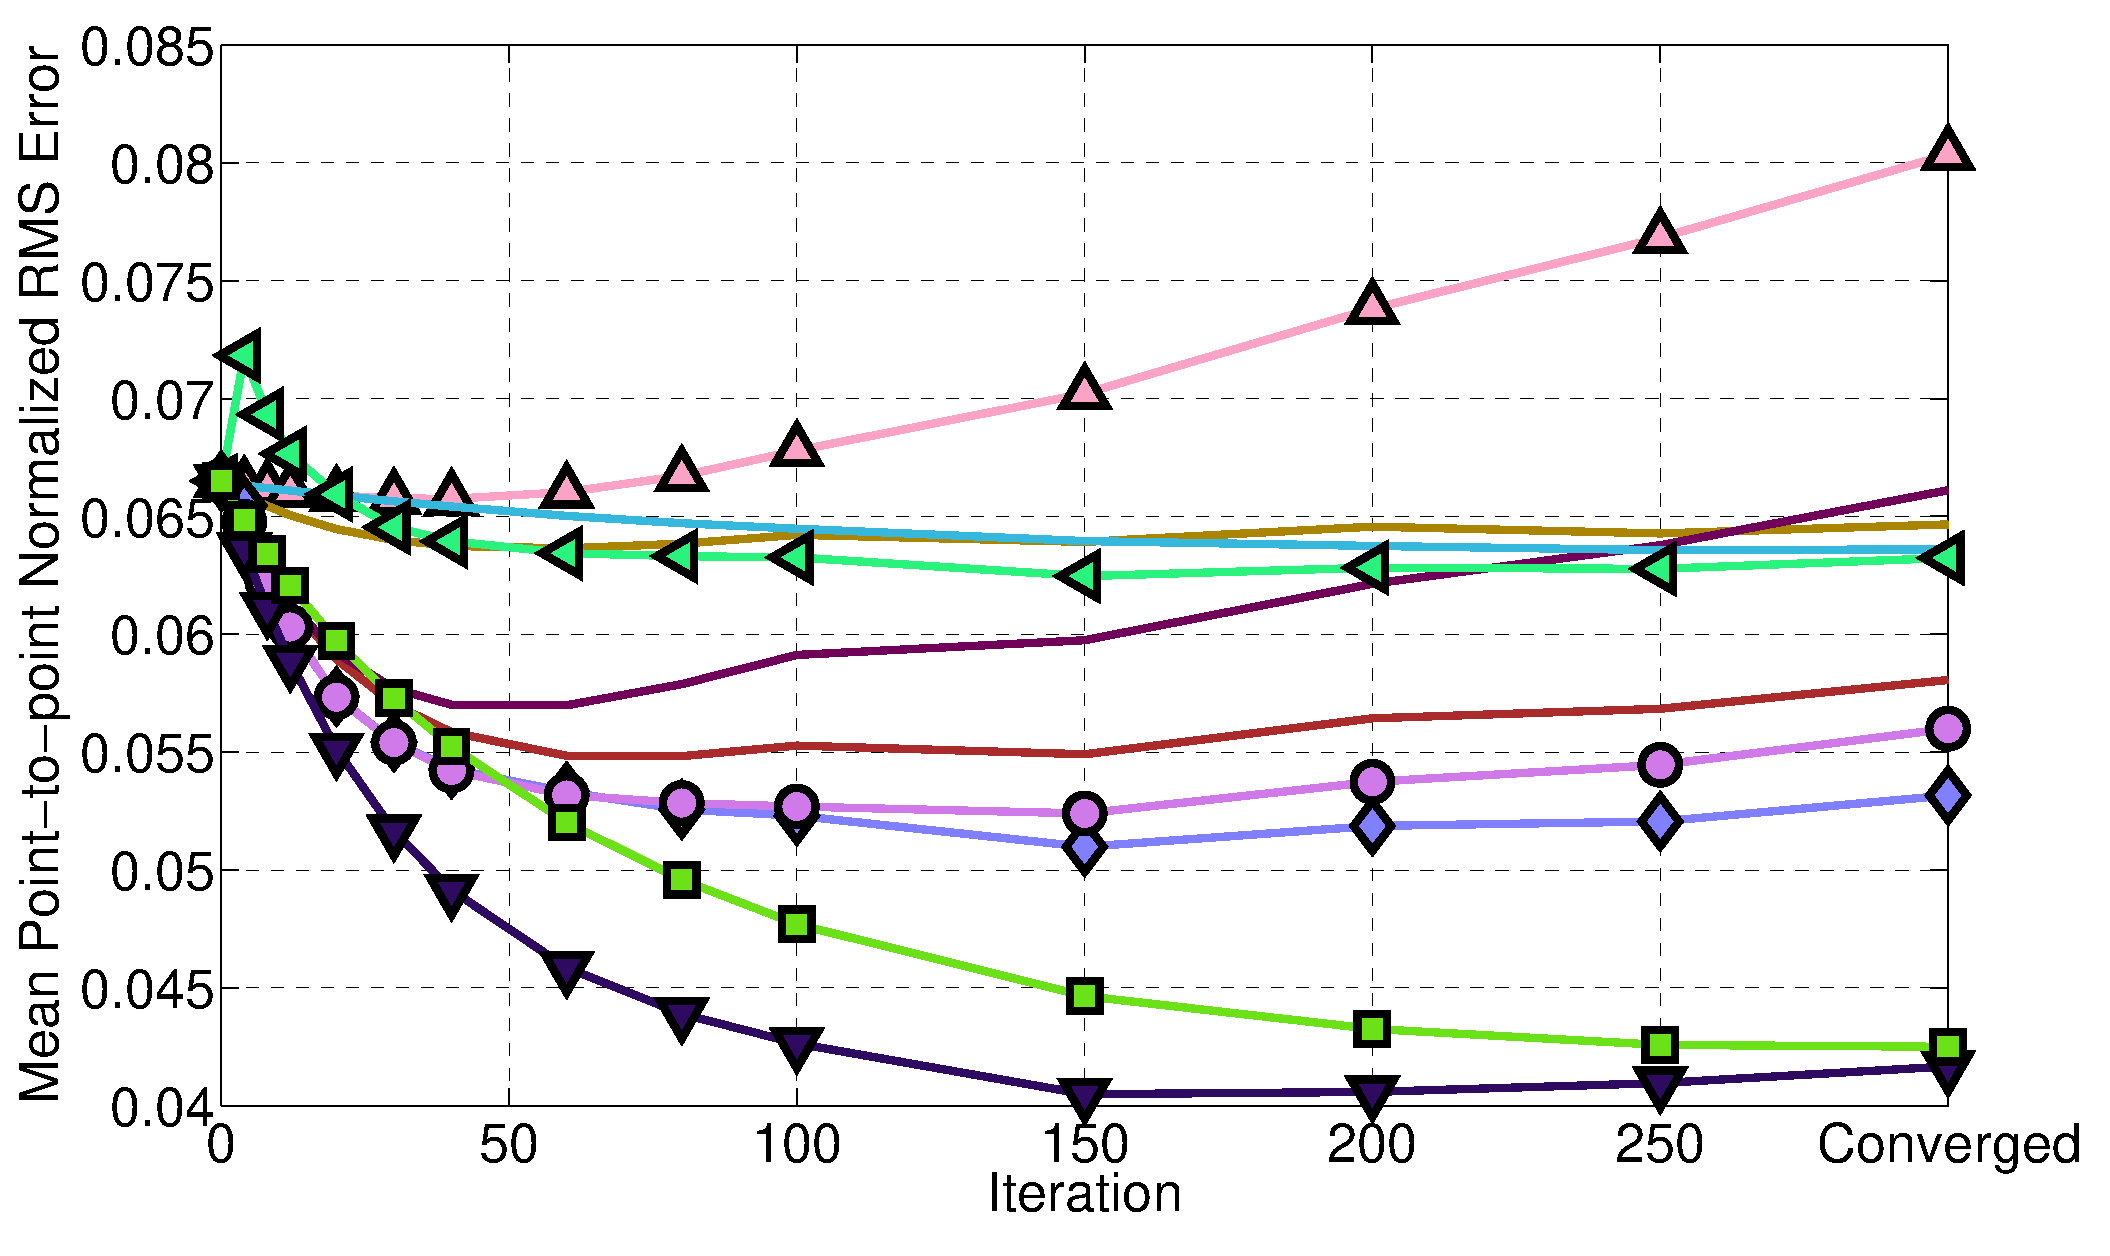
\includegraphics[width=0.70\linewidth]{figures/feature_based_aam/7_AAMconvergence/project_out}\label{fig:convergence:project-out}}
\caption{Mean point-to-point normalized RMS fitting error with respect to
iteration number on in-the-wild databases (3026 test images). The plot aims to
compare the speed of convergence of each feature type. Please refer to
Table~\ref{tab:times} (columns 5-10) for the computational cost of each
feature-based method.}
\label{fig:feature_aam:convergence}
\end{figure}
%

The cost incremental criterion is defined as
%%%%%%%%%%%%%%
\begin{equation}
  \frac{abs(error_{k-1}-error_{k})}{error_{k-1}}<\epsilon
\end{equation}
%%%%%%%%%%%%%%
where $error_k$ is the cost function error from
Eq.~\ref{equ:minimizationCostForAAMs} at current iteration $k$ and
$\epsilon=10^{-5}$. The mean displacement criterion is defined as the mean
point-to-point normalized Euclidean distance between the shapes of current and
previous iterations, thus
%%%%%%%%%%%%%%
\begin{equation}
  \frac{\sum_{i=1}^n\sqrt{(x_i^k-x_i^{k-1})^2+(y_i^k-y_i^{k-1})^2}}{cn} < \epsilon
\end{equation}
%%%%%%%%%%%%%%
with $\epsilon=10^{-4}$.

% Speed of Convergence
\begin{figure}[!h]
\centering
\hspace{0.4cm}\includegraphics[height=0.90cm]{figures/feature_based_aam/8_AAMconvergenceSpeed/legend}\\
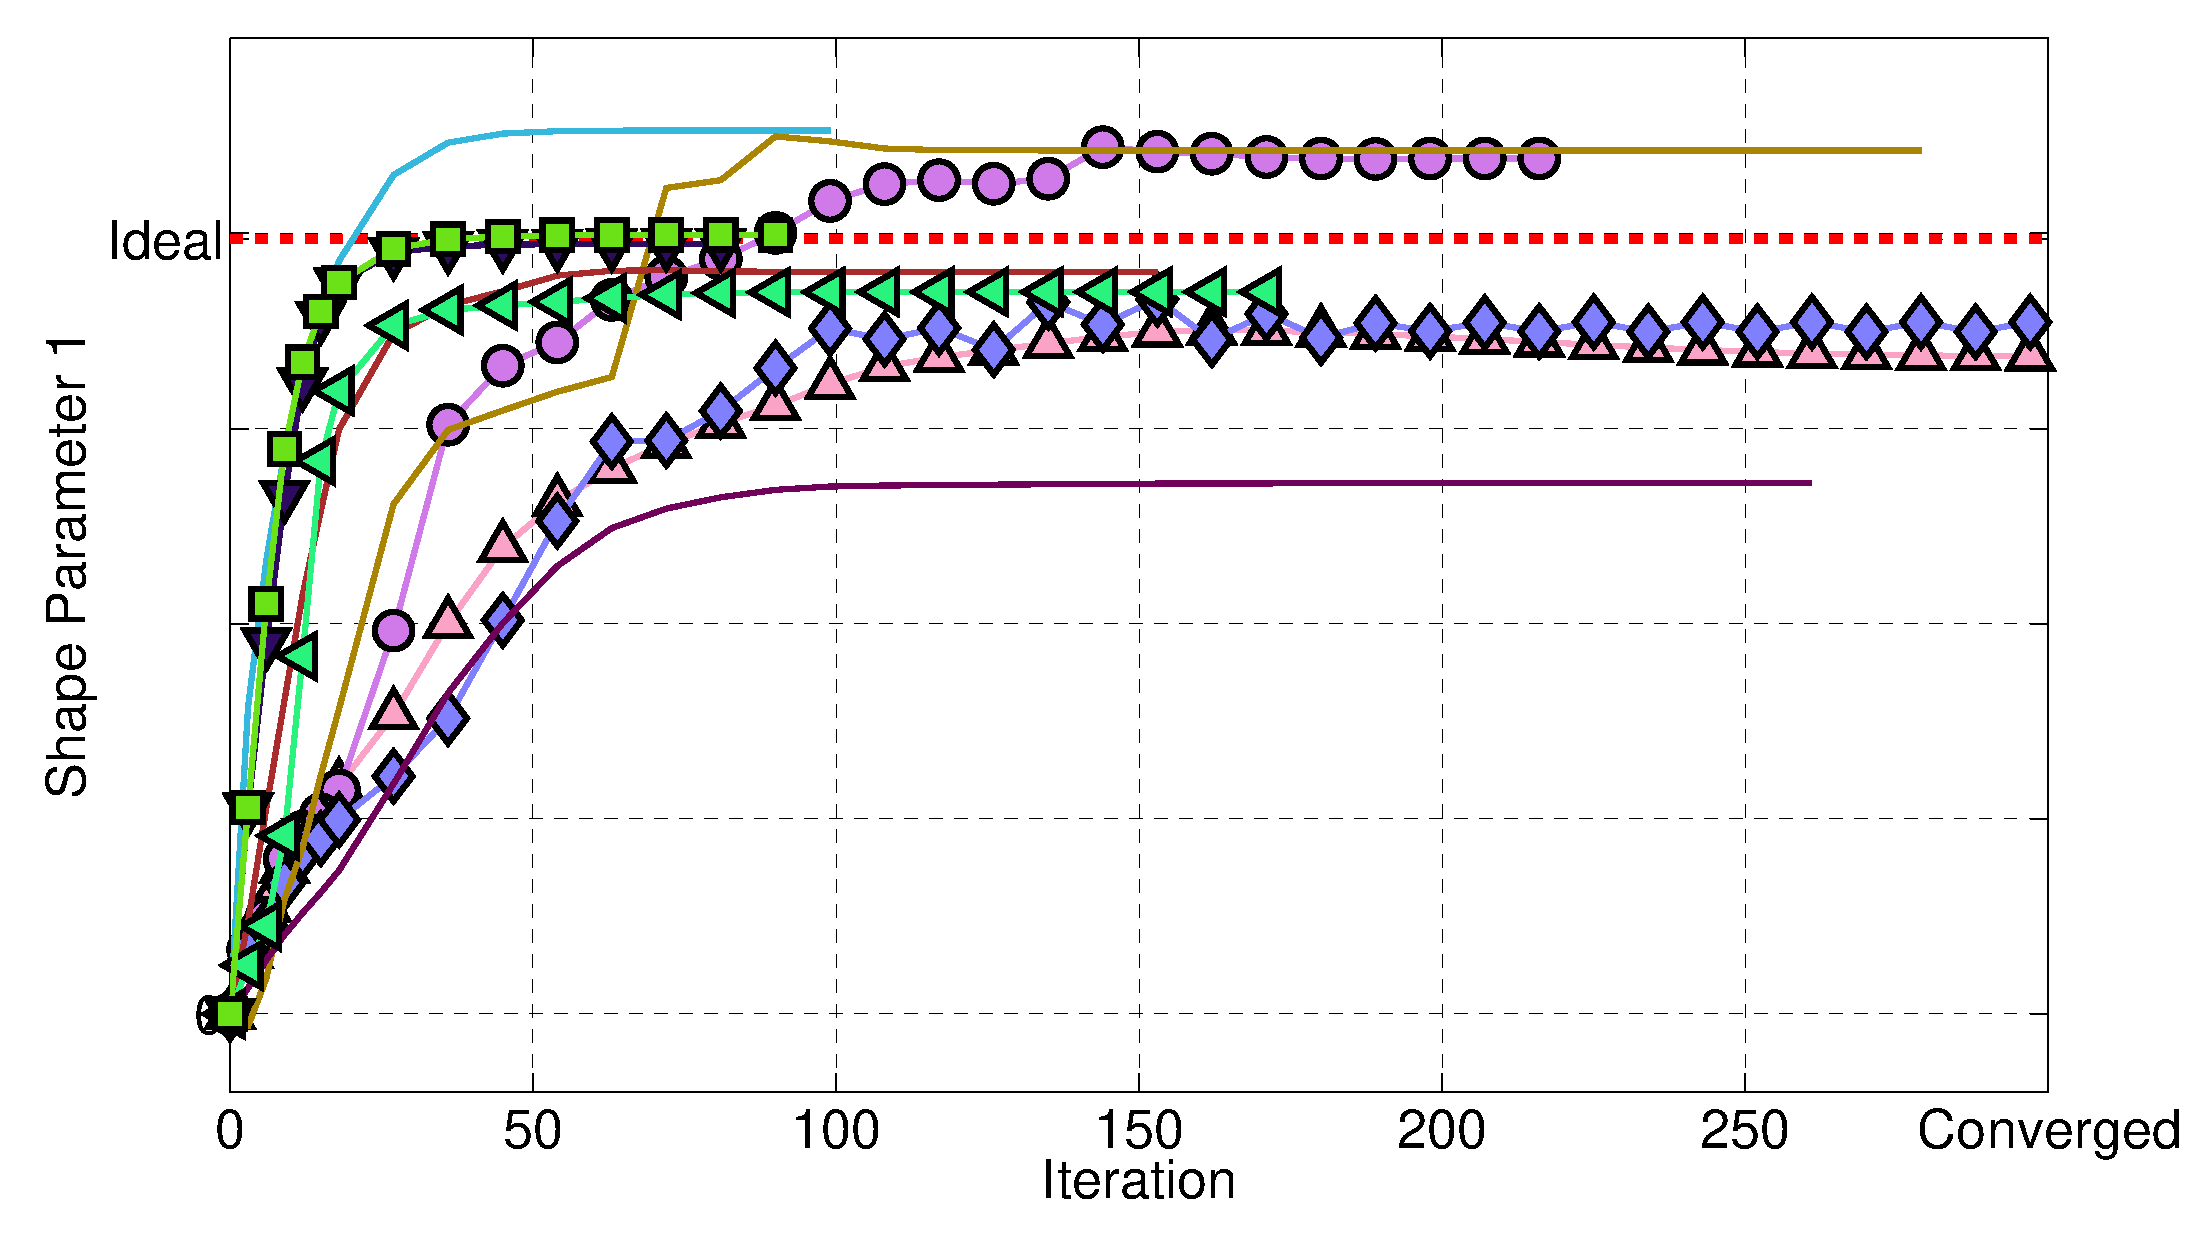
\includegraphics[width=0.70\linewidth]{figures/feature_based_aam/8_AAMconvergenceSpeed/LFPWtest_im22}\\
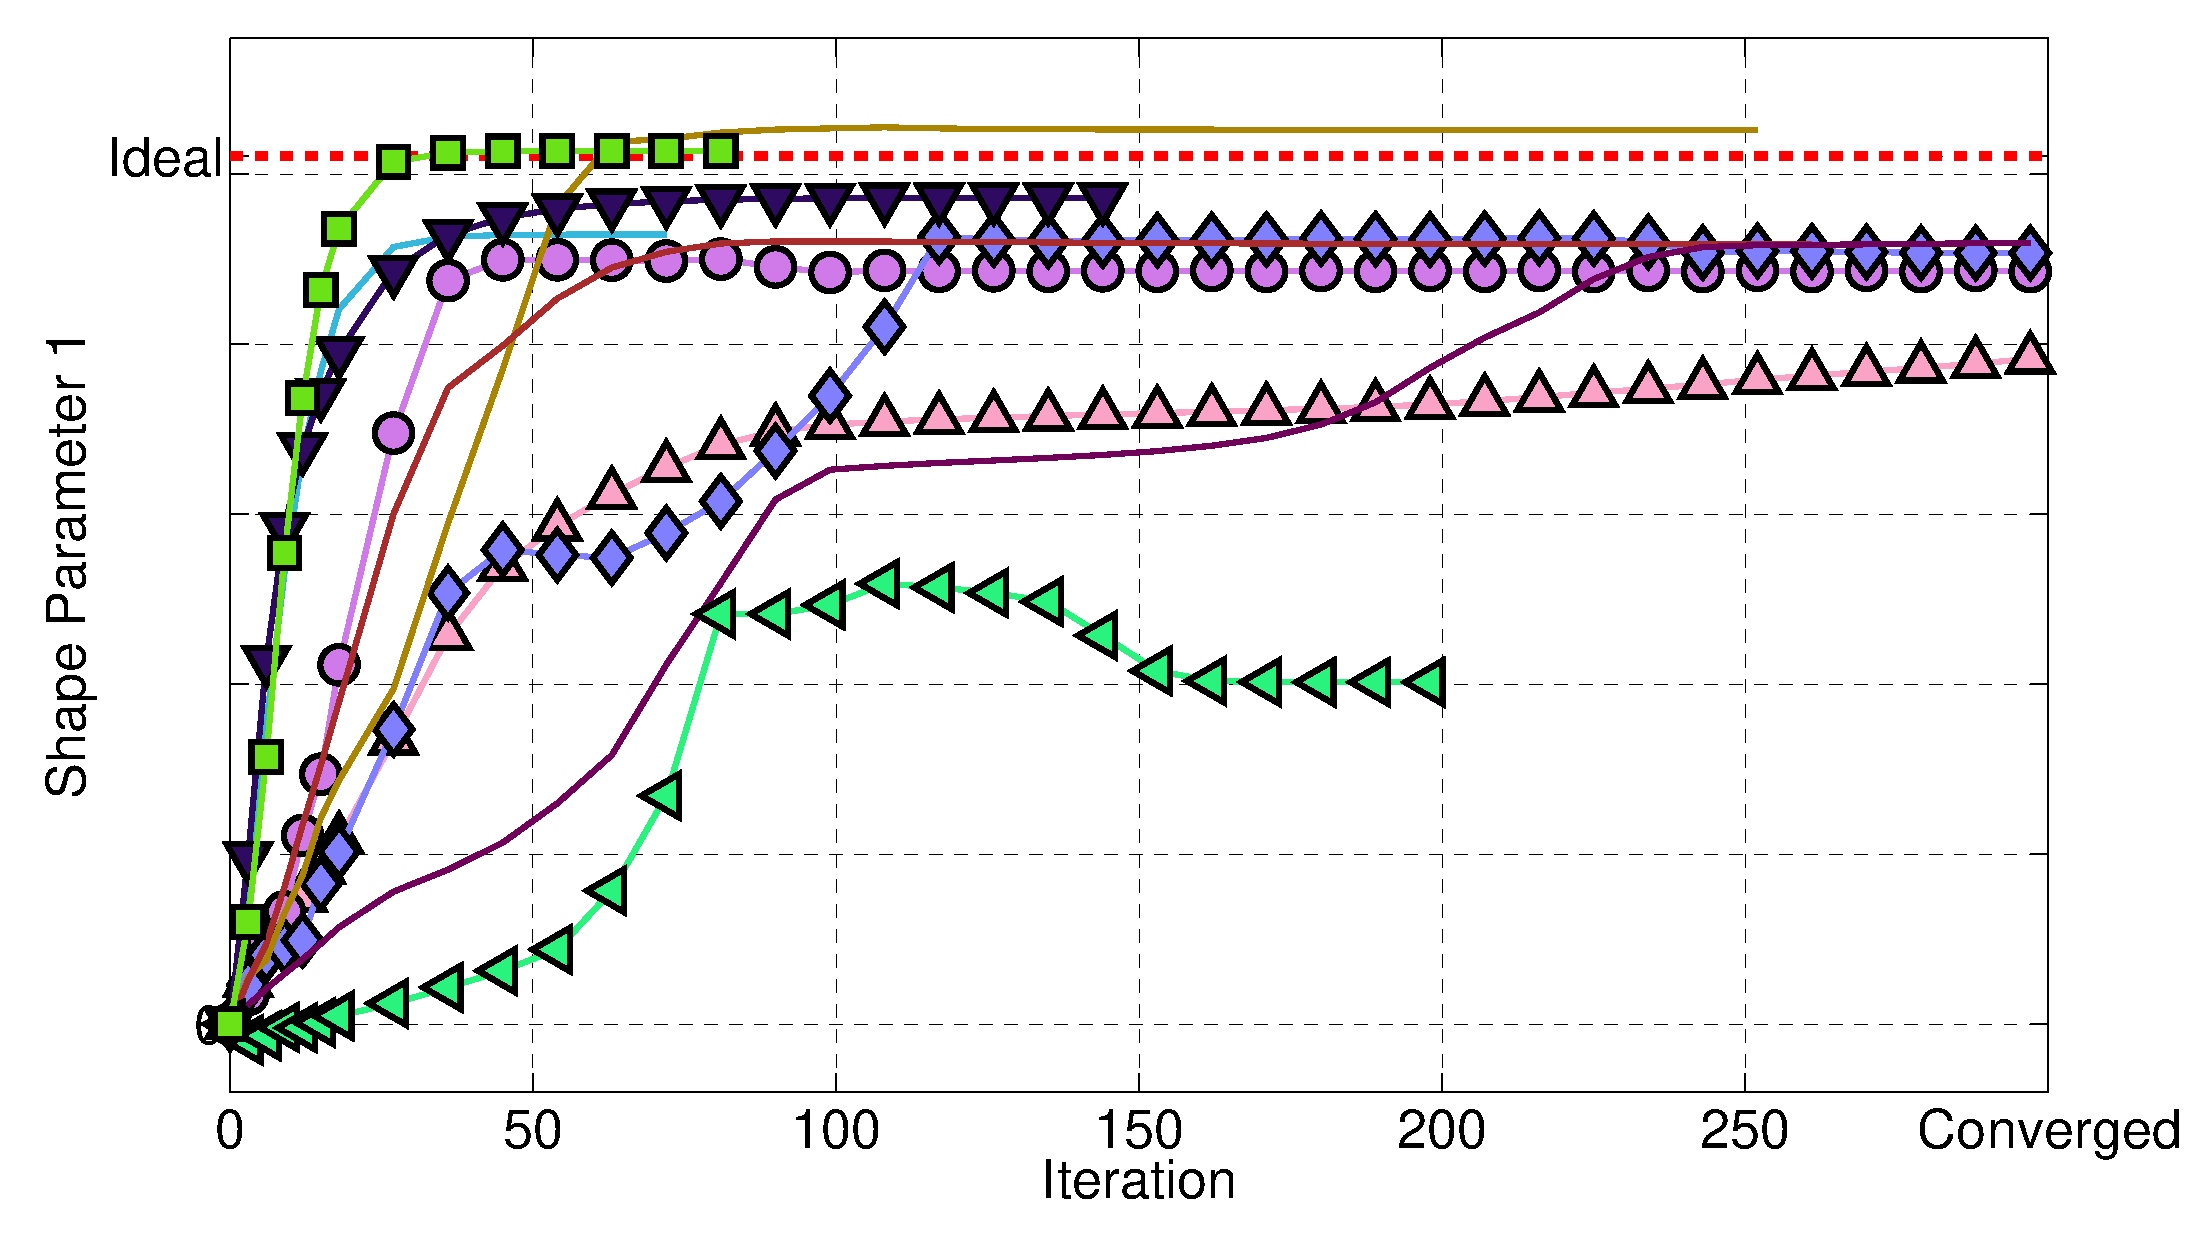
\includegraphics[width=0.70\linewidth]{figures/feature_based_aam/8_AAMconvergenceSpeed/LFPWtest_im28}
\caption{Indicative examples of the speed of convergence of each feature.
The plots show how fast the 1st parameter value of the shape model moves towards
its ideal (groundtruth) value. The example images are \texttt{image\_0022.png}
(\textit{left}) and \texttt{image\_0028.png} (\textit{right}) from LFPW testing set.}
\label{fig:parameterExample}
\end{figure}
%

Figure~\ref{fig:feature_aam:convergence} shows the mean
point-to-point normalized RMS fitting error overall 3026 images with respect to
the iteration number by allowing the optimization procedure to converge. The
results indicate that HOG and SIFT features converge faster to a more accurate
optimum compared to all the other feature types. Indicative examples of the
convergence speed of each feature are shown in Fig.~\ref{fig:parameterExample}.
Specifically, these plots show how fast the parameter value that corresponds to
the 1$^{\text{st}}$ eigenvector of the shape subspace $\mathbf{U}_s$ moves
towards its ideal (ground-truth) value. This eigenshape controls the face's pose
over the yaw angle. These examples demonstrate the advantages of HOG and SIFT
features, which reach the ideal value in very few iterations. Note that in all
these experiments we want the algorithms to converge, thus we let them execute
many iterations. However, this is not necessary in a practical application,
because as the iterations advance, the improvements in the fitted shape get
much smaller.


% Timings table
\begin{table}[!t]
\renewcommand{\arraystretch}{1.3}
\centering
\begin{tabular}{r|c||c|c||c|c|c|c|c|c}
\multicolumn{4}{c||}{} & \multicolumn{6}{c}{\textbf{\emph{Warping on features image}}}\\
\cline{5-10}
& \multirow{3}{*}{\emph{Channels}} & \emph{Feature} & \emph{Warp} & \multicolumn{3}{c|}{\emph{Alternating IC}} & \multicolumn{3}{c}{\emph{Project-Out IC}}\\
\cline{5-10}
\emph{Feature} & & \emph{function} & \emph{function} & \multicolumn{3}{c|}{\emph{number of iterations}} & \multicolumn{3}{c}{\emph{number of iterations}}\\
\emph{Type} & & \emph{Cost ($\mathcal{F}$)} & \emph{Cost ($\mathcal{W}$)} & \emph{1} & \emph{50} & \emph{100} & \emph{1} & \emph{50} & \emph{100}\\ \hline\hline
%
Intensities & 1                   & $-$  & 0.01                  & 0.02 & 1.0  & 2.0  & 0.02 & 1.0  & 2.0\\ \hline
IGO, ES     & 2                   & 0.01 & 0.01                  & 0.05 & 2.0  & 4.0  & 0.04 & 1.5  & 3.0\\ \hline
OLBP        & 8                   & 0.07 & 0.03                  & 0.2  & 6.6  & 13.1 & 0.17 & 5.1  & 10.1\\ \hline
TPLBP       & \multirow{2}{*}{16} & 1.25 & \multirow{2}{*}{0.05} & 1.48 & 12.8 & 24.3 & 1.43 & 10.3 & 19.3\\ \cline{1-1}\cline{3-3}\cline{5-10}
FPLBP       &                     & 1.82 &                       & 2.05 & 13.3 & 24.8 & 2.0  & 10.8 & 19.8\\ \hline
HOG         & \multirow{3}{*}{36} & 1.32 & \multirow{3}{*}{0.11} & 1.84 & 27.3 & 53.3 & 1.72 & 21.3 & 41.3\\ \cline{1-1}\cline{3-3}\cline{5-10}
SIFT        &                     & 0.07 &                       & 0.59 & 26.1 & 52.1 & 0.47 & 20.1 & 40.1\\ \cline{1-1}\cline{3-3}\cline{5-10}
Gabor       &                     & 0.12 &                       & 0.64 & 26.1 & 52.1 & 0.52 & 20.1 & 40.1\\
\hline\hline\hline
\multicolumn{4}{c||}{} & \multicolumn{6}{c}{\textbf{\emph{Features from warped image}}}\\
\cline{5-10}
& \multirow{3}{*}{\emph{Channels}} & \emph{Feature} & \emph{Warp} & \multicolumn{3}{c|}{\emph{Alternating IC}} & \multicolumn{3}{c}{\emph{Project-Out IC}}\\
\cline{5-10}
\emph{Feature} & & \emph{function} & \emph{function} & \multicolumn{3}{c|}{\emph{number of iterations}} & \multicolumn{3}{c}{\emph{number of iterations}}\\
\emph{Type} & & \emph{Cost ($\mathcal{F}$)} & \emph{Cost ($\mathcal{W}$)} & \emph{1} & \emph{50} & \emph{100} & \emph{1} & \emph{50} & \emph{100}\\
\hline\hline
%
Intensities & 1                   & $-$  & 0.01                  & 0.02 & 1.0   & 2.0   & 0.02 & 1.0  & 2.0   \\ \hline
IGO, ES     & 2                   & 0.01 & 0.01                  & 0.04 & 2.0   & 4.0   & 0.03 & 1.5  & 3.0   \\ \hline
OLBP        & 8                   & 0.07 & 0.03                  & 0.18 & 9.0   & 18.0  & 0.15 & 7.5  & 15.0  \\ \hline
TPLBP       & \multirow{2}{*}{16} & 1.25 & \multirow{2}{*}{0.05} & 1.44 & 72.0  & 144.0 & 1.39 & 69.5 & 139.0 \\ \cline{1-1}\cline{3-3}\cline{5-10}
FPLBP       &                     & 1.82 &                       & 2.01 & 100.5 & 201.0 & 1.96 & 98.0 & 196.0 \\ \hline
HOG         & \multirow{3}{*}{36} & 1.32 & \multirow{3}{*}{0.11} & 1.74 & 87.7  & 174.0 & 1.62 & 81.0 & 162.0 \\ \cline{1-1}\cline{3-3}\cline{5-10}
SIFT        &                     & 0.07 &                       & 0.49 & 24.5  & 49.0  & 0.37 & 18.5 & 37.0  \\ \cline{1-1}\cline{3-3}\cline{5-10}
Gabor       &                     & 0.12 &                       & 0.54 & 27.0  & 54.0  & 0.42 & 21.0 & 42.0
%
\end{tabular}
\caption{Computational costs of the feature extraction functions, the warp function and the AAM fitting using both composition ways of the two functions for all feature types. All the reported times are measured in seconds.}
\label{tab:times}
\end{table}
%

% Timings
\subsubsection{Timings}\label{sec:aam:timings}
Table~\ref{tab:times} reports the timings for each feature type using the two
compositional scenarios explained in Sec.~\ref{sec:aam:featureBasedOptimization}
within the AAMs optimization framework. It presents the computational cost per
iteration and the total cost of running the optimization for 50 and 100 iterations.
Note that the AAMs framework used for those experiments is developed without any
code optimization. The reference frame (mean shape $\bar{\mathbf{s}}$) has size
$170\times170$.

The table justifies the computational analysis presented in
Sec.~\ref{sec:aam:featureBasedOptimization}. As expected, it is faster to compute
the features once and warp the features image (Eq.~\ref{equ:featuresWarpCost})
rather than extracting features from each warped image at each iteration
(Eq.~\ref{equ:warpFeaturesCost}). This is because, in most features cases,
it is more expensive to extract features than warp a multi-channel image
($\mathcal{O}(\mathcal{F})>\mathcal{O}(\mathcal{W})$). This happens with all
the multi-channel features. The only exception is the SIFT features case,
because the optimized implementation of~\cite{vedaldi2008vlfeat} is faster
than the unoptimized warping of the 36 channels
($\mathcal{O}(\mathcal{F})<\mathcal{O}(\mathcal{W})$). Moreover, the combination
of Tab.~\ref{tab:times} with Fig.~\ref{fig:feature_aam:convergence} suggests
that even though high-dimensional features like HOG and SIFT converge really
fast, their computational cost is quite similar to features with less channels
that require multiple iterations until convergence.

The AAM fitting used in these experiments is implemented in
Matlab using the Moore-Penrose pseudoinverse, which, despite the fact that it
ensures robustness, it is computationally expensive. Additionally, as mentioned
before, the fitting is not performed using an image pyramid. These two factors
make the fitting procedure reported in Tab.~\ref{tab:times} slower than expected.
However, note that the aim of these experiments is to make a fair comparison of
the computational complexity between the different feature types. It is not in the
scope of this work to provide an optimized implementation of AAMs or features.
Faster AAM optimization can be achieved with the framework proposed
in~\cite{papandreou2008adaptive,tzimiropoulos2013optimization}. One could also use GPU or parallel
programming to achieve faster performance and eliminate the cost difference
between various features and also between the two composition scenarios of
$\mathcal{F}$ and $\mathcal{W}$. Finally, by applying a multi-scale fitting using
an image pyramid greatly speeds up the fitting procedure, since convergence is
achieved in less iterations, as shown in Chapter~\ref{ch:aps} (Sec.~\ref{sec:aps:exp})
and Chapter~\ref{ch:acr}.

% Number of Appearance Components
\begin{figure}[!h]
\centering
\hspace{0.65cm}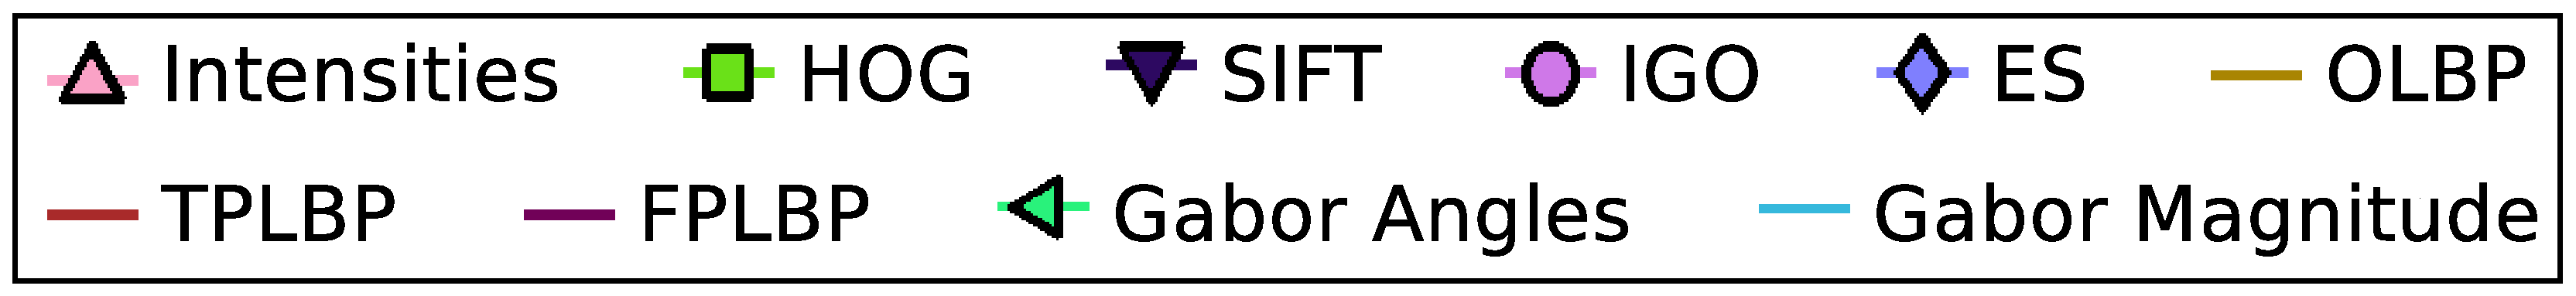
\includegraphics[height=0.90cm]{figures/feature_based_aam/9_AAMnumberOfAppearanceComponents/legend}\\
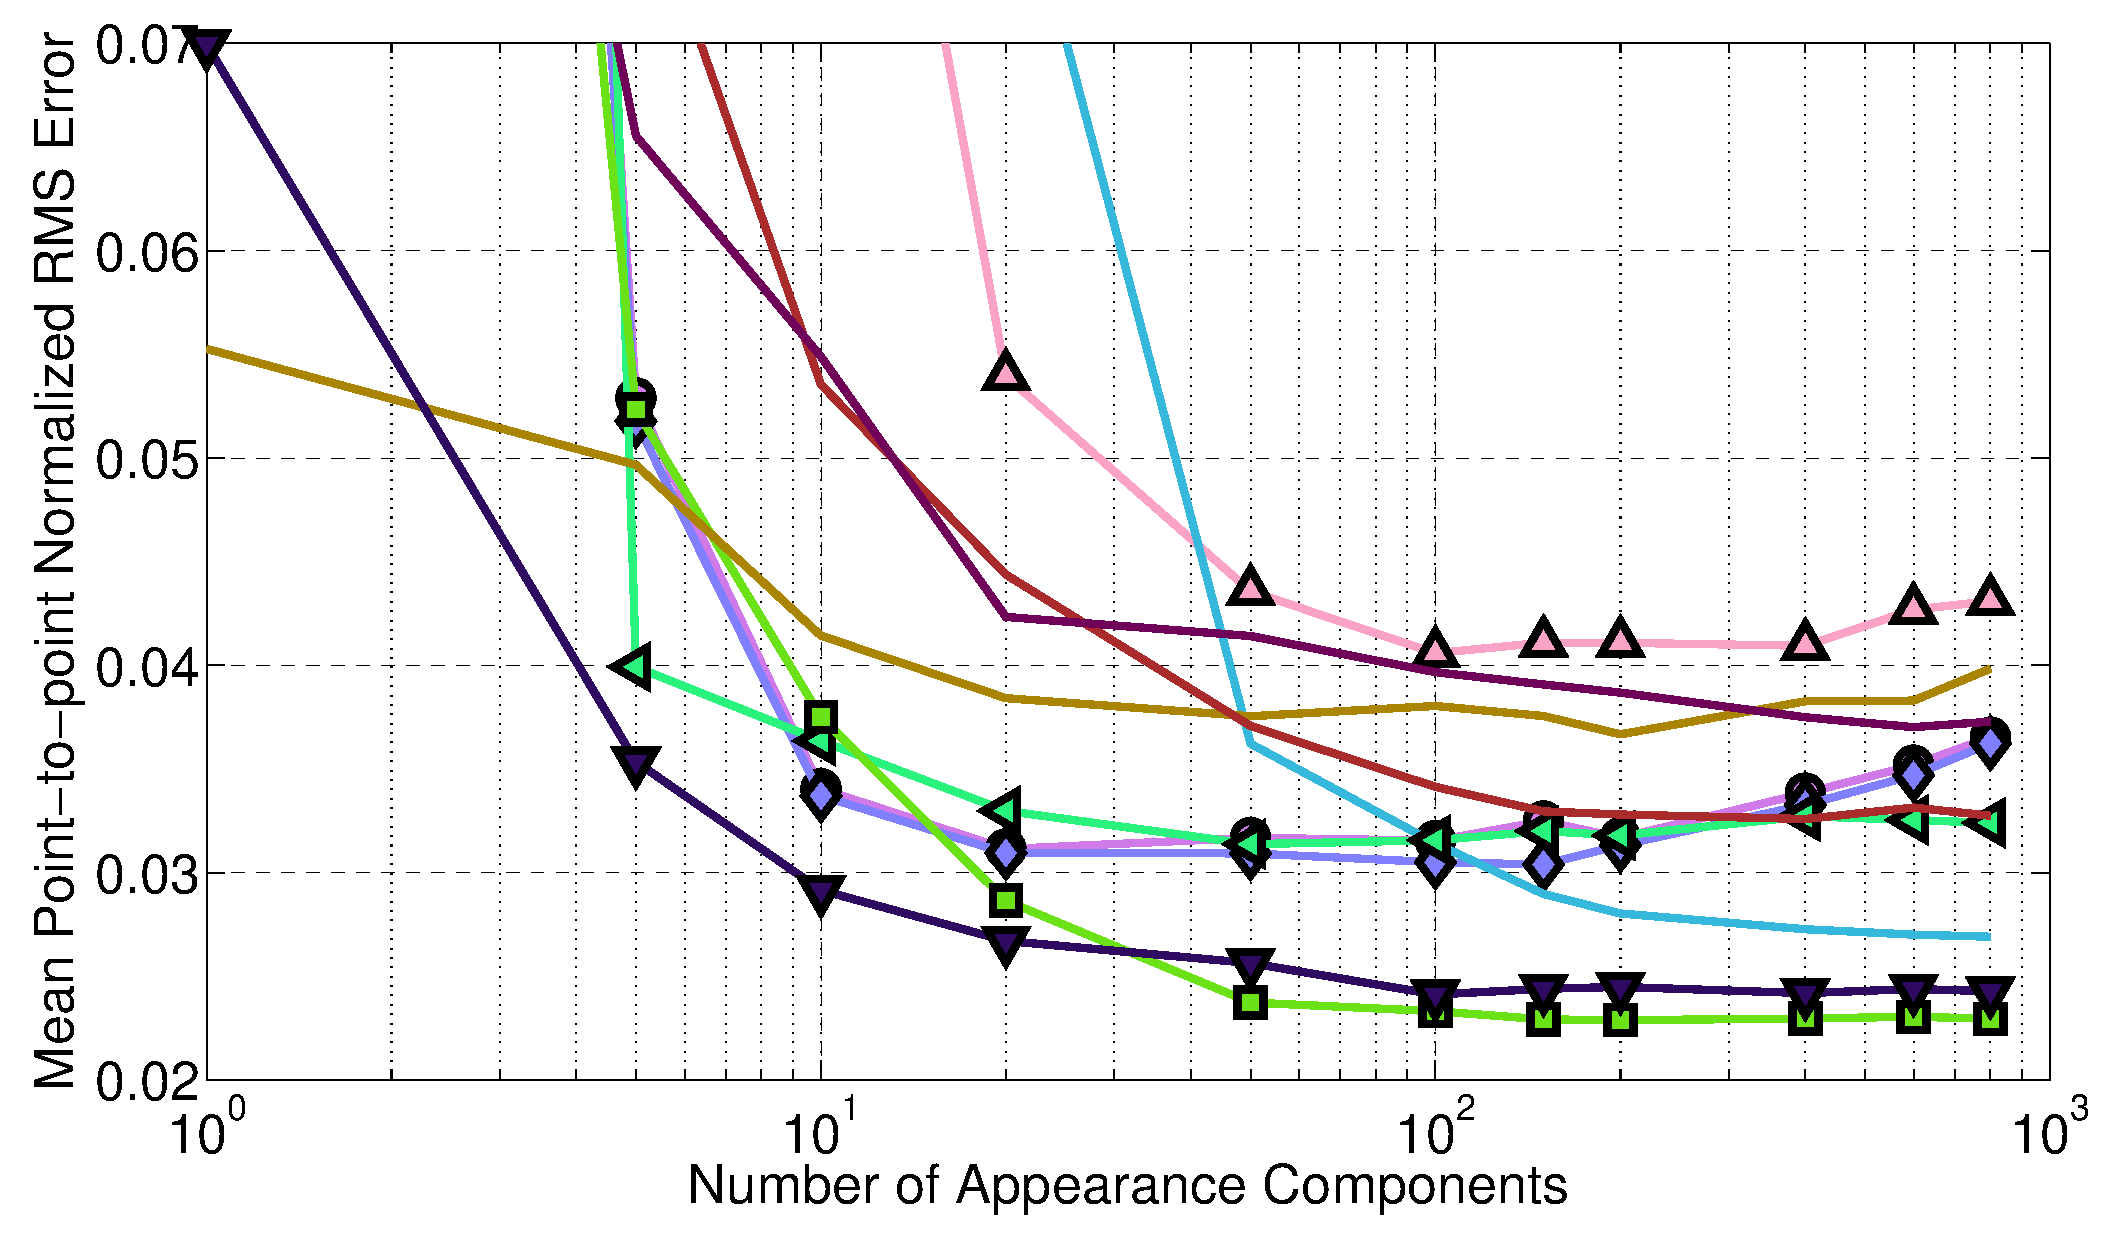
\includegraphics[width=0.70\linewidth]{figures/feature_based_aam/9_AAMnumberOfAppearanceComponents/experiment}
\caption{Mean point-to-point normalized RMS fitting error with respect to number
of appearance components on the LFPW testset in-the-wild database.
Note that we use logarithmic scale on the horizontal axis.}
\label{fig:n_components}
\end{figure}
%

% Number of Appearance Components
\subsubsection{Number of Appearance Components}\label{sec:aam:n_components}
Figure~\ref{fig:n_components} shows the mean point-to-point normalized RMS
fitting error with respect to the number of appearance components, i.e. $n_a$,
for LFPW testset using logarithmic scale on the horizontal axis. The results
indicate that for most features, except IGO, ES and Intensities, the fitting
performance is improved by increasing the number of appearance components. SIFT
features can achieve very accurate results by using very few appearance components
(even less than 10), thus with small computational cost. Additionally, note that
Gabor Magnitude features can achieve significantly good accuracy (close to HOG and SIFT)
if one keeps their whole eigenspectrum.

% Neighbourhood Size
\begin{figure}[!h]
\centering
\hspace{0.5cm}\includegraphics[height=0.90cm]{figures/feature_based_aam/10_AAMneighbourhoodSize/legend}\\
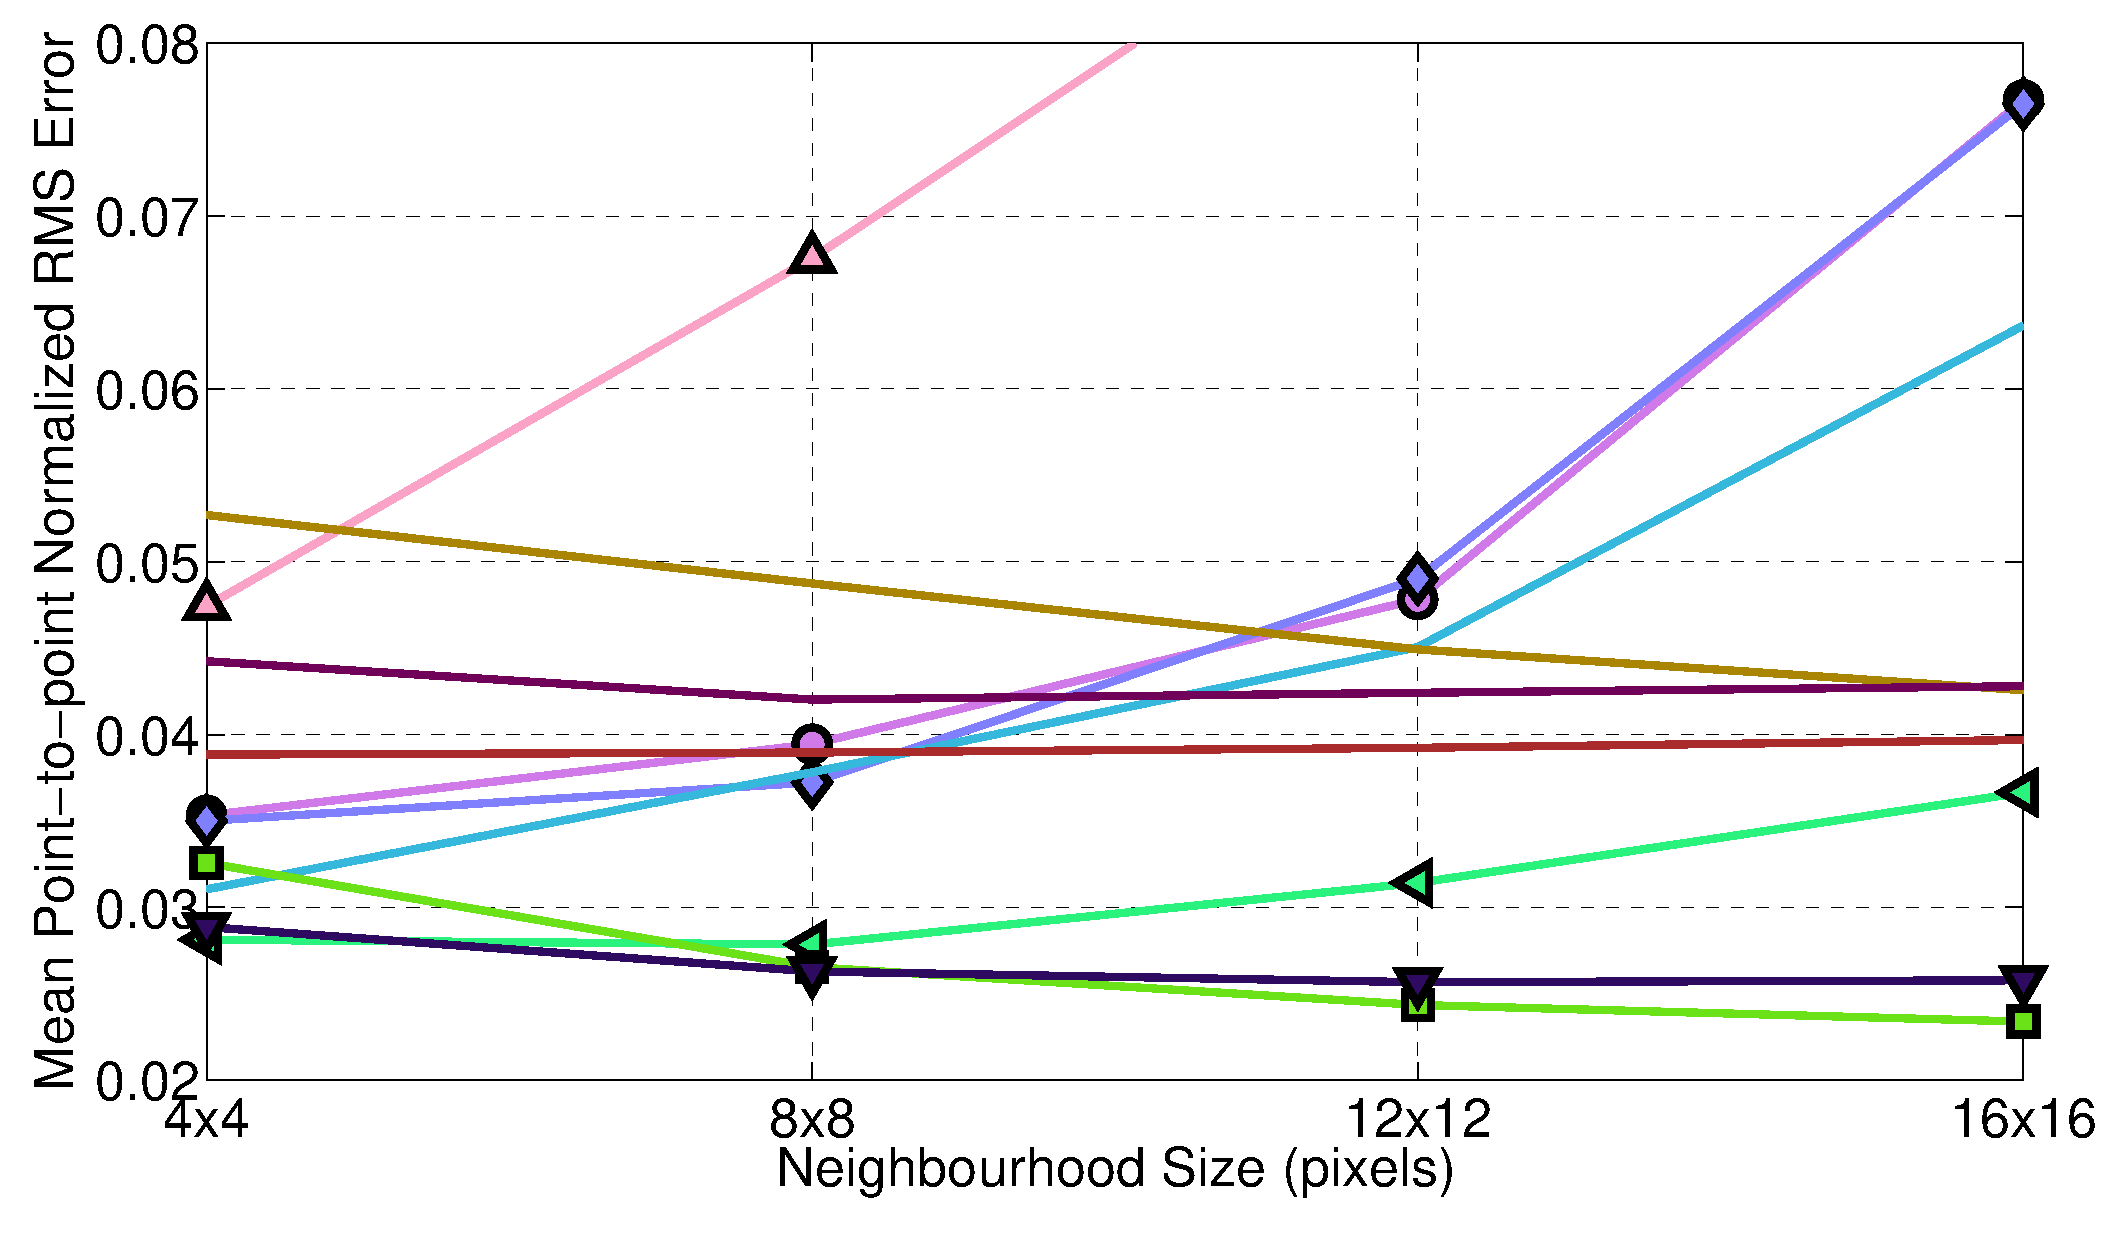
\includegraphics[width=0.70\textwidth]{figures/feature_based_aam/10_AAMneighbourhoodSize/experiment}
\caption{Mean point-to-point normalized RMS fitting error with respect to
neighbourhood size on the LFPW testset in-the-wild database.}
\label{fig:neighbourhood_size}
\end{figure}
%

% Neighbourhood Size
\subsubsection{Neighborhood Size}\label{sec:aam:neighbourhood}
Figure~\ref{fig:neighbourhood_size} plots the mean point-to-point normalized
RMS fitting error with respect to the neighborhood size from which the feature
value of each pixel is computed. For HOG and SIFT this is done by changing the
cell size. In the case of the LBPs family, we alter the radius values ($N_{radius}$).
For the rest of features (IGO, ES, Gabor, Intensities), we simply downscale the image.
This experiment proves that the spatial neighborhood covered by each feature
does not massively affect its performance. HOG, SIFT and LBP features are more
accurate when applied to largest regions, as more information is accumulated to
their channels. On the contrary, ES, IGO and Gabor features are not assisted
by increasing the neighborhood size.

% Contour plots
\begin{figure}[!h]
\centering
\includegraphics[height=0.3cm]{figures/feature_based_aam/11_CostFunction/colorbar.png}\\
\subfloat[Intensities]{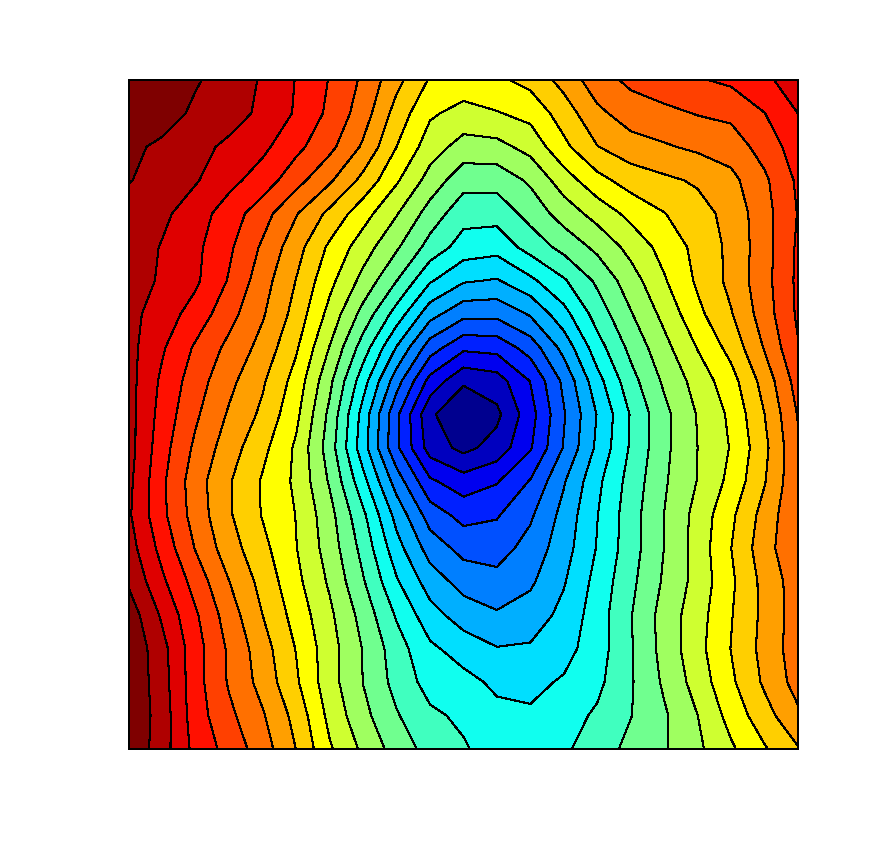
\includegraphics[width=0.2\linewidth]{figures/feature_based_aam/11_CostFunction/intensities}\label{fig_cost:intensities}}
\hfil
\subfloat[ES]{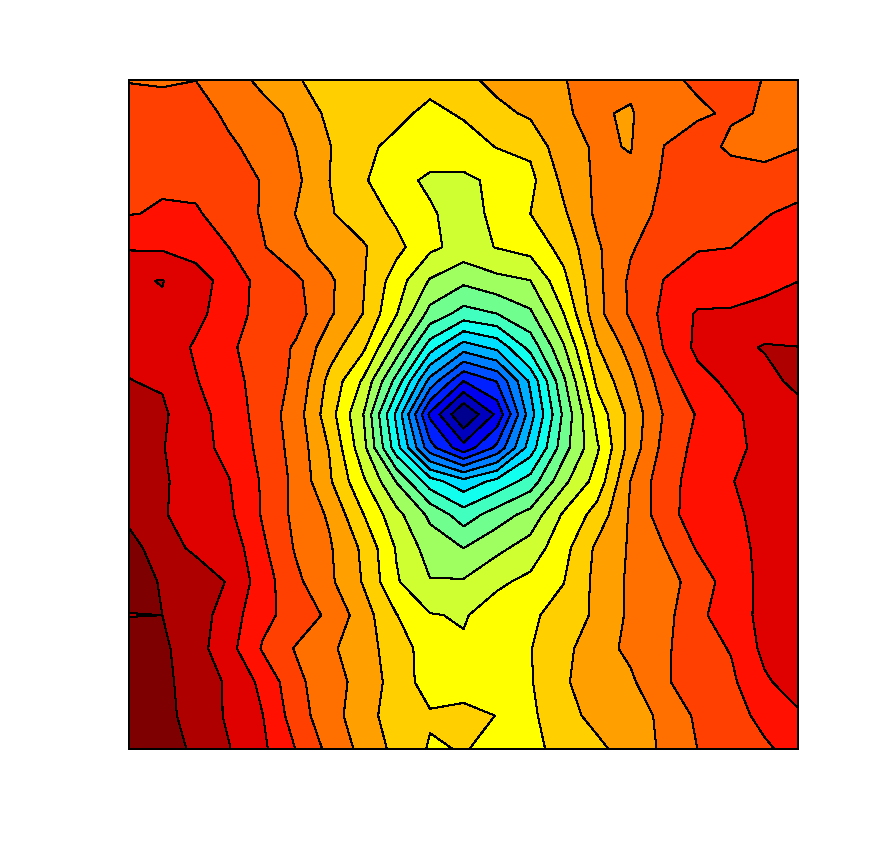
\includegraphics[width=0.2\linewidth]{figures/feature_based_aam/11_CostFunction/es}\label{fig_cost:es}}
\hfil
\subfloat[IGO]{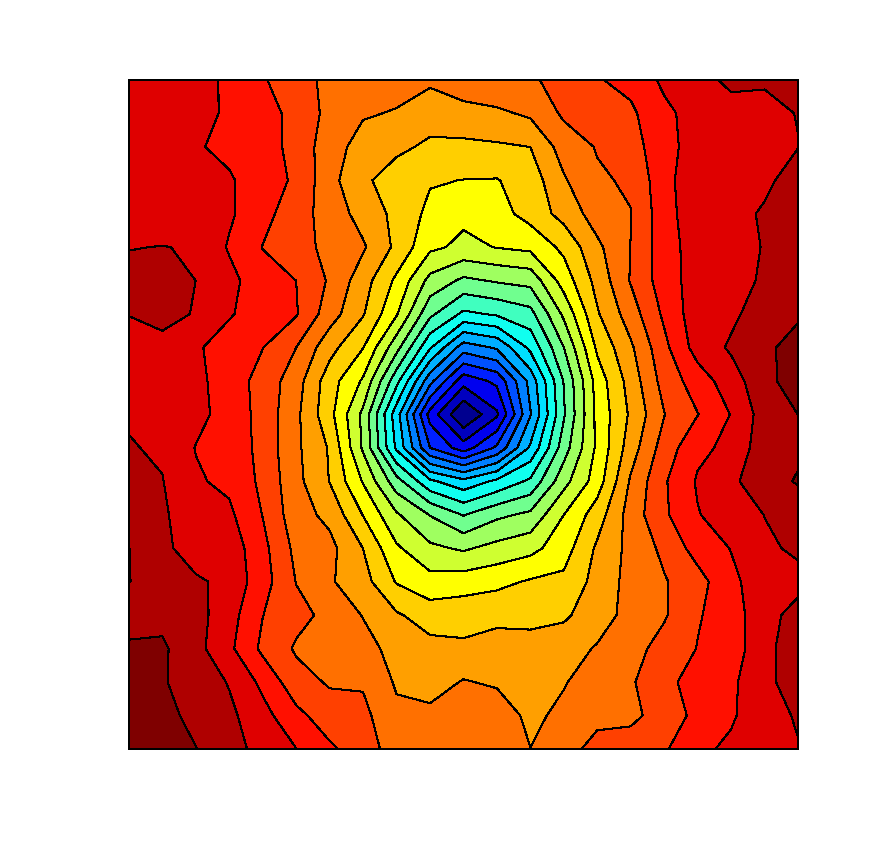
\includegraphics[width=0.2\linewidth]{figures/feature_based_aam/11_CostFunction/igo}\label{fig_cost:igo}}
\hfil
\subfloat[HOG]{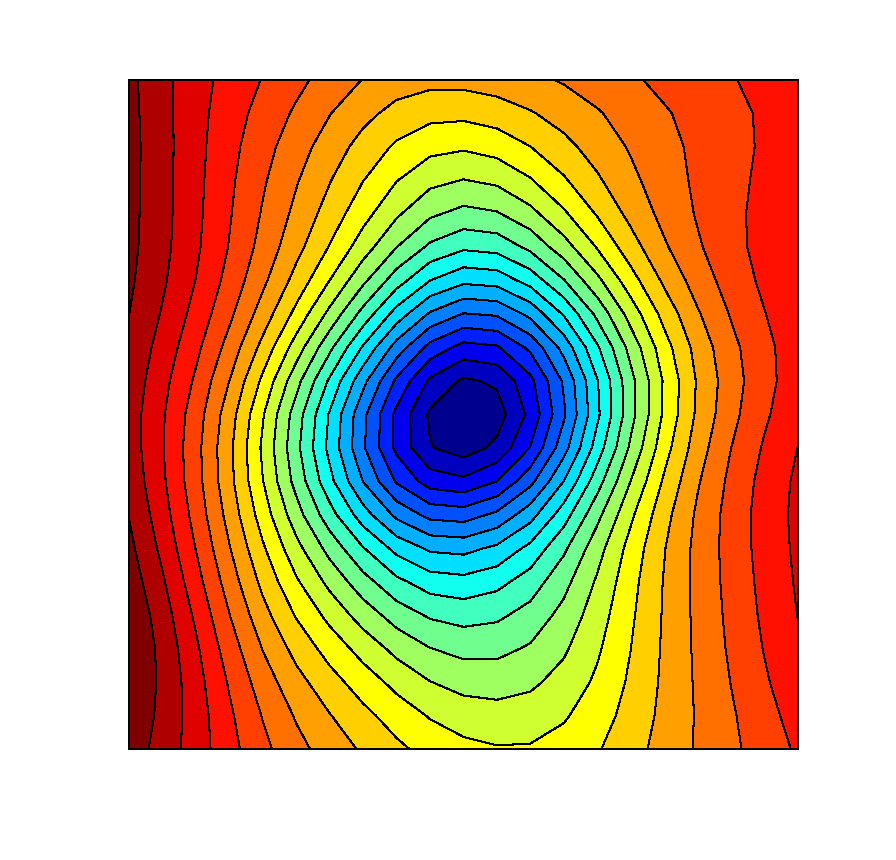
\includegraphics[width=0.2\linewidth]{figures/feature_based_aam/11_CostFunction/hog}\label{fig_cost:hog}}
\hfil
\subfloat[SIFT]{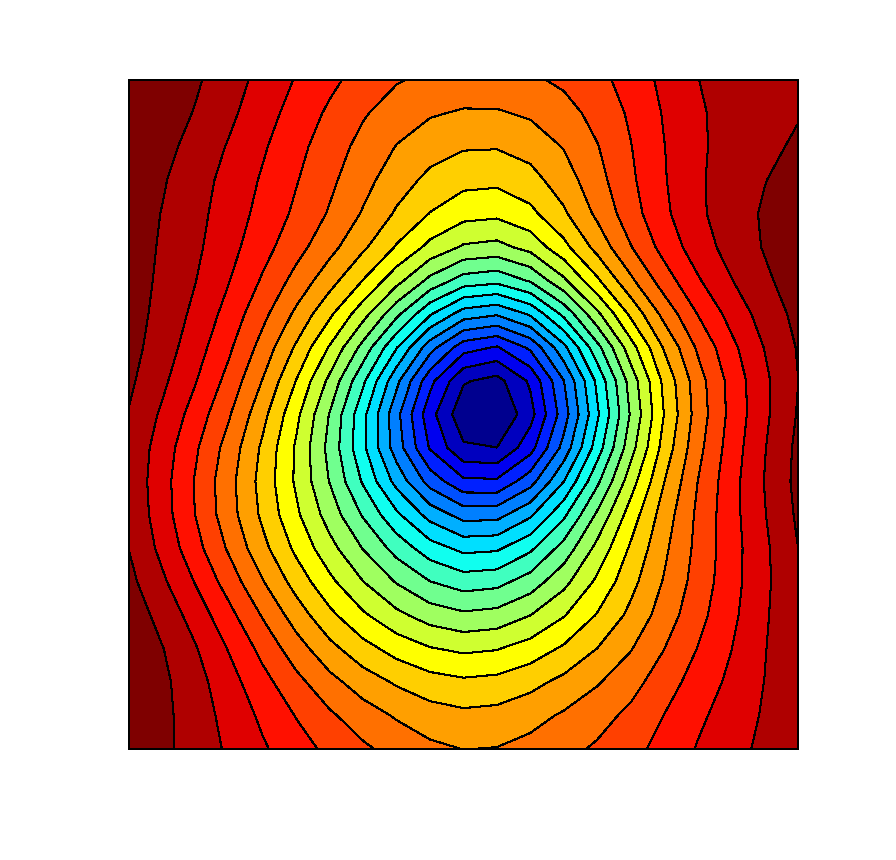
\includegraphics[width=0.2\linewidth]{figures/feature_based_aam/11_CostFunction/sift}\label{fig_cost:sift}}\\
\subfloat[OLBP]{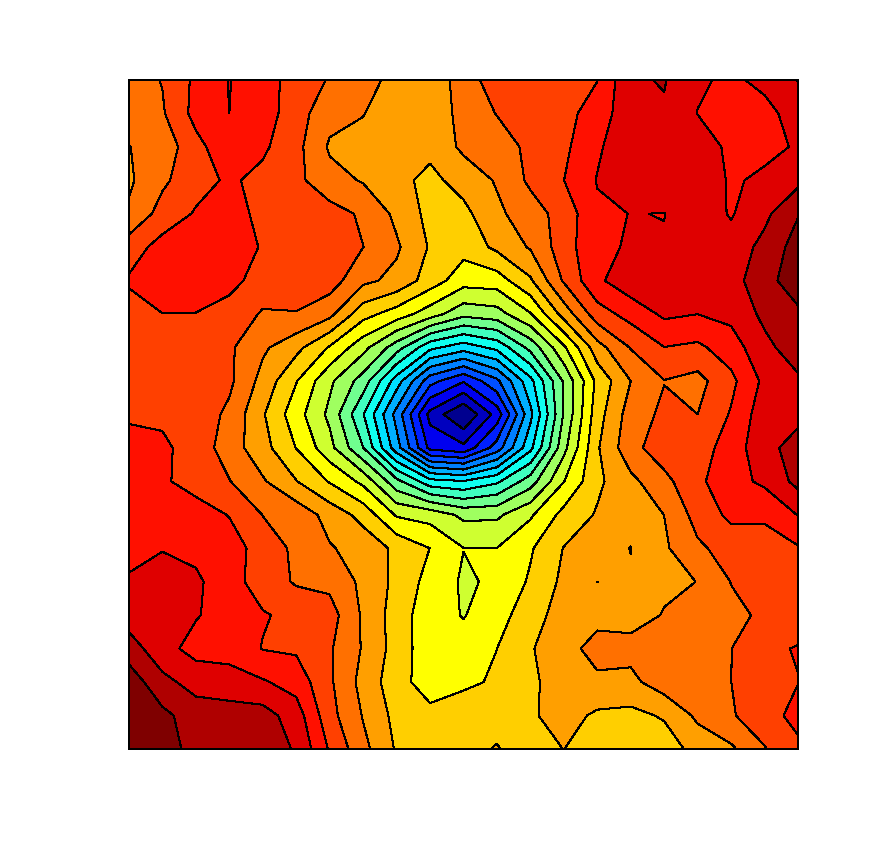
\includegraphics[width=0.2\linewidth]{figures/feature_based_aam/11_CostFunction/lbp}\label{fig_cost:olbp}}
\hfil
\subfloat[TPLBP]{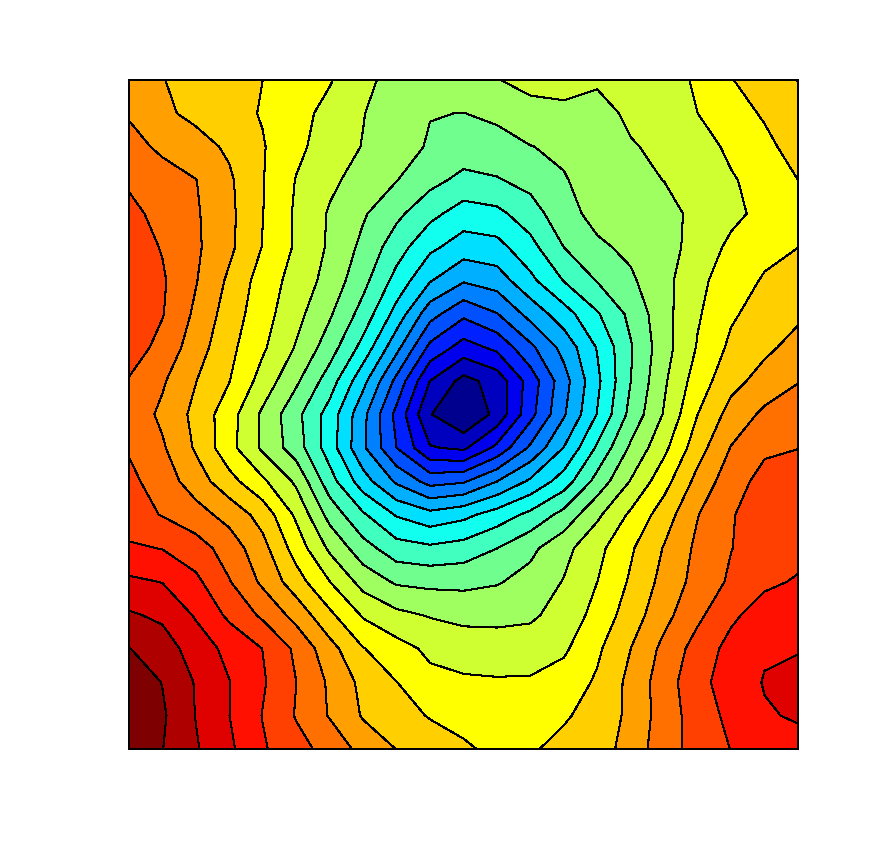
\includegraphics[width=0.2\linewidth]{figures/feature_based_aam/11_CostFunction/tplbp}\label{fig_cost:tplbp}}
\hfil
\subfloat[FPLBP]{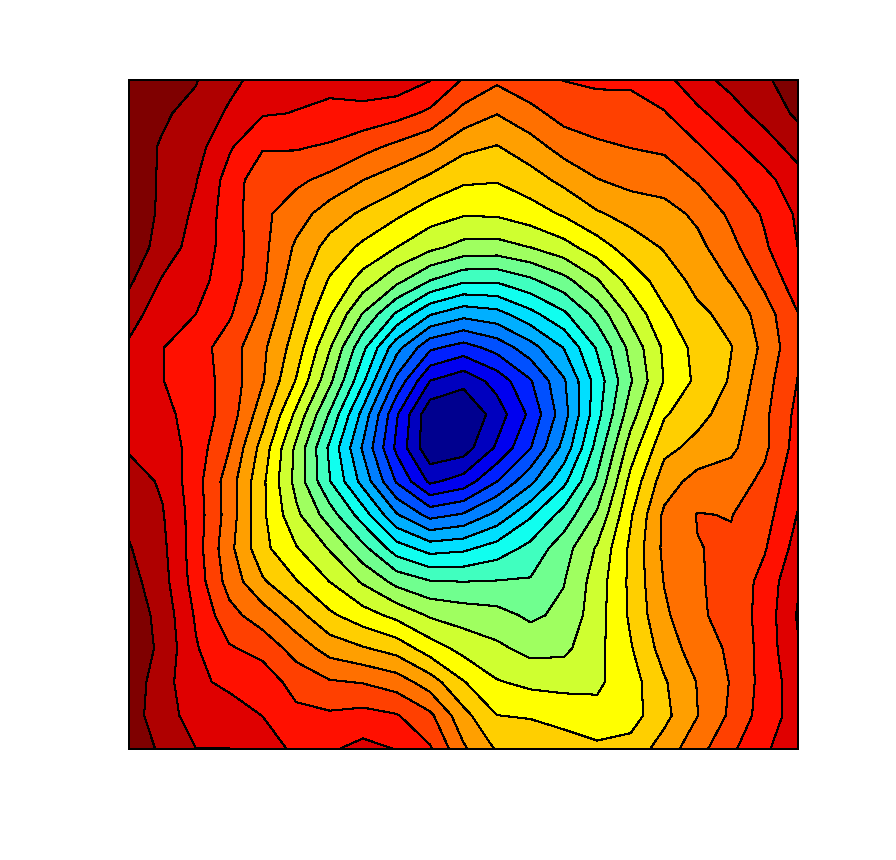
\includegraphics[width=0.2\linewidth]{figures/feature_based_aam/11_CostFunction/fplbp}\label{fig_cost:fplbp}}
\hfil
\subfloat[Gabor Angles]{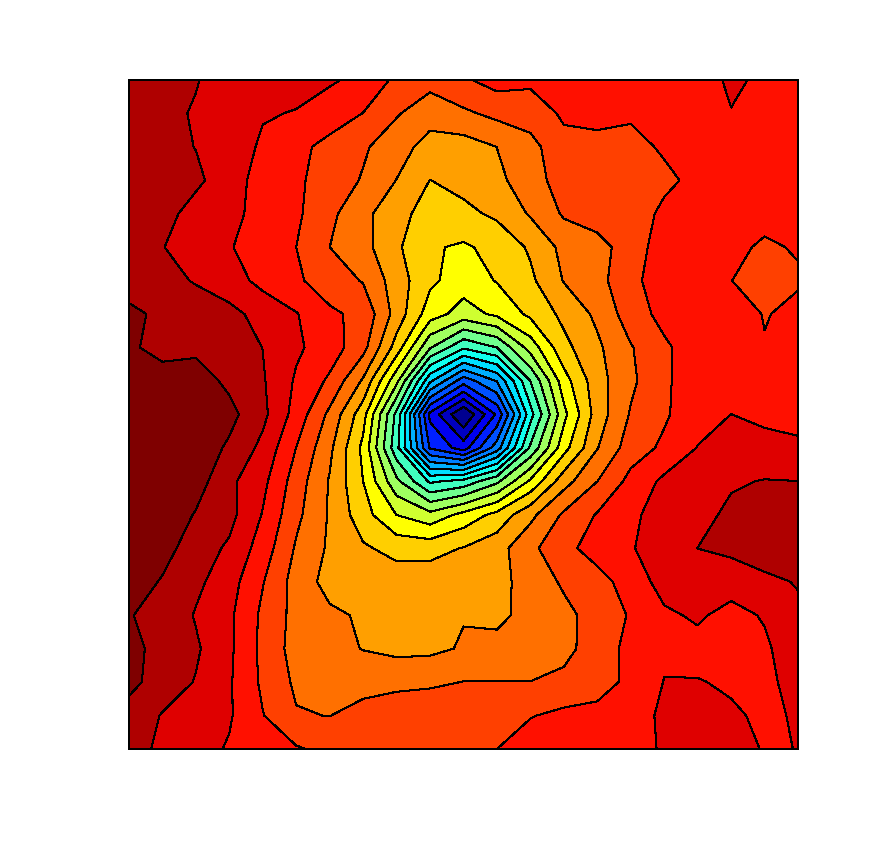
\includegraphics[width=0.2\linewidth]{figures/feature_based_aam/11_CostFunction/gabor_angles}\label{fig_cost:gabor_angles}}
\hfil
\subfloat[Gabor Magnitude]{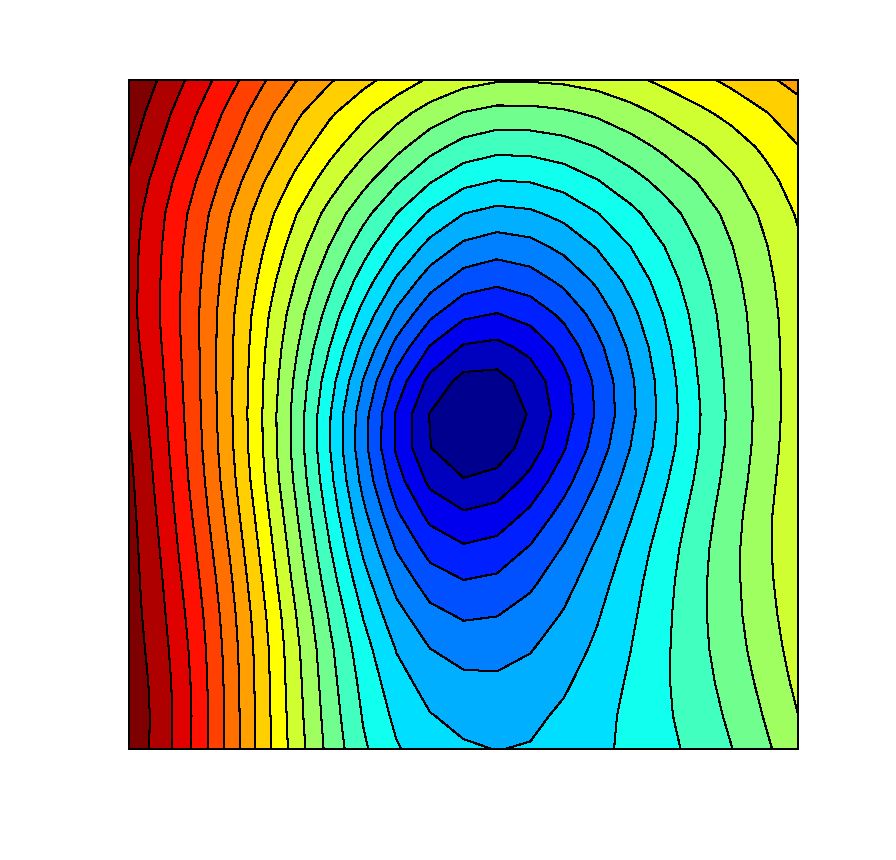
\includegraphics[width=0.2\linewidth]{figures/feature_based_aam/11_CostFunction/gabor_magnitude}\label{fig_cost:gabor_magnitude}}
\caption{Contour plots of the cost function for each feature. The plots show the mean cost function over 100 images after translating the ground-truth shape over the $x$ and $y$ axis by $\pm15\%$ (pixels) of the face size.}
\label{fig:cost_function}
\end{figure}
%

% Cost Function
\subsubsection{Cost Function}\label{sec:aam:cost_function}
Figure~\ref{fig:cost_function} illustrates the cost function for each feature
type in 2D contour plots. The plots are generated by translating the ground-truth
shape of an image within a grid of $\pm15\%$ (pixels) of the face size along
the $x$ and $y$ axis and evaluating the cost of Eq.~\ref{equ:minimizationCostForAAMs},
where $\mathbf{c}$ are the projection parameters
$\mathbf{c} = \mathbf{U}_a^{\mathsf{T}} (\mathbf{t}(\mathcal{W}(\mathbf{p}))-\bar{\mathbf{a}})$.
The plotted costs are averaged over 100 images. For each feature
we use $n_a=100$ appearance components, so that the experiment is fair and can
be combined with the accuracy results of Sec.~\ref{sec:aam:accuracy}.
These plots are very informative. The cost functions of IGO, ES and Gabor Angles
have a very narrow region of small errors, which means that they can be
accurate only when their initialization is close to the global optimum.
On the contrary, Gabor Magnitude features have a very broad low error region,
which means that they can quickly reach a small error but they will get stuck
to a local minimum that is probably far from the global optimum. This can also
be observed in Fig.~\ref{fig:convergence:alternating}, where Gabor Magnitude
features converge very fast to a low error but then start to diverge, due to
the multiple local minima of their cost function. Finally, HOG and SIFT features
have a smooth cost and the region of minimum values is large enough to
facilitate fast and accurate convergence.



% Comparison with state-of-the-art face fitting methods
\subsection{Comparison with state-of-the-art Face Fitting Methods}\label{subsec:aam:comparison}
Herein we compare the performance of our proposed feature-based AAMs
(both AIC and POIC) against two state-of-the-art facial trackers: Supervised
Descent Method (SDM)~\cite{xiong2013supervised} and
Robust Discriminative Response Map Fitting (DRMF) for
Constrained Local Models (CLMs)~\cite{asthana2013robust}.
For our feature-based AAMs, we employ the HOG and SIFT features because they
proved to be the most accurate and robust for both face alignment and fitting.
We use the same initialization and experimental setup as in the previous section
(Sec.~\ref{subsec:aam:AAMs}). Specifically, the AAMs are trained on the 811
images of the LFPW trainset, keeping $n_s=15$ eigenshapes and $n_a=100$
eigentextures.
For the other two methods, we used the implementations provided online by their
authors with their pre-trained models. Note that both these methods are trained
on thousands of images, much more than the 811 used to train our AAMs. All
methods are initialized using the CDPM face
detector~\cite{orozco2013empirical}. In this experiment we
report results evaluated on 49 landmark points shape mask instead of 68 points.
This is because the SDM framework computes and returns only these 49 points.
The 49-point mask occurs by removing the 17 points of the boundary (jaw) and
the 2 points the mouth's corners from the 68 points shape mask
of~\cite{gross2010multi}. Thus this evaluation scheme emphasizes on
the internal facial areas (eyebrows, eyes, nose, mouth).

% Number Of Training Images
\begin{figure}[!h]
\centering
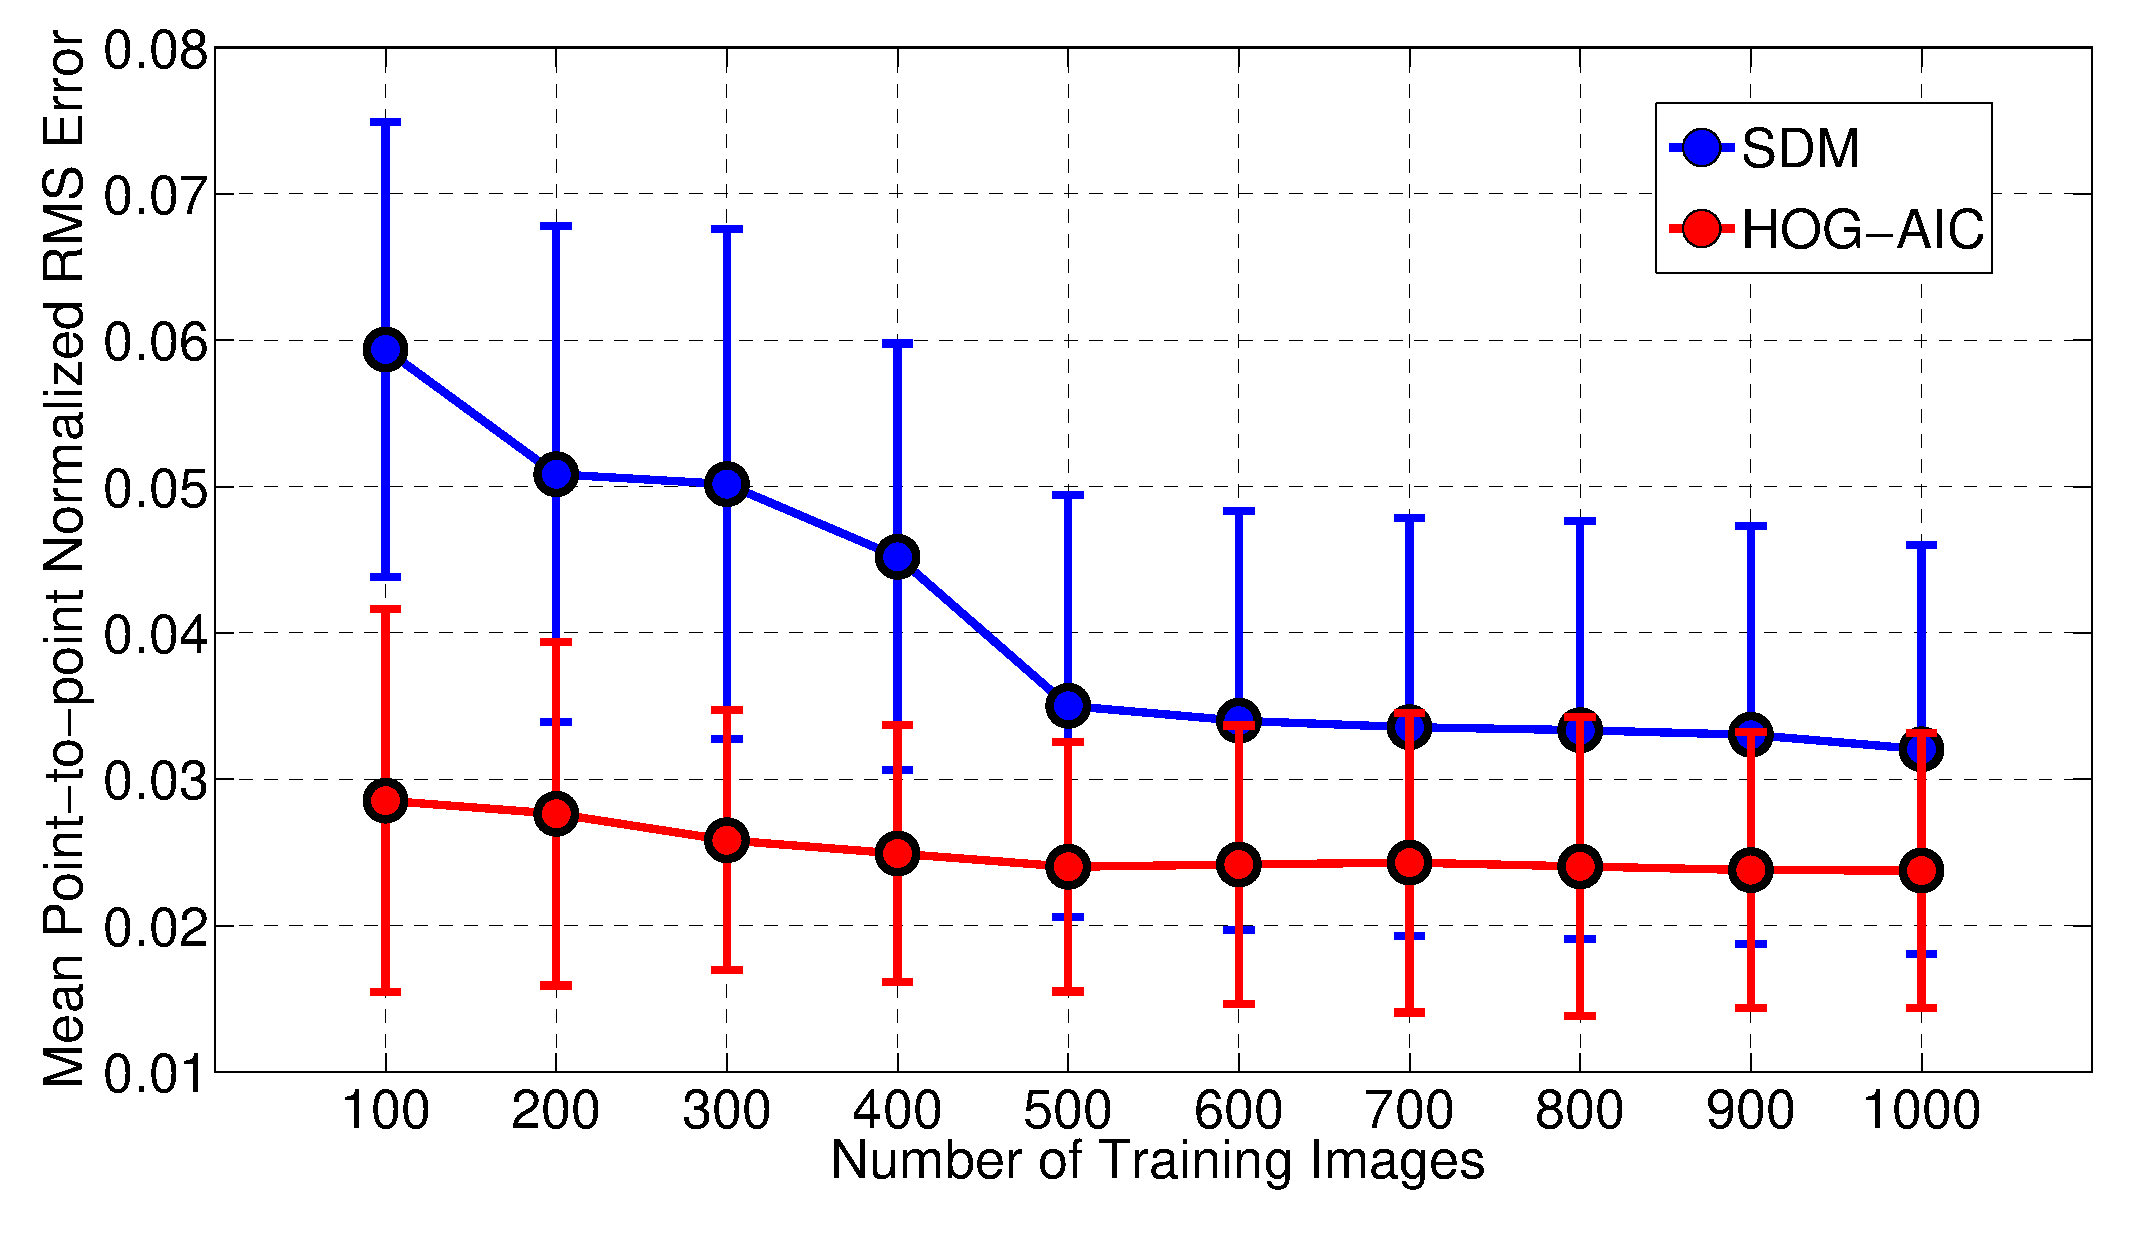
\includegraphics[width=0.70\linewidth]{figures/feature_based_aam/12_NumberOfTrainingImages/experiment}
\caption{Performance (mean and standard deviation) of SIFT-AIC and SDM with
respect to the number of training images. The performance is evaluated on Helen
testset and is measured with the mean and standard deviation of the normalized
RMS error. In this experiment we use our SDM implementation~\cite{menpo2014}.}
\label{fig:numberOfTrainingImages}
\end{figure}
%

% Comparison with state-of-the-art
\begin{figure}[!t]
\centering
\hspace{0.6cm}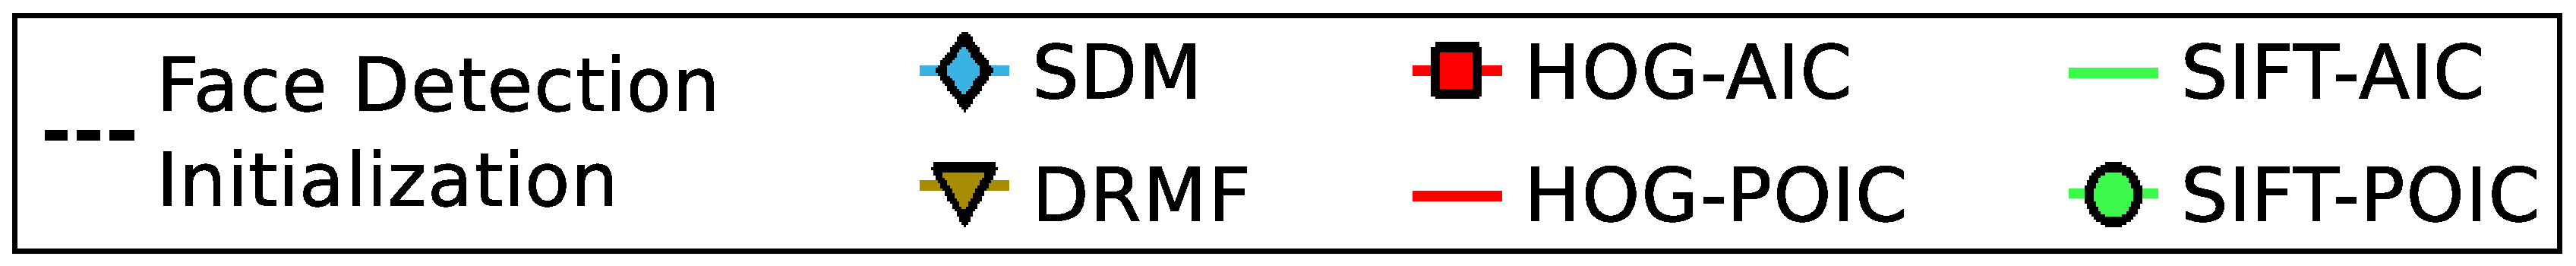
\includegraphics[height=0.85cm]{figures/feature_based_aam/13_AAMcomparison/legend}\\
\includegraphics[width=0.70\linewidth]{figures/feature_based_aam/13_AAMcomparison/LFPWtest}
\caption{Comparison between our proposed HOG and SIFT AAMs and two
state-of-the-art methods (SDM~\cite{xiong2013supervised} and
DRMF~\cite{asthana2013robust}) on LFPW testset. The evaluation is based on 49
points mask, which means it does not include the face boundary (jaw). For SDM
and DRMF we use the code provided by their authors.}
\label{fig:comparison:LFPWtest}
\end{figure}
%
\begin{figure}[!t]
\centering
\hspace{0.6cm}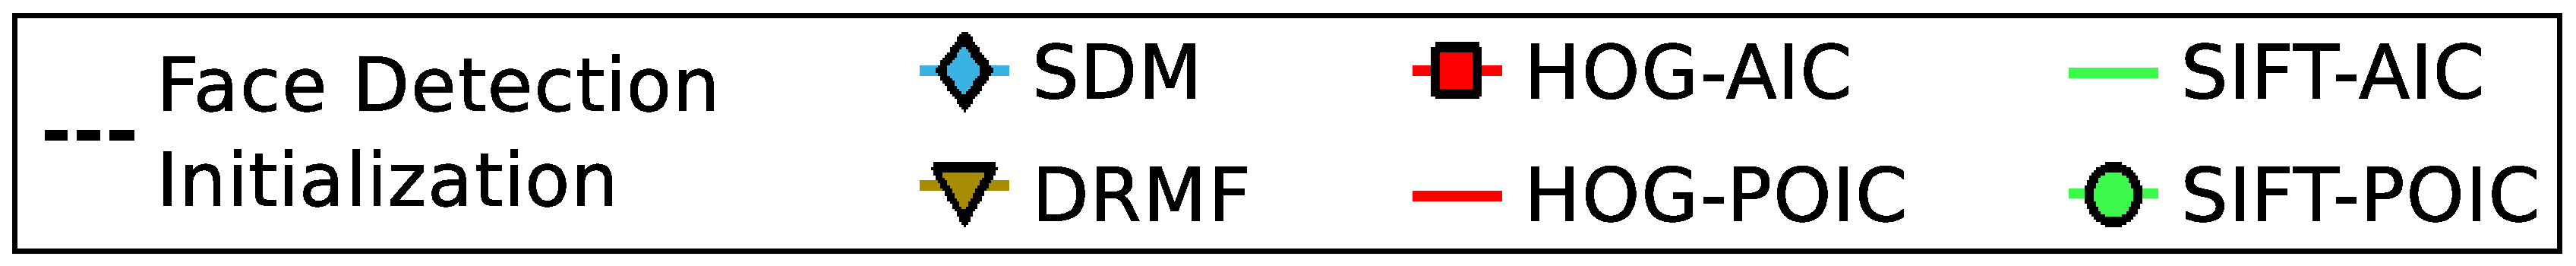
\includegraphics[height=0.85cm]{figures/feature_based_aam/13_AAMcomparison/legend}\\
\includegraphics[width=0.70\linewidth]{figures/feature_based_aam/13_AAMcomparison/Helen}
\caption{Comparison between our proposed HOG and SIFT AAMs and two
state-of-the-art methods (SDM~\cite{xiong2013supervised} and
DRMF~\cite{asthana2013robust}) on Helen trainset and testset. The evaluation is
based on 49 points mask, which means it does not include the face boundary
(jaw). For SDM and DRMF we use the code provided by their authors.}
\label{fig:comparison:Helen}
\end{figure}
%
\begin{figure}[!t]
\centering
\hspace{0.6cm}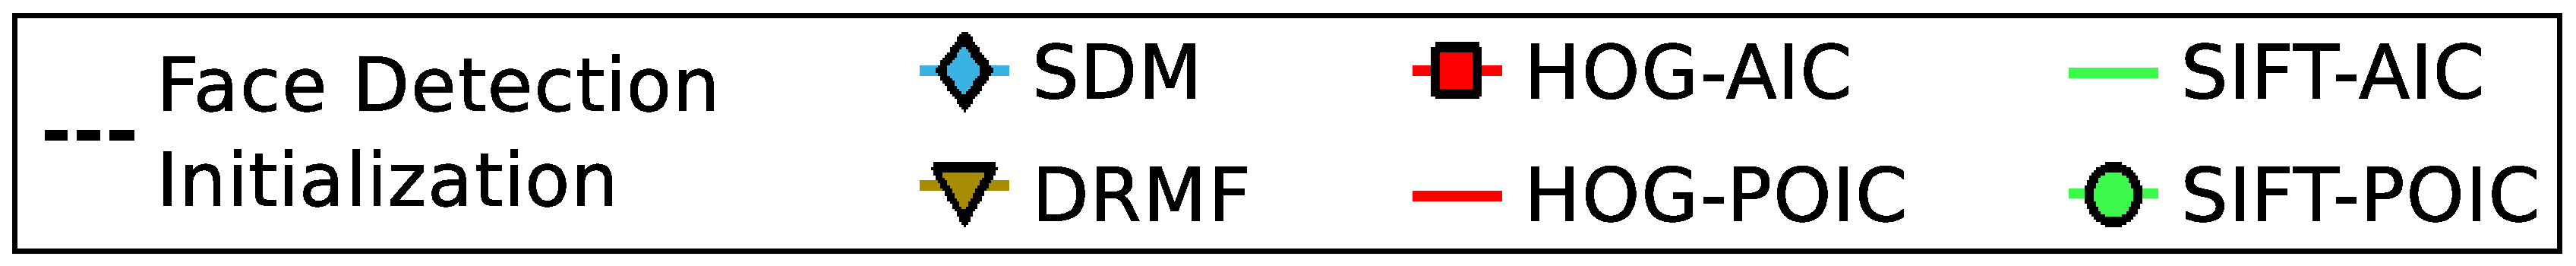
\includegraphics[height=0.85cm]{figures/feature_based_aam/13_AAMcomparison/legend}\\
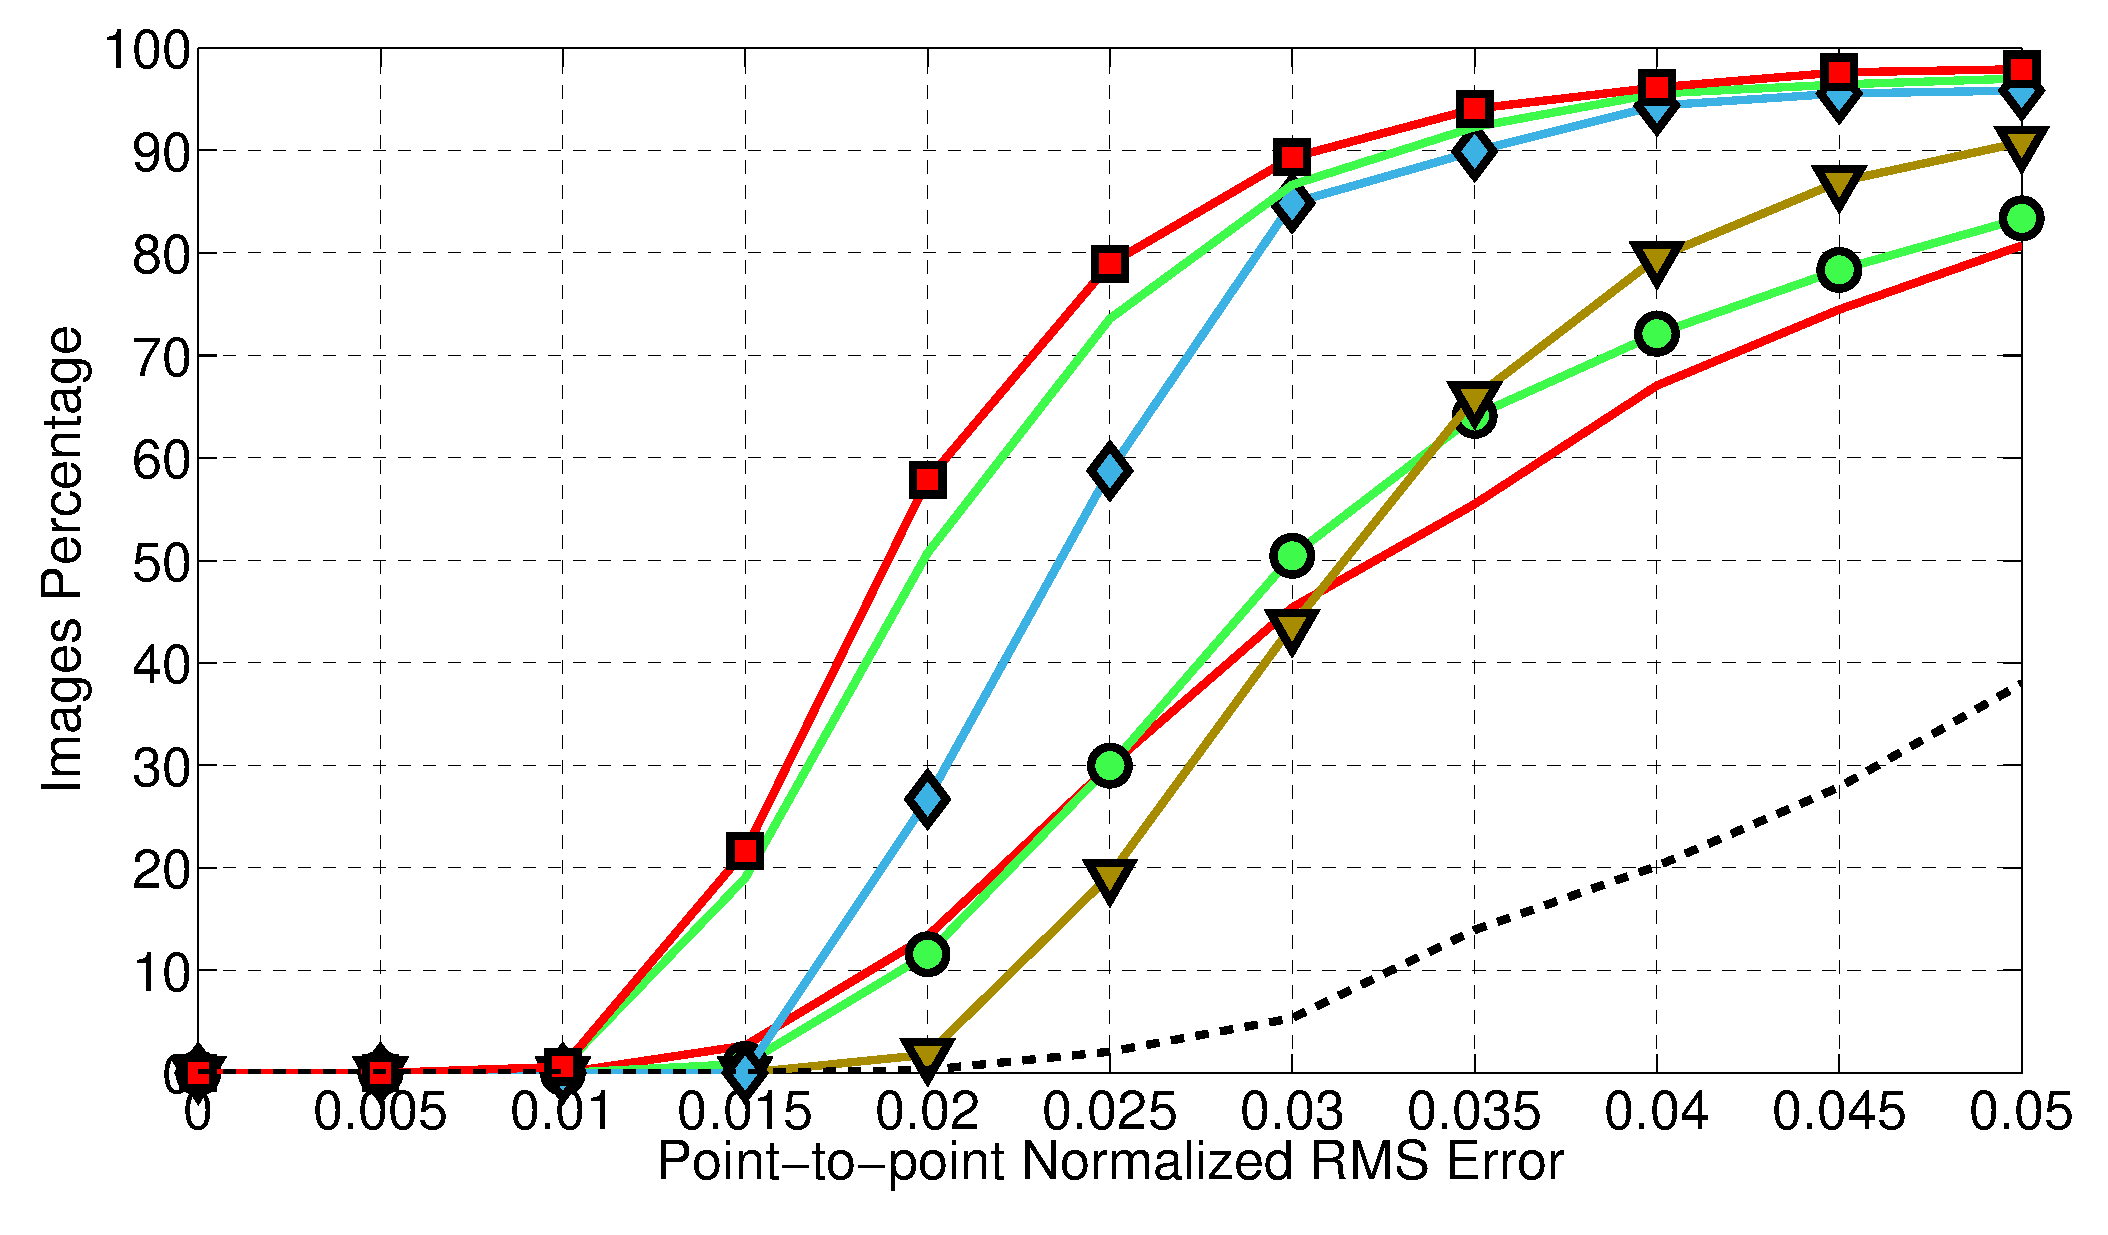
\includegraphics[width=0.70\linewidth]{figures/feature_based_aam/13_AAMcomparison/AFW}
\caption{Comparison between our proposed HOG and SIFT AAMs and two
state-of-the-art methods (SDM~\cite{xiong2013supervised} and
DRMF~\cite{asthana2013robust}) on AFW. The evaluation is based on 49
points mask, which means it does not include the face boundary (jaw). For SDM
and DRMF we use the code provided by their authors.}
\label{fig:comparison:AFW}
\end{figure}
%
\begin{figure}[!t]
\centering
\hspace{0.6cm}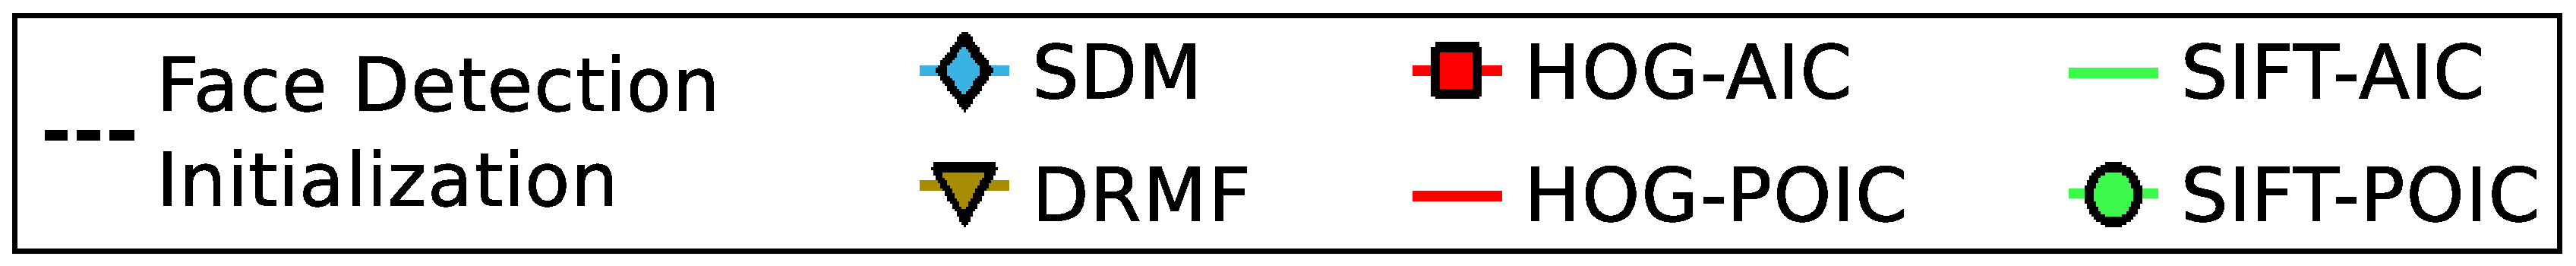
\includegraphics[height=0.85cm]{figures/feature_based_aam/13_AAMcomparison/legend}\\
\includegraphics[width=0.70\linewidth]{figures/feature_based_aam/13_AAMcomparison/iBUG}
\caption{Comparison between our proposed HOG and SIFT AAMs and two
state-of-the-art methods (SDM~\cite{xiong2013supervised} and
DRMF~\cite{asthana2013robust}) on iBUG. The evaluation is based on 49
points mask, which means it does not include the face boundary (jaw). For SDM
and DRMF we use the code provided by their authors.}
\label{fig:comparison:iBUG}
\end{figure}
%

Figures~\ref{fig:comparison:LFPWtest}-\ref{fig:comparison:iBUG} show the
results on LFPW testset, AFW, iBUG and Helen train and test databases,
respectively (3026 images in total). A main difference between
these two methods and AAMs is that due to their discriminative nature, they both
require many data in order to generalize well, whilst the generative shape and
appearance models of AAMs perform well with much fewer training images. This is
shown in Fig.~\ref{fig:numberOfTrainingImages} which plots the performance of
HOG-AIC and SDM with respect to the number of training images. Since SDMs's authors do not provide any training code~\cite{xiong2013supervised}, for this small experiment we employ our SDM version developed in the Menpo Project~\cite{menpo2014}.
The training images are randomly selected from the 2811 images of LFPW and Helen
trainsets and the evaluation is applied on Helen testing set. The graph shows
that SDM keeps improving as the number of training images increases whilst the
SIFT AAMs performance remains almost the same. Finally,
Fig.~\ref{fig:afw-helen-images} shows some indicative fitting results using all
the features employed in this work.

The results indicate that HOG-AIC and SIFT-AIC significantly outperform DRMF and
are also more accurate than SDM. They are more accurate especially when they
converge as can be seen from the percentage of images with error less or equal
than $0.02$. Even though SDM and DRMF have smaller computational complexities
compared to Tab.~\ref{tab:times}, we find these results remarkable, considering
that our feature-based AAMs are trained using much fewer training images.
Finally, the results show that the HOG and SIFT POIC models have a similar
performance as DRMF.

% Fitting examples
\begin{figure}[!t]
\centering
\subfloat[Face Detection Initialization]{
\includegraphics[width=0.104\textwidth]{figures/feature_based_aam/14_FittingImages/HOG/Subject45-1}
\includegraphics[width=0.104\textwidth]{figures/feature_based_aam/14_FittingImages/HOG/Subject21-1}
\includegraphics[width=0.104\textwidth]{figures/feature_based_aam/14_FittingImages/HOG/Subject65-1}
\includegraphics[width=0.104\textwidth]{figures/feature_based_aam/14_FittingImages/HOG/Subject68-1}
\includegraphics[width=0.104\textwidth]{figures/feature_based_aam/14_FittingImages/HOG/Subject56-1}
\includegraphics[width=0.104\textwidth]{figures/feature_based_aam/14_FittingImages/HOG/Subject64-1}
\includegraphics[width=0.104\textwidth]{figures/feature_based_aam/14_FittingImages/HOG/Subject20-1}
\includegraphics[width=0.104\textwidth]{figures/feature_based_aam/14_FittingImages/HOG/Subject26-1}
\includegraphics[width=0.104\textwidth]{figures/feature_based_aam/14_FittingImages/HOG/Subject61-1}}\vspace{-0.2cm}\\
%
\subfloat[HOG]{
\includegraphics[width=0.104\textwidth]{figures/feature_based_aam/14_FittingImages/HOG/Subject45-2}
\includegraphics[width=0.104\textwidth]{figures/feature_based_aam/14_FittingImages/HOG/Subject21-2}
\includegraphics[width=0.104\textwidth]{figures/feature_based_aam/14_FittingImages/HOG/Subject65-2}
\includegraphics[width=0.104\textwidth]{figures/feature_based_aam/14_FittingImages/HOG/Subject68-2}
\includegraphics[width=0.104\textwidth]{figures/feature_based_aam/14_FittingImages/HOG/Subject56-2}
\includegraphics[width=0.104\textwidth]{figures/feature_based_aam/14_FittingImages/HOG/Subject64-2}
\includegraphics[width=0.104\textwidth]{figures/feature_based_aam/14_FittingImages/HOG/Subject20-2}
\includegraphics[width=0.104\textwidth]{figures/feature_based_aam/14_FittingImages/HOG/Subject26-2}
\includegraphics[width=0.104\textwidth]{figures/feature_based_aam/14_FittingImages/HOG/Subject61-2}}\vspace{-0.2cm}\\
%
\subfloat[SIFT]{
\includegraphics[width=0.104\textwidth]{figures/feature_based_aam/14_FittingImages/SIFT/Subject45-2}
\includegraphics[width=0.104\textwidth]{figures/feature_based_aam/14_FittingImages/SIFT/Subject21-2}
\includegraphics[width=0.104\textwidth]{figures/feature_based_aam/14_FittingImages/SIFT/Subject65-2}
\includegraphics[width=0.104\textwidth]{figures/feature_based_aam/14_FittingImages/SIFT/Subject68-2}
\includegraphics[width=0.104\textwidth]{figures/feature_based_aam/14_FittingImages/SIFT/Subject56-2}
\includegraphics[width=0.104\textwidth]{figures/feature_based_aam/14_FittingImages/SIFT/Subject64-2}
\includegraphics[width=0.104\textwidth]{figures/feature_based_aam/14_FittingImages/SIFT/Subject20-2}
\includegraphics[width=0.104\textwidth]{figures/feature_based_aam/14_FittingImages/SIFT/Subject26-2}
\includegraphics[width=0.104\textwidth]{figures/feature_based_aam/14_FittingImages/SIFT/Subject61-2}}\vspace{-0.2cm}\\
%
\subfloat[IGO]{
\includegraphics[width=0.104\textwidth]{figures/feature_based_aam/14_FittingImages/IGO/Subject45-2}
\includegraphics[width=0.104\textwidth]{figures/feature_based_aam/14_FittingImages/IGO/Subject21-2}
\includegraphics[width=0.104\textwidth]{figures/feature_based_aam/14_FittingImages/IGO/Subject65-2}
\includegraphics[width=0.104\textwidth]{figures/feature_based_aam/14_FittingImages/IGO/Subject68-2}
\includegraphics[width=0.104\textwidth]{figures/feature_based_aam/14_FittingImages/IGO/Subject56-2}
\includegraphics[width=0.104\textwidth]{figures/feature_based_aam/14_FittingImages/IGO/Subject64-2}
\includegraphics[width=0.104\textwidth]{figures/feature_based_aam/14_FittingImages/IGO/Subject20-2}
\includegraphics[width=0.104\textwidth]{figures/feature_based_aam/14_FittingImages/IGO/Subject26-2}
\includegraphics[width=0.104\textwidth]{figures/feature_based_aam/14_FittingImages/IGO/Subject61-2}}\vspace{-0.2cm}\\
%
\subfloat[ES]{
\includegraphics[width=0.104\textwidth]{figures/feature_based_aam/14_FittingImages/ES/Subject45-2}
\includegraphics[width=0.104\textwidth]{figures/feature_based_aam/14_FittingImages/ES/Subject21-2}
\includegraphics[width=0.104\textwidth]{figures/feature_based_aam/14_FittingImages/ES/Subject65-2}
\includegraphics[width=0.104\textwidth]{figures/feature_based_aam/14_FittingImages/ES/Subject68-2}
\includegraphics[width=0.104\textwidth]{figures/feature_based_aam/14_FittingImages/ES/Subject56-2}
\includegraphics[width=0.104\textwidth]{figures/feature_based_aam/14_FittingImages/ES/Subject64-2}
\includegraphics[width=0.104\textwidth]{figures/feature_based_aam/14_FittingImages/ES/Subject20-2}
\includegraphics[width=0.104\textwidth]{figures/feature_based_aam/14_FittingImages/ES/Subject26-2}
\includegraphics[width=0.104\textwidth]{figures/feature_based_aam/14_FittingImages/ES/Subject61-2}}\vspace{-0.2cm}\\
%
\subfloat[Gabor Angles]{
\includegraphics[width=0.104\textwidth]{figures/feature_based_aam/14_FittingImages/GaborAngles/Subject45-2}
\includegraphics[width=0.104\textwidth]{figures/feature_based_aam/14_FittingImages/GaborAngles/Subject21-2}
\includegraphics[width=0.104\textwidth]{figures/feature_based_aam/14_FittingImages/GaborAngles/Subject65-2}
\includegraphics[width=0.104\textwidth]{figures/feature_based_aam/14_FittingImages/GaborAngles/Subject68-2}
\includegraphics[width=0.104\textwidth]{figures/feature_based_aam/14_FittingImages/GaborAngles/Subject56-2}
\includegraphics[width=0.104\textwidth]{figures/feature_based_aam/14_FittingImages/GaborAngles/Subject64-2}
\includegraphics[width=0.104\textwidth]{figures/feature_based_aam/14_FittingImages/GaborAngles/Subject20-2}
\includegraphics[width=0.104\textwidth]{figures/feature_based_aam/14_FittingImages/GaborAngles/Subject26-2}
\includegraphics[width=0.104\textwidth]{figures/feature_based_aam/14_FittingImages/GaborAngles/Subject61-2}}\vspace{-0.2cm}\\
%
\subfloat[Gabor Magnitude]{
\includegraphics[width=0.104\textwidth]{figures/feature_based_aam/14_FittingImages/GaborMagnitude/Subject45-2}
\includegraphics[width=0.104\textwidth]{figures/feature_based_aam/14_FittingImages/GaborMagnitude/Subject21-2}
\includegraphics[width=0.104\textwidth]{figures/feature_based_aam/14_FittingImages/GaborMagnitude/Subject65-2}
\includegraphics[width=0.104\textwidth]{figures/feature_based_aam/14_FittingImages/GaborMagnitude/Subject68-2}
\includegraphics[width=0.104\textwidth]{figures/feature_based_aam/14_FittingImages/GaborMagnitude/Subject56-2}
\includegraphics[width=0.104\textwidth]{figures/feature_based_aam/14_FittingImages/GaborMagnitude/Subject64-2}
\includegraphics[width=0.104\textwidth]{figures/feature_based_aam/14_FittingImages/GaborMagnitude/Subject20-2}
\includegraphics[width=0.104\textwidth]{figures/feature_based_aam/14_FittingImages/GaborMagnitude/Subject26-2}
\includegraphics[width=0.104\textwidth]{figures/feature_based_aam/14_FittingImages/GaborMagnitude/Subject61-2}}\vspace{-0.2cm}\\
%
\subfloat[OLBP]{
\includegraphics[width=0.104\textwidth]{figures/feature_based_aam/14_FittingImages/OLBP/Subject45-2}
\includegraphics[width=0.104\textwidth]{figures/feature_based_aam/14_FittingImages/OLBP/Subject21-2}
\includegraphics[width=0.104\textwidth]{figures/feature_based_aam/14_FittingImages/OLBP/Subject65-2}
\includegraphics[width=0.104\textwidth]{figures/feature_based_aam/14_FittingImages/OLBP/Subject68-2}
\includegraphics[width=0.104\textwidth]{figures/feature_based_aam/14_FittingImages/OLBP/Subject56-2}
\includegraphics[width=0.104\textwidth]{figures/feature_based_aam/14_FittingImages/OLBP/Subject64-2}
\includegraphics[width=0.104\textwidth]{figures/feature_based_aam/14_FittingImages/OLBP/Subject20-2}
\includegraphics[width=0.104\textwidth]{figures/feature_based_aam/14_FittingImages/OLBP/Subject26-2}
\includegraphics[width=0.104\textwidth]{figures/feature_based_aam/14_FittingImages/OLBP/Subject61-2}}\vspace{-0.2cm}\\
%
\subfloat[TPLBP (similar for FPLBP)]{
\includegraphics[width=0.104\textwidth]{figures/feature_based_aam/14_FittingImages/TPLBP/Subject45-2}
\includegraphics[width=0.104\textwidth]{figures/feature_based_aam/14_FittingImages/TPLBP/Subject21-2}
\includegraphics[width=0.104\textwidth]{figures/feature_based_aam/14_FittingImages/TPLBP/Subject65-2}
\includegraphics[width=0.104\textwidth]{figures/feature_based_aam/14_FittingImages/TPLBP/Subject68-2}
\includegraphics[width=0.104\textwidth]{figures/feature_based_aam/14_FittingImages/TPLBP/Subject56-2}
\includegraphics[width=0.104\textwidth]{figures/feature_based_aam/14_FittingImages/TPLBP/Subject64-2}
\includegraphics[width=0.104\textwidth]{figures/feature_based_aam/14_FittingImages/TPLBP/Subject20-2}
\includegraphics[width=0.104\textwidth]{figures/feature_based_aam/14_FittingImages/TPLBP/Subject26-2}
\includegraphics[width=0.104\textwidth]{figures/feature_based_aam/14_FittingImages/TPLBP/Subject61-2}}\vspace{-0.2cm}\\
%
\subfloat[Intensities]{
\includegraphics[width=0.104\textwidth]{figures/feature_based_aam/14_FittingImages/Intensities/Subject45-2}
\includegraphics[width=0.104\textwidth]{figures/feature_based_aam/14_FittingImages/Intensities/Subject21-2}
\includegraphics[width=0.104\textwidth]{figures/feature_based_aam/14_FittingImages/Intensities/Subject65-2}
\includegraphics[width=0.104\textwidth]{figures/feature_based_aam/14_FittingImages/Intensities/Subject68-2}
\includegraphics[width=0.104\textwidth]{figures/feature_based_aam/14_FittingImages/Intensities/Subject56-2}
\includegraphics[width=0.104\textwidth]{figures/feature_based_aam/14_FittingImages/Intensities/Subject64-2}
\includegraphics[width=0.104\textwidth]{figures/feature_based_aam/14_FittingImages/Intensities/Subject20-2}
\includegraphics[width=0.104\textwidth]{figures/feature_based_aam/14_FittingImages/Intensities/Subject26-2}
\includegraphics[width=0.104\textwidth]{figures/feature_based_aam/14_FittingImages/Intensities/Subject61-2}}
%
\caption{Fitting examples using feature-based AIC on very challenging images from iBUG database.}
\label{fig:afw-helen-images}
\end{figure}
%

% Results Interpretation and Discussion
\subsection{Results Interpretation and Discussion}\label{subsec:aam:discussion}
In general, it is very difficult to find a strict theoretical difference between
the various employed non-linear features, such as HOG, SIFT, LBP etc., because
the design of features still remains mainly an empirical art rather than an exact
science. Nevertheless, we can sketch the difference between the magnitude of Gabor
filters in various scales and orientations and SIFT features. Gabor features have
been used before in literature~\cite{lucey2013fourier,gao2009gabor}, however
our experiments prove that they are not efficient for generic face alignment and
are probably more suitable for person-specific settings~\cite{wiskott1997face,duc1999face}.

The difference between the complex response (i.e., having both the magnitude and
the phase) of Gabor filters and other employed features is that the former are
produced by the convolution of a bank of linear filters, hence they are not robust
to the facial appearance changes~\cite{lucey2013fourier}. This is the reason why
we prefer to extract non-linear features from the responses, i.e. the magnitude
(modulus) and the phase. Moreover, the difference between the magnitude of Gabor
filters in various scales and orientations and SIFT features can be explained
using the theory on invariant scattering networks~\cite{bruna2013invariant},
according to which SIFT features can be very well approximated by the modulus of
the coefficients of the wavelet transform using a particular family of wavelets
(i.e. partial derivatives of a Gaussian) (for more details please refer to
Section 2.3 of~\cite{bruna2013invariant}). Convolution with Gabor filters with
different scales and orientations does not constitute a proper wavelet image
transform. In general Gabor filter expansion is not applied in building a wavelet
transform, since this requires computation of bi-orthogonal wavelets, which may
be very time-consuming. Therefore, usually a filter bank consisting of Gabor
filters with various scales and rotations~\cite{wiskott1997face,duc1999face},
as we do in this work, is created and applied for feature extraction. In general,
the results suggest that large-scale features are very robust and have a high
convergence frequency even with initializations that are too far from ground-truth.
However, when the initialization is close to the optimal solution, higher-frequency
features tend to be more accurate. For example the phase filter information may
have excellent localization properties when the deformation is small, but it is
very sensitive to noise and small perturbations.

Finally, we believe that the advantages of the employed features, especially
the multi-channel gradient based ones such as HOG and SIFT, are excellently
coupled with the generalization ability of generative models. In fact, we believe
that the most important experimental result shown in the previous section is
that the combination of
\begin{enumerate}
  \item non-linear least-squares optimization, with
  \item robust features, and
  \item generative models
\end{enumerate}
can achieve very good performance without the need of large training datasets,
which emphasizes the main advantage of the proposed framework over
discriminative methods.
